\documentclass[11pt,a4paper]{report}
\usepackage{listings,textcomp,graphicx,float,verbatim,extsizes}
\usepackage{amsmath,amssymb,mathrsfs}
\usepackage{here}
\usepackage{subfig}
\usepackage{multicol}
\usepackage{sectsty}
\usepackage{algorithm}
\usepackage{algpseudocode}

\usepackage[left=3.2cm, right=3.2cm, top=3cm, bottom=4cm]{geometry}

%setup links
\usepackage{hyperref}
\hypersetup{
    colorlinks,
    citecolor=black,
    filecolor=black,
    linkcolor=black,
    urlcolor=black
}
%\hypersetup{linktocpage} to only make page number in toc clickable

\usepackage{fancyhdr}

\pagestyle{fancy}
\setlength{\headheight}{15.2pt}
\fancyhead[LE,RO]{\slshape \rightmark}
\fancyhead[LO,RE]{\slshape \leftmark}
\fancyfoot[C]{\thepage}
\begin{comment}

\lhead{}
\chead{}
\rhead{}
\lfoot{}
\cfoot{\thepage}
\rfoot{}


\makeatletter
\renewcommand{\@makechapterhead}[1]{%
\vspace*{50 pt}%
{\setlength{\parindent}{0pt} \raggedright \normalfont
\bfseries\Huge
\ifnum \value{secnumdepth}>1
   \if@mainmatter\thechapter.\ \fi%
\fi
#1\par\nobreak\vspace{40 pt}}}
\makeatother
\end{comment}
\begin{document}

\setcounter{secnumdepth}{3}
\setcounter{tocdepth}{3}

%pmatrix with vertical bar
\makeatletter
\renewcommand*\env@matrix[1][*\c@MaxMatrixCols c]{%
  \hskip -\arraycolsep
  \let\@ifnextchar\new@ifnextchar
  \array{#1}}
\makeatother

\begin{titlepage}

\begin{center}


\textsc{\LARGE Imperial College London}\\[3.5cm]


{ \huge \bfseries Expression Transfer}\\[5.5cm]



% Author and supervisor
\begin{minipage}{0.4\textwidth}
\begin{flushleft} \large
\emph{Author:}\\
Martin \textsc{Papanek}
\end{flushleft}
\end{minipage}
\begin{minipage}{0.4\textwidth}
\begin{flushright} \large
\emph{Supervisor:} \\
Professor ~Duncan \textsc{Gillies}
\end{flushright}
\end{minipage}

\vfill

% Bottom of the page
{\large \today}

\end{center}

\end{titlepage}

\begin{center}
\LARGE \textbf{Abstract}
\end{center}

\newpage

\begin{center}
\LARGE \textbf{Acknowledgments}
\end{center}



\tableofcontents

\chapter{Introduction}
\section{Motivation}
Allowing computers to understand the world around them is one of the most
intriguing goals of computer science. In order to aid humans in day-to-day
tasks, the ideal computer should be able to perceive its surroundings, correctly identify the objects and beings around it and act based
on this information. Achieving this level of sophisticated, environment-aware
behavior is the focus of popular computer science fields such as machine
learning, computer vision and logic.

The problem of understanding the surrounding world can be broken down into a
number of sub-problems. First the machine must obtain and process the information on
its sensors. Then it has to process this data in order to find objects in the
sensory input. Finally, the machine has to assign meaning to the scene it perceived
based on the the configuration and the properties of the objects it found. This
allows the machine to understand what state the environment is in and it may
then utilize this information using simple if-then rules.

For humans, all of the aforementioned sub-problems seem simple. However, programming
machines to perform these tasks has proven to be quite difficult. Computers often do
possess better sensors than most humans and thus are readily able to obtain data
from sensors. Yet, they are sorely lacking when it comes to locating objects
in this sensory input and correctly assessing the properties and configuration
of these objects. While it is possible to locate circles and lines, joining
these to locate a face or a tree can only be done if the machine knows what a
face or a tree should look like. Thus, the machine needs to have prior
information about the objects it can expect. This prior information can be
encoded in a \textit{model}. The model describes the structure of the object.
This, in turn, allows the machine to explain aspects of its sensory input as the
an instance of this model.

Certain objects may also change their shape or
appearance. For example a face may transition from a closed eyed state to an
open eyed state. An even better example is the body of a human, which is also
highly dynamic. These deformable objects are often of special interest to us in
our everyday life. A machine should therefore be able to recognize an arbitrarily deformed
object and also correctly identify the the degree of deformation, since the amount of deformation may be crucial for the understanding of
the scene. The challenge thus lies in constructing an appropriate \textit{deformable
model}. 

Given a deformable model, the machine then has to process the sensor input and
locate instances of the model by adjusting the model parameters. This task is
known as \textit{model-based recognition}. The parameters of the model allow the
machine to interpret the scene. 

In addition to locating an instance of the model
in a single sensory input the machine should also be able to track movement of
this instance given a sequence of snapshots of
the environment. The task of identifying and tracking an instance of a model from
one sensory snapshot to another, in spite of deformations of shape
and changes in position, is known as \textit{model-based tracking}.

This paper will describe convenient deformable shape
and appearance models and effective algorithms for locating these
models. Sensory snapshots will be limited exclusively to images of the environment. As we will be dealing
with images we will investigate motion tracking algorithms. These are necessary
to follow optical cues in our input image which makes it possible to track the
movements of the model through successive images.

\section{Contributions}

The area where deformable models are applicable is quite large. We will focus on one very interesting application of dynamical
models and model extraction which is
\textit{expression transfer}. The purpose of expression transfer is to capture
the expressions from a video recording of one individual and
generate a video of another individual mimicking these
expressions. The alternative to transferring these expressions would
be to construct a physical model of the face and simulate the observed
expressions from scratch by manipulating the parameters of the model. The
advantage of transferring the dynamics of a subjects face to that of another is
that it enables us to
create very realistic animations without too much user intervention. 

The paper describes the developement of an expression transfer application, which combines motion tracking and a deformable
model to gain understanding of the face deformations present an the input video
recording. 

We make the following contributions
\begin{itemize}
\item Developed an expression transfer application complete with a graphical
  user interface. 
\item Formalized an algorithm for expression transfer using a deformable model
  of face shapes (Section \ref{s:exptranalgo}).
\item Derived a fitting algorithm for finding the deformable model
  parameters from an image (Sections \ref{s:minerror} and \ref{s:fitalgo}).
\item Elucidated a multilinear deformable model desgined for expression
  transfer (Section \ref{s:hosvd}). 
\end{itemize}

\newpage

\chapter{Background}
Considerable amount of research has been done on using models to characterize a
deformable object as well as on model-based object recognition and
tracking. In this chapter we will present an overview of various modeling techniques. Likewise, we will discuss
computer vision algorithms which will allow us to locate and track features of
interest in the image. These features are necessary to fit an instance
of the model to the image.

\section{Deformable Models}
Models give the computer prior information about the structure of a class of objects. Most
real world objects have a dynamic structure. To allow the computer to locate
such dynamic objects it is necessary to account for this variability by giving the
computer prior information about the possible variations. A deformable model
describes the expected structure of a class of objects while at the same time allowing
for variations from the expected structure. Thus, if a somewhat deformed
instance of this class of objects is present in the image, the deformable model
will be able to explain this is as a deformation from the expected shape.

The quality of a deformable model can be assessed based on two important
characteristics. First, the model should be \textit{general} enough so that it
is capable of representing any realistic deformation of the object.
On the other hand, the computer should only to be able to find an instance of this
model in its surroundings if and only if this object is present. The deformable model
therefore has to be \textit{specific} so that it does not locate non-existent
instances of a model in the input. Clearly, a model that is too general will inadvertently fit objects from a
different class and, vice versa, a model that is too specific will not be able to
explain all the variations of the object structure and will thus fail to locate
instances of the correct class. The optimal deformable model must balance
generality and specificity.

The variance in shape or appearance of a model may be due to combination of the following
factors:
\begin{itemize}
\item Variations of shape due to deformations of the object.
\item Arbitrary scaling of the object, possibly due to distance from the observer.
\item Arbitrary rotations of the object which may cause occlusions. 
\item Some measure of Gaussian input noise.
\item Differences in color or intensity caused by a change in lighting conditions.
\end{itemize}
Some of these sources of variation may be explained away using standard machine
vision techniques. Noisy input can be explained by means of Gaussian
filtering. However, other sources of variation such as those due to deformations of the
object need to be represented by appropriate parameters of the model. This is
where a deformable model becomes necessary. The
deformable model simulates deformations based on the parameter values. Thus, to
construct the model, the mapping from parameters to deformations must be learned. The two
most prevalent approaches to discovering this mapping are using either \textit{physical
models} or \textit{statistical models}.

Physical models construct deformable models which mimic the elastic deformations
of the class of object they model. The parameters of a physical model control the amount
of actual physical deformation.

Statistical deformable models are trained on a set of examples of a class of
objects. With this group of models, a basis for the deformations observed in
this set of examples is constructed through statistical analysis. This basis then allows the model to predict
probable instances of the objects of this class. 

An important subgroup of statistical models are the \textit{tensor models}. The
tensor models are obtained using a mathematical generalization of statistical analysis
techniques in higher dimensions.

Finally, given that a deformable model is uniquely defined by its parameters,
 the goal of model-based object recognition is then to fit an instance of a model to
an appropriate object in the image. The problem of fitting the model to the
image is essentially an optimization problem. In order to fit the model we need to
correctly adjust parameters that control the model. In addition to determining
the intrinsic parameters of the model it is necessary to also find how the
object is rotated, moved and scaled to explain the variation in structure which
is not caused by the deformations. The recognition algorithm also needs to be
robust enought to be able to deal with variations caused by noise.

\subsection{Physics Based Models}
Natural objects all obey physical laws. Human and animal bodies change shape
when their muscles contract and loosen, which in turn alters the shape of the
elastic soft tissues which surround the muscles. Movement is further constrained
by the skeleton and gravity. Due to the dynamic nature of such objects it is quite impractical to
model the structure of these objects as consisting of only rigid components. To cope with
such highly dynamic bodies researchers have turned to physics to describe the
rules governing these dynamics in form of a set of equations. Pentland and
Sclaroff in  \cite{FEM1pen} give a closed form solution for extracting a
physical model from images. Terzopoulos and Metaxas combine physics-based
deformable models with Kalman filtering theory in \cite{FEM1ter}.  

As the name suggests, physical models emulate the physical laws that govern
deformations. Physical models are predominantly formulated using the finite
element analysis. An in depth discussion of finite element
analysis can be found in \cite{FEMbook}.

\subsubsection{Finite Element Method (FEM)}
The FEM method is a numerical engineering technique for the simulation of dynamic
behavior of solids and structures. With the finite element method the assumption is made that
the object alters shape as if it were made of a clay-like material. In physics,
\textit{strain} is the measure of deformation or displacement from a rigid body state. The stiffness
of the material determines responses to strain and stress and thus describes the
degrees of freedom of the material.

The underlying idea behind FEM is that the object is approximated as an
assemblage of elements of finite size. These elements are interconnected with
each other by nodal points throughout the object. The structure of an object is
thus discretized into a mesh of $N$ finite elements. The elements are placed
next to each other so that no gaps remain in between. When the object undergoes a
deformation, this in turn propagates through the mesh of finite elements which
themselves deform accordingly. The displacements within these elements are assumed to be a function
of the displacements measured at the nodal points. This assumption is
fundamental for the FEM and can be formalized as
\begin{equation}\label{eq:FEMdisplacements}
u^{(m)}(x,y,z) = \mathbf{H}^{(m)}(x,y,z)*\mathbf{U}
\end{equation}
where $u^{(m)}$ is the displacement at $x$, $y$, and $z$ coordinate within the element $m$, $\mathbf{H}^{(m)}$
the displacement interpolation matrix and $\mathbf{U}$ the global
displacement measured at every nodal point. With equation
\ref{eq:FEMdisplacements} the displacements at any point in the object can be calculated.
The values of the displacement interpolation matrix $\mathbf{H}^{(m)}$ depend on
the shape of the finite elements that make up the mesh.

From the displacement $u^{(m)}(x,y,z)$, the strain can be calculated as the
derivative of the displacement with respect to $x$, $y$, and $z$. Thus, the
strain $\epsilon^{(m)}(x,y,z)$ at the element $m$ is given by  
\begin{equation}\label{eq:FEMstrain}
\epsilon^{(m)}(x,y,z) = \mathbf{B}^{(m)}(x,y,z)*\mathbf{U}
\end{equation}
where $\mathbf{B}^{(m)}(x,y,z)$ is the strain-displacement matrix. This matrix can
be calculated by differentiating the displacement interpolation matrix
$\mathbf{H}^{(m)}$. With equations \ref{eq:FEMdisplacements} and \ref{eq:FEMstrain} the behavior of
the object structure given a global nodal point displacement $\mathbf{U}$ is
defined. 

The goal of displacement-based finite element analysis is to calculate
unknown nodal point displacements from a known force or load acting on the
object. When a load is applied to the structure of the object it will cause a
deformation of the mesh. The nodal points in the mesh will bounce and move
until they reach a state of equilibrium. It is important to stress that in this equilibrium the shape of the
object is still deformed due the applied force. However, the nodal points may have
assumed new stable positions and hence we refer to it as an equilibrium. The
equation governing the equilibrium is derived using equations
\ref{eq:FEMdisplacements}, \ref{eq:FEMstrain} and the Principle of Virtual
Work \cite{FEMbook}. It relates the stiffness matrix $\mathbf{K}$ and the unknown nodal
displacements $\mathbf{U}$ to the loads $\mathbf{R}$ as follows
\begin{equation}\label{eq:FEMequilibrium}
\mathbf{K}\mathbf{U} = \mathbf{R}
\end{equation}
The stiffness matrix $\mathbf{K}$ is calculated as the sum of the stiffness
matrices $\mathbf{K}^{(m)}$ of the individual finite elements. The
$\mathbf{K}^{(m)}$ are
computed from the strain-displacement matrices $\mathbf{B}^{(m)}$ and the
elasticity matrix $\mathbf{E}^{(m)}$ as
\begin{equation}\label{eq:FEMstiffness}
\mathbf{K} = \sum_m \mathbf{K}^{(m)} = \sum_m \int_{V^{(m)}} \mathbf{B}^{(m)T}
  \mathbf{E}^{(m)} \mathbf{B}^{(m)} dV^{(m)}
\end{equation}
where the integral goes over the volume $V^{(m)}$ of the element $m$. This
approach to computing the stiffness matrix is known as the \textit{direct
  stiffness method}. The displacement interpolation matrix and strain-displacement
interpolation matrix are constructed for each finite element. Their calculation
depends on the displacement interpolation function seen in equation
\ref{eq:FEMdisplacements}. Fortunately, these functions have a well defined
formulation which depends on the degrees of freedom (nodal point connections) of
the element. This formulation, along with numerical integration techniques for
calculating the stiffness matrix can be found in chapter 5 of \cite{FEMbook}. The elasticity matrix relates stress and
strain in the material. Its form depends on the dimensionality of the
element. In a one dimensional element the elasticity matrix is a scalar known as
\textit{Young's Modulus}. The value of Young's Modulus describes the elastic
properties of materials and is computed as the constant ratio between stress and strain
in the material.

Equation \ref{eq:FEMequilibrium} describes a static equilibrium at a specific
point in time. If the loads are applied rapidly then inertial and
energy damping forces must be taken into account. Equation \ref{eq:FEMdynamic} gives
the dynamic form of the FEM equilibrium equation where $\dot{\mathbf{U}}$, $\ddot{\mathbf{U}}$ are the
first and second time derivative of $\mathbf{U}$ respectively.
\begin{equation}\label{eq:FEMdynamic}
\mathbf{M}\ddot{\mathbf{U}} + \mathbf{C}\dot{\mathbf{U}} + \mathbf{K}\mathbf{U}
= \mathbf{R}
\end{equation}
Here $\mathbf{M}$ is the mass matrix and $\mathbf{C}$ the damping matrix. This differential
equation is often referred to as the FEM governing equation. To solve for the
unknown nodal displacements $\mathbf{U}$, standard numerical techniques for solving
differential equations can be used.

\subsubsection{Modal Analysis}
Solving the dynamic equilibrium equation \ref{eq:FEMdynamic} by direct integration
is very costly as shown in \cite{FEMbook}. However, it is possible to diagonalize the system
of equations by changing the finite element displacement basis to a generalized displacement
basis $\Phi$ as 
\begin{equation}
\mathbf{U} = \Phi \mathbf{\tilde{U}}
\end{equation}
The advantage of the new generalized basis can be seen when equation \ref{eq:FEMdynamic} is pre-multiplied from the left by $\Phi^T$
to give
\begin{equation}\label{eq:FEMmodal}
\Phi^T\mathbf{M}\Phi\mathbf{\ddot{\tilde{U}}} + \Phi^T\mathbf{C}\Phi\mathbf{\dot{\tilde{U}}} + \Phi^T\mathbf{K}\Phi^T\mathbf{\tilde{U}}
= \Phi^T\mathbf{R}
\end{equation}
The above equation can be diagonalized if $\Phi$ is chosen as consisting of the $n$ eigenvectors of the eigensolutions $(\omega_1^2,\phi_1)\,,\, \dots \,,(\omega_n^2,\phi_n)$ which solve the eigenproblem
\begin{equation}\label{eq:FEMbasis}
\mathbf{K}\Phi = \Omega^2\mathbf{M}\Phi
\end{equation}
so that 
\begin{align}
\Phi^T\mathbf{K}\Phi &= \Omega^2\\
\Phi^T\mathbf{M}\Phi &= \mathbf{I}
\end{align}
These eigenvectors are the free vibrational modes of the equilibrium equation. Choosing $\Phi$ in this manner transforms equation \ref{eq:FEMmodal} into
\begin{equation}\label{eq:FEMdiag}
\mathbf{\ddot{\tilde{U}}} + \mathbf{\tilde{C}}\mathbf{\dot{\tilde{U}}} + \Omega^2\mathbf{\tilde{U}}
= \mathbf{\tilde{R}}
\end{equation}
Under the assumption that the transformed damping matrix $\mathbf{\tilde{C}}$ is also
diagonal, above equation \ref{eq:FEMdiag} is diagonalized form of equation
\ref{eq:FEMdynamic} since
$\Omega^2$ is a diagonal matrix.
Diagonalizing
decouples the individual components of $\mathbf{U}$. This means that we obtain a
separate differential equation for each component of $\mathbf{U}$ and as such it
is not necessary to compute the inverse of the $\mathbf{K}$. Computing this
inverse is costly and may not always be possible if $\mathbf{U}$ is singular. Thus, the
diagonalized equation \ref{eq:FEMdiag} can be solved for the displacements
$\mathbf{\tilde{U}}$ either in closed form or integrated numerically in fewer steps.

\subsubsection{Recovering shape with FEM} 
Through Modal analysis it is possible to easily generate displacements of an
arbitrary object given its
stiffness matrix $\mathbf{K}$. These displacements deform the object. Since the
matrix $\Phi$ encodes the free vibration modes, it is possible to generate a new
face by taking a vector of weights $\mathbf{u}$ and calculating a deformed
instance of the object class by adding the displacements to the mean shape
$\mathbf{\bar{x}}$ using
\begin{equation}\label{eq:FEMgenerate}
\mathbf{x} =  \mathbf{\bar{x}} + \Phi\mathbf{u}
\end{equation}
Equation \ref{eq:FEMgenerate} synthesizes a new object from a vector of
parameters $\mathbf{u}$. It is therefore possible to fit a model of a class
of objects with a known stiffness function to a candidate object in an
image by solving an optimization problem which locates the parameters $\mathbf{u}$.

Alternatively, it is also possible to use the equilibrium equation
\ref{eq:FEMequilibrium} to recover the shape of the candidate object. Assuming
that the positions of the nodal points are found in the image and that their 3D
position is recovered, then the load vector $\mathbf{R}$ can be calculated as
\begin{equation}\label{eq:FEMload}
[R_{3k}, R_{3k+1}, R_{3k+2}] = [x^w_{k}, y^w_{k}, z^w_{k}] - [x_{k}, y_{k},
  z_{k}]
\end{equation}
where $x^w_{k}$, $y^w_{k}$ and $z^w_{k}$ is the position of the nodal point
with index $k$ which is obtained from the image. The rest position of this nodal point in the model is given by
$x_{k}$, $y_{k}$ and $z_{k}$. This approach to constructing the load vector
$\mathbf{R}$ is analogous to attaching springs between the nodal point
measurements and the corresponding points in the model. Given the load vector
the goal is now to solve the previously seen equilibrium equation 
\begin{equation}
\mathbf{K}\mathbf{U} = \mathbf{R}
\end{equation}
To solve for the displacements $\mathbf{U}$ the stiffness matrix $\mathbf{K}$
needs to be inverted. This is often a very costly operation which can be avoided
by diagonalizing the equilibrium equation. This is done using modal analysis
with the generalized
basis from given in equation \ref{eq:FEMbasis}.


\subsection{Statistical Models !ALTERED}
Statistical models attempt to understand and model the variation inherent in the
deformable object through statistical analysis. In statistical analysis a data set
is examined and characterized so that predictions and judgments based on the
underlying data distributions can be made. In order to use the techniques of statistical
analysis to build a deformable model, it is necessary to have a dataset to analyze. This
dataset should be made up of many instances of the class of objects we want to
model. These instances are usually given as a set of vertices (either 2D or 3D)
which define the object. 

The less sophisticated \textit{shape models} attempt to model the variation of the data that defines the shape of an
object. The shape model describes the boundaries of an object. For instance, a
shape model of a face will denote the location and measures of the defining
contours of a face.

The more sophisticated \textit{appearance models} perform statistical analysis on the entire
appearance of the object -- which includes variance coming from the texture, lighting etc. 
This appearance model describes the location and color of the pixels
that define the object.

\subsubsection{PCA and Eigenfaces !ALTERED}
In 1991, Turk and Pentland \cite{eigenfaces91} pioneered a 2D model-based face recognition approach
based on the statistical
technique called \textit{principal component analysis} (PCA). The PCA is an orthogonal
projection of the data onto a lower dimensional linear space such that the
variance of the projected data is maximized. The PCA therefore
identifies the primary directions in which data varies, since these are the
vector directions which maximize variance. These vectors span
the \textit{principal subspace}. The formula to compute the principal directions
is derived from maximizing the variance of a projection of the data
\cite{bishop}. By solving this maximization problem we find that variance in the
$M$-dimensional principal subspace, spanned by the vectors $\mathbf{u}_i$, is given by
\begin{equation}\label{eq:pca_eig}
\mathbf{S}\mathbf{u}_i = \lambda_i \mathbf{u}_i
\end{equation}
where $\mathbf{S}$ is the $D \times D$ covariance matrix of the $D$-dimensional
data set. From \ref{eq:pca_eig} we see that the vectors $\mathbf{u}_i$ are the
eigenvectors, and that the $\lambda_i$ are the eigenvalues of the covariance matrix of
data set. In order to maximize the variance of the $M$-dimensional principal subspace, given by
this equation, we pick the $M$ eigenvectors which correspond to the largest
eigenvalues. These $M$ eigenvectors are the principal directions which span the
$M$-dimensional principal subspace. If $D = M$, then there is no
dimensionality reduction and the PCA reduces to just a rotation
of the coordinate axes to align with the axes of the principal subspace.  
To express PCA as a linear transformation we combine the $M$ eigenvectors into a
matrix $\mathbf{\Phi}_{pca}$ = $[\mathbf{u}_1 \ldots \mathbf{u}_m]$ to get
\begin{equation}\label{eq:pca}
\mathbf{S}\mathbf{\Phi}_{pca} = \mathbf{\Phi}_{pca}\mathbf{\Lambda}
\end{equation}
Given the $D$-dimensional data set represented as a matrix $\mathbf{D}$, then the PCA transformation matrix $\mathbf{\Phi}_{pca}$ can be calculated in two
equivalent ways. Either we compute the covariance matrix $\mathbf{S} =
\mathbf{U}^T\mathbf{U} / (D-1)$, where $\mathbf{U}$ is the mean centered data set
matrix. Or the PCA transformation matrix is obtained from the singular value
decomposition of the the mean centered data set as
$\mathbf{U} = \mathbf{\Phi}_{pca}\Sigma\mathbf{V}$. 

Turk and Pentland's face recognition
scheme uses a data set of images to learn what they call
\textit{eigenfaces}. Expressed in mathematical terms -- the eigenfaces are eigenvectors of the 2D image
space. As seen from the PCA analysis, these eigenvectors represent the axes of a
space spanning the 2D face data set, which are responsible for any
significant variation. To obtain the eigenfaces they compute Turk and Pentland SVD decomposition of this
covariance matrix. Any individual face from the training data set can then be
exactly represented as a linear combination all the eigenfaces.

\begin{figure}[H]
\centering
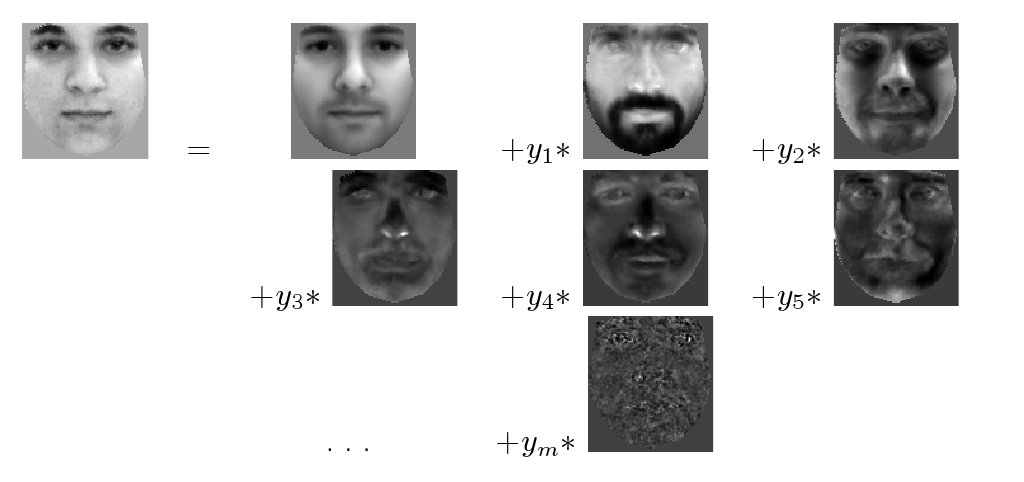
\includegraphics[scale=0.5]{images/eigenfaces_comb_from_nn_vienna.png}
\caption{ Using the eigenfaces we can represent an image as a linear combination of the
  eigenfaces. Taken from \cite{vienna} }
\label{gr:eigenfaces}
\end{figure}

The weight of each eigenface in the linear combination is computed from the
projection of the face image onto this eigenface. To recognize a face we
 first calculate these weights. Then we calculate the Euclidean distance of the vector
of weights to the weights of faces from our training data set. The face from
the data set with weights which are closest to the new image's weights is chosen
as a match.

In an image of 256 by 256 we have a 65,536 dimensional vector that
represents the face image. This means we would require 65,536 eigenfaces to be
able to exactly represent every face. However, images of faces are very similar
in their configuration which means that the underlying principal subspace of
faces has a lower dimension than 65,536. To reduce the dimensionality, PCA is
performed to identify the subset of eigenfaces which span a lower dimensional principal
subspace. Using this subset of eigenfaces, which are called the principal
eigenfaces, we can effectively encode a 65,536 dimensional face image vector using a vector of much smaller
dimensions.

The drawback of a PCA based model is that the recognition rate drops significantly once
independent sources of variation are introduced. Turk and
Pentland noted that the eigenfaces approach has issues with variations in lighting,
head size, head orientation or faces exhibiting expressions \cite{eigenfaces91}. Likewise, when
faces are partially occluded in images it causes difficulties to the technique. 

The eigenfaces approach is based heavily information and coding theory. As
explained, the PCA makes it possible to encapsulate a face image
using low dimensional vector. As such PCA is often used to
reduce dimensionality in more sophisticated modeling approaches.

\subsubsection{Morphable Model}
Blanz et al use PCA to construct a statistical model of 3D face shape and
texture \cite{blanz1}, \cite{blanz2}. The orthogonal matrix of basis vectors is
extracted from a database of 3D faces with texture. This basis spans a vector
space which Blanz refers to as the \textit{Morphable Model}.

The faces in the database are encode as shape vectors with $S_i$ to being the vector representing the 3D shape of a human
face, stored as the $x,y,z$-coordinates of all the vertices of that face. So

\begin{equation}
\mathbf{S_i} = (x_1,y_1,z_1,x_2,...,x_n,y_n,z_n)^T
\end{equation}

Similarly, the texture vectors are defined as

\begin{equation}
\mathbf{T_i} = (R_1,G_1,B_1,R_2,...,R_n,G_n,B_n)^T
\end{equation}

The idea behind the morphable model is that linear combination of the
$\mathbf{S_i}$ and $\mathbf{T_i}$, which is within $\pm 3$ standard deviations
from the mean, constitutes a realistic face. The full
morphable model is the linear combination of the examples given by the formula

\begin{equation}
\mathbf{S} = \sum_{i=1}^Na_i \mathbf{S_i} \indent \mathbf{T} = \sum_{i=1}^Nb_i \mathbf{T_i}
\end{equation}

Blanz et al also performed a Principal Component Analysis (PCA) on the dataset of examples
to produce orthogonal basis vectors that can be used in the morphable
model instead of the examples directly. This reduces the dimensionality of the
model. The eigenvectors given by $\mathbf{s_i}$ and $\mathbf{t_i}$ can be used
to generate new faces as follows

\begin{equation}\label{eq:morhpable_pca}
\mathbf{S} = \mathbf{\bar{s}} + \sum_{i=1}^m\alpha_i.\mathbf{s_i} \indent \mathbf{T} = \mathbf{\bar{t}} + \sum_{i=1}^m\beta_i.\mathbf{t_i}
\end{equation}
where $\mathbf{\bar{s}}$, $\mathbf{\bar{t}}$ are the means of the shape and
texture data and $m < N$. The parameters $\alpha_i$ and $\beta_i$ are the
shape and texture parameters controlling the deformable model.

The PCA process identifies vectors which represent the most variance in
the examples and as such contain the most information about
the images. This means any image can now be represented by the linear
combination of a smaller number of these components than would be
required of the original examples. The linear combination is controlled by the
parameters of the deformable model. This is in essence the eigenfaces modeling approach
only now applied to 3D shapes and textures.

The shape vector and texture vector encode the location and texture values at
specific feature (landmark) points. Therefore, to allow the morphable model to fit to the source image, a
point-to-point correspondence must be ensured on the example
images, so that important features such as the tip of the nose are
correctly matched up in the examples. During the recognition process the features in the source image are matched to those in the examples, in order to
calculate the correct combinations of the basis vectors. According to Blanz, to fit the Morphable Model of 3D faces to an image, the user has to manually select
about 7 feature points. 

\begin{comment}
\subsubsection{3D Reconstruction algorithm}
%Pose and lighting etc in case of exchanging faces
To be able to exchange the face need the $\alpha_i$, $\beta_i$ parameters
of the Morphable Model. We also need 22 rendering parameters
$\rho$ to be able to apply standard graphics procedures to correctly illuminate and position the 3D source face into
the target image. The $\rho$ parameters are:
\begin{multicols}{2}
\begin{itemize}
\setlength{\itemsep}{0pt}
\item 3D rotation (3 angles)
\item 3D translation (3 dimensions)
\item focal length of the camera
\item angle of directed light (2 parameters)
\item intensity of directed light (3 colors)
\end{itemize}
\begin{itemize}
\setlength{\itemsep}{0pt}
\item intensity of ambient light (3 colors)
\item color contrast
\item gain in each color channel (3 channels)
\item offset in each color channel
\end{itemize}
\end{multicols}
We apply the reconstruction algorithm to estimate the parameters for both images
and then use these parameters to compute
the color image $I_{model}(x,y)$ of the face we are reconstructing.

The parameters are all
estimated in an analysis-by-synthesis stage in which we attempt to minimize the
difference between the synthetic image $I_{model}$ and the original color
image $I_{input}$. We measure the quality of this minimization based on a sum of squared error\\
\begin{equation}
E_l = \sum_x \sum_y \sum_{c\in\{r,g,b\}}(I_{c,input}(x,y) - I_{c,model}(x,y))^2
\end{equation}
To this cost error we add another term $E_F$ that measures the plausibility of the
$\rho$ parameters based on a user provided set of 2D feature points. The
resulting cost function that we minimize during the fitting stage is
\begin{equation}
E = \frac{1}{\sigma_l^2}E_l + \frac{1}{\sigma_F^2}E_F + \sum_i
\frac{\alpha_i^2}{\sigma_{S,i}^2} + \sum_i \frac{\beta_i^2}{\sigma_{T,i}^2}
+\sum_i \frac{(\rho_i- \bar{\rho}_i)^2}{\sigma_{R,i}^2}
\end{equation}
where our standard deviations $\sigma$ are taken from the PCA.
This cost function is minimized using a Stochastic Newton Algorithm to
obtain a plausible result for the parameters.

However, there are skin features like moles or scars that we cannot compute from
the linear combinations of the textures $T_i$. Therefore we additionally extract the
texture of the person's face using an
illumination-corrected texture extraction algorithm.
\end{comment}


\subsubsection{Combined Models of Shape and Appearance !ALTERED}
Texture variations and shape variations are correlated. Clearly, with any source of
lighting it is the shape of an object which influences what parts of the object
will appear darker or lighter. Cootes and Taylor \cite{activeApp04} describe modeling approaches
which account for the correlations between the two sources of
variation can be modeled. The models they introduce are well suited for highly
variable structures such as faces or internal organs. Using PCA based shape and
texture models, Cootes and Taylor construct Active
Shape and Active Appearance Models which, despite the name, are model fitting algorithms that find the parameters statistical models to fit instances of objects in images.

The shape model are constructed by annotating feature points in
images, collecting these into a data matrix and then performing PCA on the
covariance matrix of this data to generate a lower dimensional basis
$\mathbf{P}_s$. The shape model then makes it possible to synthesize new shapes
as follows
\begin{equation}\label{eq:shape}
\mathbf{S} = \mathbf{\bar{s}} + \mathbf{P}_s\mathbf{b_s}
\end{equation}
To construct the texture model, the image is first warped into the mean shape
$\bar{s}$ to obtain a ``shape-free'' image. The gray-scale values at points in
the shape-free which correspond to feature points in the mean shape are then
measured and combined into a texture data matrix. Then PCA is used to find
eingenvector matrix $\mathbf{P}_t$. This matrix of eigenvectors gives the
linear model for texture as
\begin{equation}\label{eq:text}
\mathbf{T} = \mathbf{\bar{t}} + \mathbf{P}_t\mathbf{b_t}
\end{equation}

So similarly to the approach of Blanz as seen in formula \ref{eq:morhpable_pca}, Cootes and Taylor separate the shape and the information of a target image into
two distinct vectors -- the shape parameter vector $\mathbf{b_s}$ and the texture
represented by the grey-level vector $\mathbf{b_t}$ (here the image is
gray-scaled). To obtain a model which addresses both shape and texture, these
parameter vectors are combined into one vector $\mathbf{b} = [\mathbf{b_s}\, \mathbf{b_t}]^T$. Then PCA is applied to this combined vector to get an
eigenvector basis $\mathbf{P_c} =
\bigl( \begin{smallmatrix}P_cs\\P_ct\end{smallmatrix} \bigr)$ for the parameters $\mathbf{b_s}$ and
$\mathbf{b_t}$. This new basis encapsulates the correlation between shape and
texture, thus making it possible to express the other
parameters as functions of a parameter vector $\mathbf{c}$ as follows
\begin{align} \label{gth:shape_mod} 
\mathbf{S} &= \mathbf{\bar{s}} + \mathbf{P}_s \mathbf{W}_s^{-1} \mathbf{P}_{cs}c\\
\label{gth:texture_mod}
\mathbf{T} &= \mathbf{\bar{t}} + \mathbf{P}_t \mathbf{P}_{ct} \mathbf{c}
\end{align}
where $\mathbf{W}_s$ is a diagonal matrix of weights which allows the shape and
texture models to have different units. To reconstruct a new face using the model we first determine the $\mathbf{b_s}$ and
$\mathbf{b_g}$ parameters from the new face image. These parameters are then
used to calculate the $c$ using by projecting them using the eigenvector basis
as $\mathbf{c} = \mathbf{P_c}^T\mathbf{b}$.

\paragraph{Active Shape Model.}
The Active Shape model (ASM) proposed by Cootes and Taylor is model fitting
algorithm based
on the statistical models of shape and texture. The ASM enables us to locate a
shape in an image using an iterative
procedure as shown in figure \ref{gr:asm}. To search for objects in an image
using the ASM, we first place the shape model, which we obtained from the training data, into
the center of the image. In the next iterations a texture profile of $k$
neighboring points around each point of the shape model is taken and compared
with the texture profile of this point obtained when training the model. Then
the point of the shape model is moved to make the difference between the two
profiles smaller. This process is repeated until convergence is reached.

\begin{figure}[H]
\centering
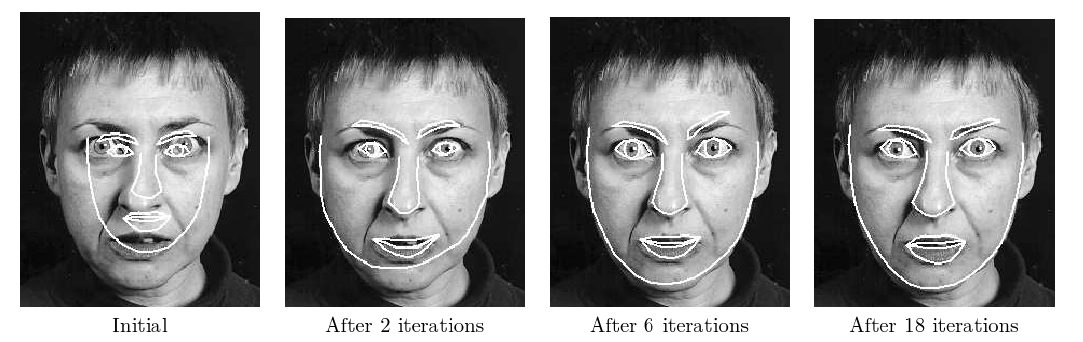
\includegraphics[scale=0.5]{images/scary_face2.png}
\caption{ Active Shape Model iterations shown on finding the shape of a
  previously unseen face. Taken from \cite{cootesOverview01} }
\label{gr:asm}
\end{figure}

The ASM moves the point only based on the texture profile of a
local neighborhood of this point. The obvious problem with this approach is
that it is a local search technique and thus it depends too much on the choice of the
starting point. If the target image is not centered on the face and the
algorithm begins in the center of the image, then it can possibly converge on incorrect
shapes such as the nose as can be seen in figure \ref{gr:bad_asm}. This is due to
the fact that as a local search method, the ASM cannot escape a local minimum.

\begin{figure}[H]
\centering
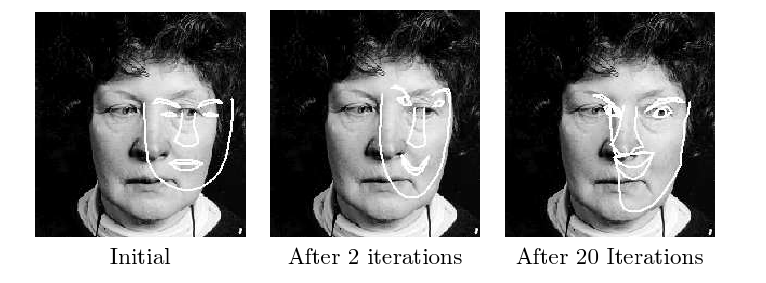
\includegraphics[scale=0.7]{images/bad_asm.png}
\caption{ Incorrect convergence of the ASM when the search is initialized
  incorrectly. This can happen when the face is not centered in the image or
  when the search does not begin in the center of the image. Taken from \cite{cootesOverview01} }
\label{gr:bad_asm}
\end{figure}

To improve the efficiency and the robustness of ASM, Cootes
suggests performing several searches at different resolution. First a coarse
search is performed on the image with a low resolution until the search converges. The resulting configuration
of the shape model points from this coarse search
then serves as the starting point for a search in the same image with a better
resolution. The advantage of adopting this coarse to fine search approach is
that it makes the search less susceptible to converging on incorrect shapes. When
searching at a lower resolutions it will be easier to find the outlines of the
face. Once the search is restarted with a higher resolution, shapes like the
mouth and the nose can be identified.

\paragraph{Active Appearance Model.}
The Active Appearance Model (AAM) is a model fitting technique based on a
combined shape and texture model defined by equations \ref{gth:shape_mod} and \ref{gth:texture_mod}. The AAM enhances the Active Shape model search by also considering the texture
information in the entire object.

The AAM search attempts to minimize the difference between the texture (the
grey-levels) of the image we are searching and the grey-levels of the
image generated with the current model parameters. The difference vector which
 is minimized every iteration is defined as:
\begin{equation}
\delta \mathbf{I} = \mathbf{I}_i - \mathbf{I}_m
\end{equation}
where $\mathbf{I}_m$ is the vector of the grey-levels generated with the current model
parameters and $\mathbf{I}_i$ is a vector containing the grey-levels of the
image. The goal of AAM is to minimize the difference $\delta \mathbf{I}$ between
the synthesized and observed grey-levels.

To simplify this optimization problem, Cootes and Taylor propose to allow the
computer to learn the relationship
between the difference vector $\delta \mathbf{I}$ and the error in the model
parameters. Learning this relationship makes it possible to correctly improve the
model for a given measured error in an iterative procedure.

The AAM iterations are depicted in figure \ref{gr:amm}. The process attempts
change model parameters to fit it to an unseen face. This fitting is done by
minimizing the differences between pixels at the landmark points.

\begin{figure}[H]

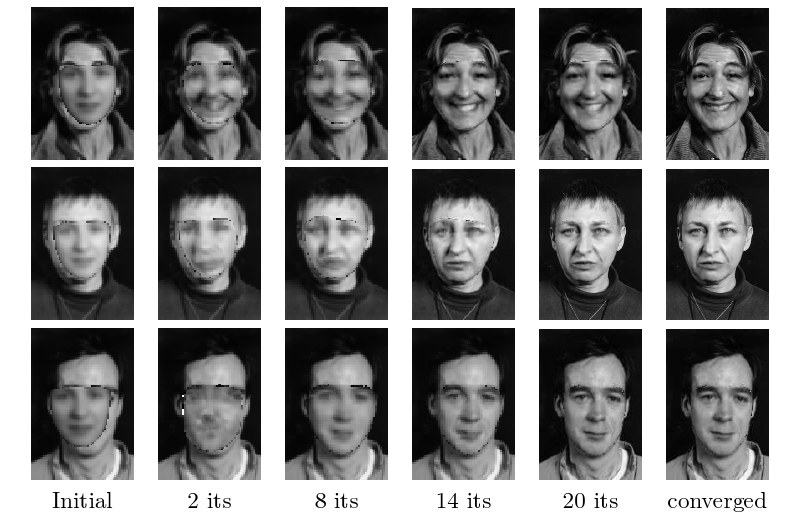
\includegraphics[scale=0.7]{images/amm_example.png}
\caption{ Active Appearance Model iterations shown when searching for previously
 unseen faces. Taken from \cite{activeApp04} }
\label{gr:amm}
\end{figure}

The drawback of both the ASM and AAM search is that it is required of the user to specify
landmark points on the target image. This means the technique is not well suited
for applications where the model would have to be matched to a large number of
faces. To combat this problem, a number of automatic 2D and 3D landmark location
solutions can be used \cite{activeApp04}.

Another problem of both the ASM and the AAM lies in the fact that they do not
distinguish or model the individual factors responsible for shape or texture
variation. They only acknowledge two sources of variation in the image. In the
case of face models, this means that variation caused by
identity and the variation caused by expression are not perceived as two
fundamentally different sources. Thus, it is impossible to only alter one
variational source while leaving the other source constant. This makes the
models unsuitable for expression transfer.

\subsection{Tensor Models}
Vasilescu and Terzopoulos \cite{Ter1}, \cite{Ter2}, \cite{Ter3} defined a
generalization of statistical methods using multilinear algebra. Statistical
analysis of images using PCA determine the variation of the training
dataset. The drawback of the PCA is that it only addresses one factor -- one
source of variance in the images. All variation is explained using the
orthogonal eigenvectors and the eigenvalues. With images of faces, the PCA
approach works well when only the identity or only the expression varies. Using
methods of multilinear analysis it is possible to model the interaction of
several sources of variation.

The multilinear approach has mostly replaced the PCA method and will be also used in the
expression transfer application we develop. Here we will go over an overview of
multilinear algebra to elucidate the advantages of multilinear
models. Details concerning design and implementation specifics of the tensor
based model will be covered
in chapter \ref{design}. A comprehensive discussion of multilinear algebra and
its application was compiled by De Lathauwer in \cite{multilinear}. Detailed
discussion of matrix calculations and matrix calculus can be found in \cite{matcalc}, \cite{matrix}, \cite{kronecker}.

\subsubsection{Multilinear Algebra}
Multilinear algebra is based on the generalization of matrix
operations. Matrices are linear operators and can be seen as linear functions
defined over vector spaces. In multilinear algebra the operators are
\textit{tensors}. 

\paragraph{Tensors.} In multilinear algebra tensors
define multilinear operators over a set of vector
spaces. Tensors are organized into mode spaces. The $N$-mode tensor contains $N$
mode spaces and each item of data contained in the tensor is indexed by $N$
values. The number of modes determines the order of a tensor, so an $N$-mode tensor has order $N$. If
$\mathcal{A}$ is a tensor of
order $N$, then $\mathcal{A} \in \mathbb{R}^{I_1 \times I_2 \times \ldots \times
  I_N}$ where $I_i$ are the mode spaces. Vectors are 1$^{st}$ order tensors, matrices are 2$^{nd}$ order
tensors. In a matrix the first mode space is the row space, the $2$-mode space
is the column space.

\paragraph{Tensor Flattening.} Any tensor can be flattened into a matrix. Tensor
flattening (or matrix unfolding) is defined as follows; given
an $N$th-order tensor $\mathcal{A} \in \mathbb{R}^{I_1 \times I_2 \times \ldots
  \times I_N}$, this tensor can be flattened along mode $i \in
\{1,2,\ldots,N\}$ to give $\mathbf{A_{(i)}} \in \mathbb{R}^{I_i \times I_1 I_2 \ldots I_{i-1} I_{i+1} \ldots I_N}$. 

The flattening corresponds to aligning the vectors from the mode space $i$ into a matrix. To illustrate tensor flattening lets define the 3$^{rd}$ order
  tensor $\mathcal{B} \in \mathbb{R}^{3\times 2\times 3}$ by $b_{111} = b_{112}
  = b_{113} = b_{211} = b_{123} = -b_{212} = -b_{313} = 1$, $b_{311} = b_{122} =
  b_{322} = b_{323} = -b_{213} = -b_{222} = 2$, $b_{312} = 0$, $b_{121} =
  b_{221} = 4$ and $b_{223} = -5$. Then tensor flattening along mode $1$ is given by

\begin{align*}
\mathbf{B_{(1)}} = 
\begin{pmatrix}[ccc|ccc]
1&1&1&4&2&1\\
1&-1&-2&4&-2&-5\\
2&0&-1&2&2&2
\end{pmatrix}
\end{align*}
The flattening along mode $2$ are the vectors along the second mode space
\begin{align*}
\mathbf{B_{(2)}} = 
\begin{pmatrix}[ccc|ccc|ccc]
1&1&2&1&-1&0&1&-2&-1\\
4&4&2&2&-2&2&1&-5&2
\end{pmatrix}
\end{align*}
Tensor flattening is useful since it makes it possible to express tensor
operations using matrices. The schema for flattening a 3$^{rd}$ order tensor is shown in figure \ref{fg:flat}

\begin{figure}[H]
\centering
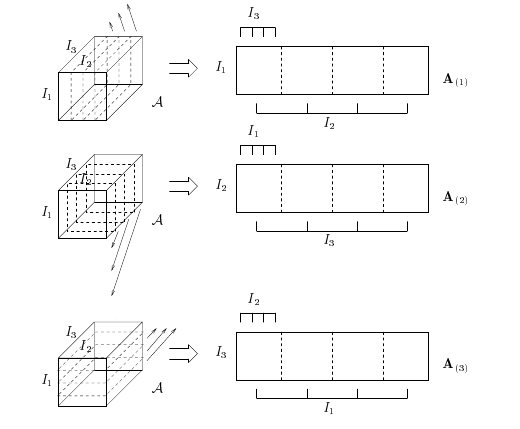
\includegraphics[scale=0.75]{images/flattening3.png}
\caption{ Flattening of the $(I_1\times I_2 \times I_3)$-tensor $\mathcal{A}$
into three matrices; the $(I_1\times I_2 I_3)$-matrix $\mathbf{A_{(1)}}$,
the $(I_2\times I_3 I_1)$-matrix $\mathbf{A_{(2)}}$ and the $(I_3\times I_1 I_2)$-matrix $\mathbf{A_{(3)}}$. Taken from \cite{multilinear}.}
\label{fg:flat}
\end{figure}

\paragraph{Kronecker product.} The Kronecker Product between a $m \times n$
matrix $A$ and a $p \times q$ matrix $B$ is a $(mp) \times (nq)$ matrix defined
as
\begin{equation}\label{eq:kronecker}
A \otimes B = 
\begin{pmatrix}
a_{11}B & a_{12}B & \ldots & a_{1n}B\\
a_{21}B & a_{22}B & \ldots & a_{2n}B\\
\vdots& & &\\
a_{m1}B & a_{m2}B & \ldots & a_{mn}B
\end{pmatrix}
\end{equation}

\subparagraph{Properties.}The Kronecker product possesses a number of useful properties. First the
connection between matrix product and kronecker product is given by
\begin{equation}\label{eq:kron_mult}
(A \otimes B)(C \otimes D) = (AC \otimes BD)
\end{equation}
where $A$ is a $m \times n$ matrix, $B$ a $p \times q$ matrix, $C$ a $n \times
r$ matrix and $D$ a $q \times s$ matrix.

\subparagraph{Proof.} The proof comes from block multiplication of the two Kronecker products as
follows
\begin{align*}\label{}
(A \otimes B)(C \otimes D) &= 
\begin{pmatrix}
a_{11}B & a_{12}B & \ldots & a_{1n}B\\
a_{21}B & a_{22}B & \ldots & a_{2n}B\\
\vdots& & &\\
a_{m1}B & a_{m2}B & \ldots & a_{mn}B
\end{pmatrix}
\begin{pmatrix}
c_{11}D & c_{12}D & \ldots & c_{1r}D\\
c_{21}D & c_{22}D & \ldots & c_{2r}D\\
\vdots& & &\\
c_{n1}D & c_{n2}D & \ldots & c_{nr}D
\end{pmatrix}\\
&=\begin{pmatrix}
(\sum_{j=1}^n a_{1j}c_{j1})DB & (\sum_{j=1}^n a_{1j}c_{j2})DB & \ldots &
  (\sum_{j=1}^n a_{1j}c_{jr})DB\\ 
(\sum_{j=1}^n a_{2j}c_{j1})DB & (\sum_{j=1}^n a_{2j}c_{j2})DB & \ldots & (\sum_{j=1}^n a_{2j}c_{jr})DB\\ 
\vdots&  &\\
(\sum_{j=1}^n a_{mj}c_{j1})DB & (\sum_{j=1}^n a_{mj}c_{j2})DB & \ldots & (\sum_{j=1}^n a_{mj}c_{jr})DB\\ 
\end{pmatrix}\\
&= (AC \otimes BD)
\end{align*}

\begin{comment}
&\begin{pmatrix}
a_{11}Bc_{11}D + a_{12}Bc_{21}D + \ldots + a_{1n}Bc_{n1}D & \ldots & a_{11}Bc_{1r}D + a_{12}Bc_{2r}D + \ldots + a_{1n}Bc_{nr}D\\
\vdots&  &\\
a_{m1}Bc_{11}D + a_{m2}Bc_{21}D + \ldots + a_{mn}Bc_{n1}D & \ldots & a_{m1}Bc_{1r}D + a_{m2}Bc_{2r}D + \ldots + a_{mn}Bc_{nr}D
\end{pmatrix}
=\\
\end{comment}

The transpose of the Kronecker product is the transpose of the component
matrices.
\begin{equation}\label{eq:krontran}
(A \otimes B)^T = A^T \otimes B^T
\end{equation}

\subparagraph{Proof.} The proof can be seen from block transposing the Kronecker product.
\begin{align*}
(A \otimes B)^T &=
\begin{pmatrix} 
a_{11}B & \ldots & a_{1n}B\\
a_{21}B & \ldots & a_{2n}B\\
\vdots&  &\\
a_{m1}B & \ldots & a_{mn}B
\end{pmatrix}^T
=\begin{pmatrix}
a_{11}B^T  \ldots & a_{m1}B^T\\
a_{12}B^T  \ldots & a_{m2}B^T\\
\vdots& \\
a_{1n}B^T  \ldots & a_{mn}B^T
\end{pmatrix}
= A^T \otimes B^T
\end{align*}

If the matrices $A$ and $B$ are invertible then the Kronecker product is
invertible as well. The inverse of the Kronecker product is given by
\begin{equation}\label{eq:kron_inv}
(A \otimes B)^{-1} = A^{-1} \otimes B^{-1}
\end{equation}
\subparagraph{Proof.} The inverse formula is derived from property
\ref{eq:kron_mult}.
\begin{align*}
(AA^{-1} \otimes BB^{-1}) = (A \otimes B)(A^{-1} \otimes B^{-1}) = I
\end{align*}
thus $(A^{-1} \otimes B^{-1})$ is the inverse of the Kronecker product.

From \ref{eq:kron_mult} and \ref{eq:krontran} we can see that the Kronecker product of two orthogonal matrices is again orthogonal.
\begin{align}\label{eq:kron_ortho}
(A \otimes B)^T(A \otimes B) = (A^T \otimes B^T)(A \otimes B) = (A^TA \otimes
  B^TB) = (I \otimes I) = I
\end{align}
and similarly to show for $(A \otimes B)(A \otimes B)^T = I$.
\paragraph{Frobenius Norm.} The Frobenius-norm of a tensor is a measure of the
size of the tensor. It is defined as
\begin{equation}\label{eq:frob}
\lVert \mathcal{A} \rVert = \sqrt{ \sum_{i_1} \sum_{i_2} \ldots \sum_{i_N}
  a_{i_1 i_2 \ldots i_N}^2 }
\end{equation}
Thus the Frobenius norm is merely the sum over the square of all elements. For matrices the Frobenius norm simplifies to a square root of the
trace of the squared matrix.

\paragraph{Mode-$n$ product.}
The mode spaces of
a tensor can be altered independently of the other
mode spaces by a linear transformations called \textit{mode-$n$ product}. The
mode-$n$ product is defined between a matrix $\mathbf{M}$ and a tensor
$\mathcal{A}$ with the result being another tensor $\mathcal{B}$. The product is
written as $\mathcal{B} = \mathcal{A} \times_n \mathbf{M}$. The mode-$n$ product
by the matrix $\mathbf{M}$ transforms all the vectors $\mathbf{v}$ in the $n$-th mode of the tensor into vectors
$\mathbf{M}\mathbf{v}$. It is therefore possible to separately transform the vectors in
mode-$3$ and the vectors in mode-$2$. The mode-$n$ product can also be expressed in
terms of flattened matrices as $\mathbf{B}_{(n)} = \mathbf{M} \mathbf{A}_{(n)}
$. We can therefore rewrite the singular value decomposition (SVD) of a matrix $\mathbf{D
  = U\Sigma V^T}$ using the mode-$n$ product as $\mathbf{D} = \mathbf{\Sigma} \times_1
\mathbf{U} \times_2 \mathbf{V}$. 

The successive application of $N$ mode-$n$ products to a tensor can be
represented using flattened tensors, matrix products and Kronecker products as follows
\begin{align}\label{eq:modemult}
\mathcal{B} &= \mathcal{A} \times_1 \mathbf{M}_1 \times_2 \mathbf{M}_2  \ldots
\times_n \mathbf{M}_1n \ldots \times_N \mathbf{M}_N\\
\label{eq:kronmodemult}
\mathbf{B}_{(n)} &= \mathbf{M}_n \mathbf{A}_{(n)} (\mathbf{M}_{n-1} \otimes
\mathbf{M}_{n-2} \otimes \ldots \mathbf{M}_1 \otimes \mathbf{M}_N \otimes \ldots \mathbf{M}_n+1)^T 
\end{align}
Equation \ref{eq:modemult} shows the application of $N$ mode-$n$
products. In equation \ref{eq:kronmodemult} the equivalent formulation is given
using matrices instead of tensors. Note that the transpose can be brought into
the parentheses in the second term of
\ref{eq:kronmodemult}, due to the transpose property of
the Kronecker product \ref{eq:krontran}. The order of the matrices inside of the
parentheses is important. If this order is changed than the result has the
same columns but in a different order.
\paragraph{High Order Singular Value Decomposition (HOSVD).}

The \textit{N-Mode singular value decomposition} (or high order SVD) is a linear
transformation of a tensor. An $N$-order tensor has $N$ mode spaces. The high
order SVD orthogonalizes the mode spaces by finding the $N$ sets of orthonormal basis vectors
which span the column space along the respective mode space. The HOSVD
decomposition is as follows \cite{multilinear}
\begin{equation}\label{eq:HOSVD}
\mathcal{A} = \mathcal{S} \times_1 \mathbf{U}_1 \times_2
\mathbf{U}_2 \times_3 \mathbf{U}_3 \dotsb \times_N \mathbf{U}_N
\end{equation}

Equation \ref{eq:HOSVD} decomposes the tensor into a \textit{core
  tensor} $\mathcal{S}$ and orthonormal mode matrices $\mathbf{U}_1 \ldots
\mathbf{U}_N$. The mode matrix $\mathbf{U}_i$ contains the orthonormal vectors
$u_ij$ which form the orthogonal basis of the column space of the flattened
tensor $\mathbf{A}_{(n)}$. The core tensor governs the interaction between these
mode matrices and is as such analogous to a diagonal matrix of eigenvalues used
in PCA. Eigenvalues can be seen as measures of the variance along the
corresponding eigenvector directions. However, the core tensor does not have a
diagonal structure. Rather it has the property of all-orthogonality whereby all
subtensors of $\mathcal{S}$, obtained by fixing one index, are orthogonal. The
Forbenius norms of these subtensors decrease, which makes it possible to reduce the dimensionality of
the data set by truncating the core tensor. It is therefore possible to
approximate the original tensor using a reduced core tensor. The approximation
of a tensor
$\mathcal{A}$ using a reduced core tensor $\mathcal{S}_{reduced}$ is derived from the
mode-n SVD and is defined as:
\begin{equation} \label{eq:core_tensor}
\mathcal{A} \approx \mathcal{S}_{reduced} \times_1 \hat{\mathbf{U}}_1 \times_2
\hat{\mathbf{U}}_2 \times_3 \hat{\mathbf{U}}_3 \dotsb \times_N \hat{\mathbf{U}}_N
\end{equation}
The matrices $\hat{\mathbf{U}}_i$ are truncated versions of the eigenvector
matrices for the corresponding mode space. Figure \ref{fg:hosvd} depicts the
approximate HOSVD using the truncated core tensor and mode matrices.

\begin{figure}[H]
\centering
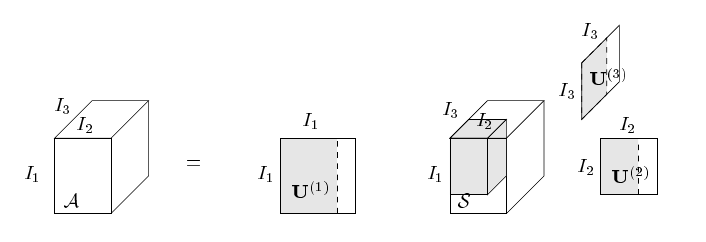
\includegraphics[scale=0.755]{images/n_mode_svd2.png}
\caption{Multilinear face model showing how different attributes change along
  the modes. Taken from \cite{multilinear} }
\label{fg:hosvd}
\end{figure}

\paragraph{HOSVD Algorithm.} The HOSVD decomposition of a tensor $\mathcal{A}$
of order $N$ is computed as follows:
\begin{itemize}
\item \textbf{Step 1}. For $i=1,\ldots,N$ compute the mode matrix $\mathbf{U}_i$
  by calculating the SVD of the flattened matrix $\mathbf{D}_{(i)} = \mathbf{U_i
    \Sigma_i V_i^T}$. The left singular matrix of $\mathbf{D}_{(i)}$ is the mode
  matrix for mode $i$.
\item  \textbf{Step 2}. Compute the core tensor by reversing equation
  \ref{eq:HOSVD} to get the core tensor as 
\begin{equation}\label{eq:core}
\mathcal{S} = \mathcal{A} \times_1 \mathbf{U}_1^T \times_2
\mathbf{U}_2^T \times_3 \mathbf{U}_3^T \dotsb \times_N \mathbf{U}_N^T
\end{equation}
\end{itemize}


\subsubsection{Tensor-Based Model}\label{works}
The possibility of using a multilinear approach to construct face models was explored
by numerous researchers. Vasilescu and Terzopoulos \cite{Ter1} build a tensor from a
database of face images and construct \textit{tensorfaces} by performing HOSVD
on the data tensor. Tensorfaces are contained as vector the mode matrices
$\mathbf{U}_i$. Vlasic, Brand, Pfister and Popovic \cite{faceTransfer05} build a
tensor model of 3D faces an utilize it to recognize faces in video sequences for
the purpose of expression transfer. The group
successfully managed to implemented a face transfer application based on a
multilinear face model which allowed for expressions and even for speech related
movements to be transferred between video-recordings of two different subjects. The multilinear
model was estimated from geometric variations in 3D face scans that Vlasic and
his group collected. Two tensor models with different dimensionality were utilized. Their first model was a lower dimensional bilinear model that organized the data into three
groups of vertices, identity and expression. Their higher dimensional model
organized faces into groups of expressions, vertices, identities and visemes. The parameters for the multilinear face model, which were used to synthesize new expressions, were
extracted from the video input using an optical flow algorithm.

To construct a bilinear face model it is necessary to separate the faces from the
database into groups of expressions and identities in order to organize them
into the tensor. The tensor based approach allows us to organize
the data in a way that makes for easier manipulation with a transformation
matrix. The groups are aligned in the tensor along the modes as shown in figure
\ref{gr:tensor}. In this example the vertices change along the mode-1 space, the identity changes
along the mode-2 space and the expressions change along the mode-3 space. 
\begin{figure}[H]
\centering
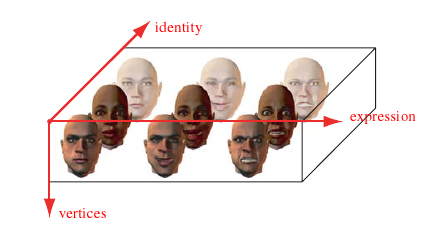
\includegraphics[scale=0.8]{images/modes_faces.png}
\caption{Multilinear face model showing how different attributes change along
  the modes. Taken from \cite{faceTransfer05} }
\label{gr:tensor}
\end{figure}


Vlasic et al constructed a multilinear
face model using mode-n SVD and decomposing the organized tensor into mode
matrices. A generative model can be constructed when the core tensor and the the
mode-$1$ matrix are combined together using the mode-$n$ product. The first mode
space which holds the vertices, which the model should be capable of generating. Using equation \ref{eq:core_tensor} the
data tensor $\mathcal{D}$ is decomposed as
\begin{equation} \label{eq:multilin_face}
\mathcal{D} \approx \mathcal{M} \times_2
\hat{\mathbf{U}}_2 \times_3 \hat{\mathbf{U}}_3 \dotsb \times_N \hat{\mathbf{U}}_N
\end{equation}
where tensor $\mathcal{M}$ is called the \textit{multilinear model}. The
multilinear model can then be used to synthesize new faces. Mode multiplying the
multilinear model with one row from
each mode matrix we recover exactly one of the original faces. Mode multiplying
the model $\mathcal{M}$ with a linear combination of rows from the truncated
mode matrices synthesizes a new face $\mathbf{f}$ giving us the generative
tensor model as
\begin{equation} \label{eq:generative_model}
\mathbf{f} = \mathcal{M} \times_2
\mathbf{w}_{2}^T \times_3 \mathbf{w}_3^T \dotsb \times_N \mathbf{w}_N^T
\end{equation}
The weight vectors $\mathbf{w}_{2}, \ldots ,\mathbf{w}_{N}$ are column vectors
which encode the attribute of the corresponding mode space.

The tensor-based model is
similar to what we saw in the eigenfaces PCA approach in figure
\ref{gr:eigenfaces}. However, the tensor-based approach has the advantage that
we can manipulate the different sources of variance (i.e. in the case of a face
model the identity, the
expressions) separately. This advantage outweighs the additional computational
complexity carried by the high order SVD and makes this model suitable for the
task of expression transfer.

The drawback of the method described by Vlasic et al is that it requires the
tensor to be fully populated. This means that we require all
expressions to be performed by all subjects to have a full tensor. This raises
issues when some data is corrupted or lost during data gathering. There are two
ways of coping with this problem. The first approach is to use a
statistical method to model the data. Alternatively the missing data can be estimated from the current data.
\subsubsection{Tensor-based Statistical Discriminant Method}
The tensor-based statistical discriminant methods (SDM) was successfully used by Minoi and Gillies
\cite{sdm,jacey} to synthesize expressions and to neutralize faces displaying an
expression. The SDM is based on Fischer's linear discriminant analysis (LDA) \cite{lda}. The LDA
differs from the standard PCA eigenfaces approach in that it seeks to separate
data into distinct classes. The way this is done is by projecting the data into
a lower dimensional subspace that maximizes the between class separability and
minimizes the within class variance.

In LDA we first separate the training data set into a number of groups. Then we
look for the between class scatter matrix $S_b$ and the within class scatter
matrix $S_w$. The matrix $\Phi_{lda}$ that defines the projection onto the desired low dimensional
space is defined as:
\begin{equation} \label{eq:lda}
\Phi_{lda} = \textrm{arg} \max_{\Phi}\frac{\lvert \Phi^T S_b \Phi \rvert}{\lvert \Phi^T S_w \Phi \rvert}
\end{equation}
In equation \ref{eq:lda} the ratio of the determinant of the between class
separability and the determinant of the within class variability is
maximized. The maximum of this equation is the optimal projection.

However, the LDA approach has difficulties when the training data set is small
in comparison to the dimensions of the image. This is called the \textit{small
sample size problem} and it causes the scatter matrices to be singular when the
number of data items is less than the number of variables. To overcome the small size problem the statistical discriminant method can be used.

The SDM approach consists of two stages. In the first stage the PCA
and LDA are used to reduce the dimensionality and find the discriminant
directions of the classes. The PCA helps to overcome the small size problem
common to stand-alone LDA. In the second stage the most discriminant vectors of
our classes are projected back into the original high dimensional space. This
back projection will give us a vector for every class in the high dimensional
space. These vectors allow us to synthesize an expression for a new face image by moving the the surface
points of this new image in the direction of one of the vectors. 

The SDM technique can be extended to tensor models by expanding the mode
responsible for expressions into a number of modes representing
individual expression classes, thereby effectively increasing the dimension of
the tensor. The expanded tensor model still retains the quality of independence
along the modes of variance. However, due to the expansion the SDM can be
applied to the tensor if we flatten the sub-tensors into matrices.

\section{3D Pose Estimation}\label{s:3dpose}
The goal of 3D pose estimation is to determine the position and orientation of
an object from a 2D image of the object. A special case of 3D pose estimation is
the \textit{Perspective-n-Point} (PnP) problem. This class of problems is specified as follows -
given are the exact locations of a set of feature points on the object and the
positions of points in the 2D
image. The points in the 2D image correspond to the 3D feature points. The goal
is to find how the object must be moved, rotated, scaled so that when the
3D feature points are projected using a camera model the result will approximate
the input set of corresponding 2D points.  

\subsection{Camera Model}\label{s:camera}
The camera model describes a \textit{projective transformation}. This transformation maps a 3D
point $\mathbf{X} = (X,Y,Z)^T$ to a 2D image point $\mathbf{x} = (x,y)^T$. The
three most important camera models are the perspective model, the orthogonal
model and the weak perspective model.


\subsubsection{Perspective Camera Model}
In perspective projection rays coming from points in the scene all enter the \textit{center of
projection}. These points are then ``projected'' onto an imaging surface, the
\textit{image plane}. The size of the image relative to the distant object is given by
the parameter \textit{focal length}. The focal length is the distance of the
center of projection from the image plane. If the image plane is in behind the
center of projection then the image of the object on the image plane is
inverted. If the image plane is placed in front of the center of projection then the image and
the object have the same orientation. The center of projection in essence
corresponds to an ideal pinhole camera. The perspective projection in therefore known as the
pinhole camera model. 

The normal vector to the pinhole plane, which goes through the pinhole itself is
called the \textit{optical axis}. The optical axis is usually chosen either the
negative or positive $z$ axis and the pinhole is chosen to lie at the origin. The intersection of the optical axis and the
image plane is known as the \textit{principal point}. The configuration of the
pinhole camera model is shown in figure \ref{fg:pin}.
\begin{figure}[H] 
\centering
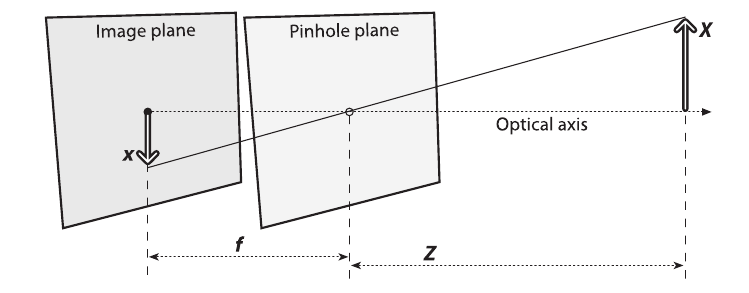
\includegraphics[scale=0.75]{images/pinhole.png}
\caption{Perspective projection camera model with the image plane behind the camera}
\label{fg:pin}
\end{figure}

From figure \ref{fg:pin}, we can see that the image plane is located at $Z=f$
where $f$ is the focal length. The coordinates of the projection of $X$ can
therefore be calculated using similar triangles to obtain $-x/f = X/Z$.
If the image plane were to be place in front of the camera then the ratio given
by the similar triangles will stay the same but the new coordinate will no
longer be negative.

Hence, assuming that the principal point is given by $(c_x,c_y)^T$ and the focal
length is $f$, then the projection $(x,y)^T$ of the point $\mathbf{X} = (X,Y,Z)^T$ is given by
\begin{align}\label{eq:pinCoord}
\begin{pmatrix}x\\y\end{pmatrix} = \frac{f}{Z}\begin{pmatrix}X\\Y\end{pmatrix} + \begin{pmatrix}c_x\\c_y\end{pmatrix}
\end{align}


The perspective projection is a non-linear transformation which cannot be written
as a multiplication of a 3D points in Cartesian coordinates with a matrix. To obtain a matrix formulation, we must
use homogeneous coordinates. The homogeneous coordinates of a point are $P_h =
[p_x,p_y,p_z,s]^T$. The fourth coordinate component $s$ is called
\textit{scale}. We transform a point in homogeneous coordinates into Cartesian
coordinates by dividing the first three components by the scale to get the point
$P_c = [p_x/s, p_y/s, p_z/s]^T$. Using homogeneous coordinates the pin hole
camera model has the form
\begin{equation}\label{eq:projective}
\gamma\begin{pmatrix}x\\y\\1\end{pmatrix}
= \begin{pmatrix}f_x&0&c_x&0\\0&f_y&c_y&0\\0&0&1&0\end{pmatrix} \begin{pmatrix}X\\Y\\Z\\1\end{pmatrix}
\end{equation}
where $\gamma = 1/s$ is responsible for converting the homogeneous result of the
multiplication to Cartesian coordinates. In equation \ref{eq:projective} two
different focal lengths have been used. This is due to the fact that with any
camera equipment the image plane will have dimensions in millimeters. The values
$f_x$ and $f_y$ therefore incorporate the focal length as well as the conversion
from units of the imaging equipment to pixels.

\subsubsection{Orthogonal Camera Model}
In the orthogonal camera model the image of an object is obtained by casting
rays parallel to the optical axis from points $(X,Y,Z)$ on the object and intersecting
these rays with the image plane. The $Z$ component is thereby dropped
entirely. The projected point is thus given by $x = X$ and $y = Y$. The geometry
of the orthogonal projection is shown in figure \ref{fg:weakOrtho}. Orthographic
projection is sometimes called parallel projection, since unlike in perspective
projection, parallel lines remain after being projected into the image plane.

\subsubsection{Weak Perspective Camera Model}\label{s:weak}
The weak perspective camera model is in essence just a scaled orthographic
projection. With this camera model it is possible to approximate a perspective
transformation under the following conditions.
\begin{itemize}
\item The object lies close to the optical axis.
\item The object's depth (the difference between the maximum and minimum $z$ value of the
  object) is small in comparison to the object's average distance from the
  center of projection.
\end{itemize}
Since the depths of the different points on the object are close to each other,
we make the assumption all these depths are equal. Then a perspective projection
of any object point $(X,Y,Z)$ can be approximated as
\begin{equation}
\begin{pmatrix}x\\y\end{pmatrix} = \frac{f}{Z_{avg}}\begin{pmatrix}X\\Y\end{pmatrix}
    + \begin{pmatrix}c_x\\c_y\end{pmatrix}
\end{equation}
where $Z_{avg}$ is the average distance of the object's point from the
camera. Geometrically, we place a plane parallel to the image plane at a
distance $Z_{avg}$ from the center of projection. Then the object points
orthogonally projected onto this new plane. Finally, we perspectively project
these projected points onto the image plane. The geometry of the weak perspective projection is shown in figure \ref{fg:weakOrtho}.

Moreover, the weak perspective transformation is a linear
transformation unlike the strong perspective transformation, since we are
dividing by a constant $Z_{avg}$ and not the $Z$ component of the
point.

\begin{figure}[H] 
\centering
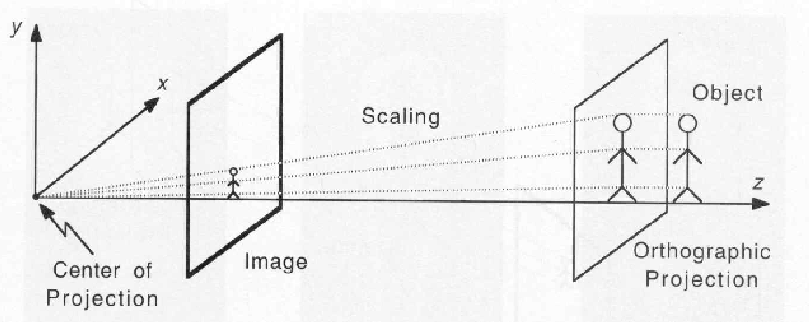
\includegraphics[scale=0.75]{images/weak_persp.png}
\caption{Weak perspective projection is a scaled orthographic projection. The
  image obtained by orthographic projection is scaled by the constant $f/Z_{avg}$.}
\label{fg:weakOrtho}
\end{figure}
  

\subsection{Rotation and Translation}
It is usual in most 3D rendering frameworks to define two coordinate systems. One
coordinate system for the camera and one for the object. This makes it possible
to apply transformations to objects independently since the points that make up each object are defined
in each object's separate coordinate system. A transformation translates the points
from the object coordinate system into the camera coordinate system. In case of $n$ objects there are $n$
independent object coordinate systems thereby making it possible to apply a
different transformation to each of the $n$ object coordinate systems and move
the objects independently which is a crucial task for 3D rendering frameworks.

The transformations of the objects are based on the degrees of freedom for
movement in 3D space. The two classes of transformations are rotation and
translation. The origin of the object coordinate system is moved to the origin
of the camera coordinate system during translation. Rotation aligns the viewing direction
of the camera coordinate system with the viewing direction of the object coordinate
system. The mapping from object coordinate space to camera coordinate space
is shown in figure \ref{fg:objCam}.

\begin{figure}[H] 
\centering
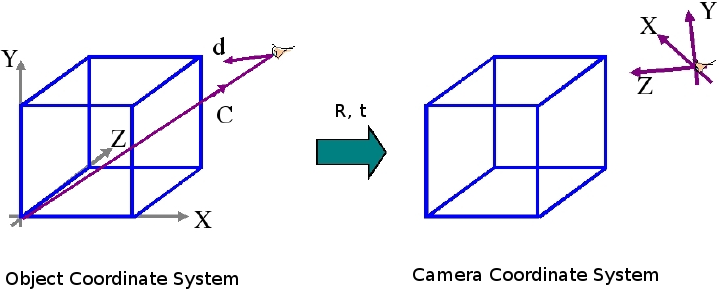
\includegraphics[scale=0.55]{images/camera_object5.png}
\caption{ Mapping points from object coordinates to camera coordinates using
  rotation and translation. The displacement of the origin of the camera system
  from the origin of the object system is $\mathbf{C}$. The camera is viewing in
the direction of the vector $d$. Taken from \cite{graphics}}
\label{fg:objCam}
\end{figure}

The rotation of the object in $n$ dimensions can described using
\textit{Givens rotations} \cite{matrix}. A Givens rotation has the form
\begin{equation}\label{eq:givens}
\mathit{G}(i,k,\theta) = 
\bordermatrix{
&&&i&&k& \cr
&1&\dotso&0&\dotso&0&\dotso&0 \cr
&\vdots&\ddots&\vdots&&\vdots&&\vdots \cr
i&0&\dotso&c_\theta&\dotso&s_\theta&\dotso&0 \cr
&\vdots&&\vdots&\ddots&\vdots&&\vdots \cr
k&0&\dotso&-s_\theta&\dotso&c_\theta&\dotso&0 \cr
&\vdots&&\vdots&&\vdots&\ddots&\vdots \cr
&0&\dotso&0&\dotso&0&\dotso&1 \cr
}
\end{equation}
where $c_\theta = \cos(\theta)$ and $s_\theta = \sin(\theta)$. Pre-multiplying with the Givens
rotation $\mathit{G}(i,k,\theta)^T$ corresponds to a counterclockwise rotation
by $\theta$ radians in the $(i,k)$ coordinate plane, pre-multiplying with
$\mathit{G}(i,k,\theta)$ rotates the the $(i,k)$ plane by $\theta$ radians in
clockwise direction.

From the Pythagorean theorem $\cos(\theta)^2 + \sin(\theta)^2 = 1$ and the symmetries of the sine and cosine function $\cos(-\theta) =
\cos(\theta)$, $\sin(-\theta) = -\sin(\theta)$, it is obvious that Givens rotations are
orthogonal.
\begin{equation}
\mathit{G}(i,k,\theta)^T\mathit{G}(i,k,\theta) =
\mathit{G}(i,k,\theta)\mathit{G}(i,k,\theta)^T = \mathbf{I}
\end{equation}
The transposed Givens rotation amounts to a rotation in the opposite direction by
the same angle thus the two rotations cancel out.

To describe the rotation of the object in three dimensional space we
use the following Givens rotations
\begin{align}\label{eq:rotations}
R_x(\phi) &= \begin{pmatrix}1&0&0\\0&c_\phi&s_\phi\\0&-s_\phi&c_\phi\end{pmatrix} &  R_y(\psi)
  &= \begin{pmatrix}c_\psi&0&-s_\psi\\0&1&0\\s_\psi&0&c_\psi\end{pmatrix}
 & R_z(\theta) &= \begin{pmatrix}c_\theta&s_\theta&0\\-s_\theta&c_\theta&0\\0&0&1\end{pmatrix}
\end{align}
Note that the matrix $R_y(\psi)$ is in fact the transposed Givens rotation. This
is due to the fact that we are interested in describing a left handed coordinate\footnotemark \footnotetext{Some authors
  prefer to instead use the right handed coordinate system to describe an arbitrary 3D
  rotation.} system with the positive $X$ axis pointing up, the positive $Y$
axis pointing to the right and the $Z$ axis pointing into the page. As such the
rotation around the $(X,Z)$ plane needs to be described by the 
Given a point $\mathbf{x} = (x,y,z)^T$ the pre-multiplication with the
Givens rotation $R_z(\theta)$ produces a new point $\mathbf{x'} = (x',y',z')^T$ such that 
\begin{equation}\label{eq:rotated}
R_z(\theta) \mathbf{x} = \begin{pmatrix}c_\theta&s_\theta&0\\-s_\theta&c_\theta&0\\0&0&1\end{pmatrix}\begin{pmatrix}x\\y\\z\end{pmatrix}
    = \begin{pmatrix}c_\theta x + s_\theta y\\c_\theta y - s_\theta
      x\\z\end{pmatrix} = \begin{pmatrix}x'\\y'\\z'\end{pmatrix} = \mathbf{x'}
\end{equation}
The expressions for the $x'$ and $y'$ component of the new point correspond to a
rotation of the $(X,Y)$ coordinate system by $\theta$ radians about the $Z$
axis. These expressions are computed using simple trigonometrics where the point
is decomposed into its $x$ and $y$ components which are then projected on the rotated
$(X',Y')$ axes as can be seen in figure \ref{fg:rotations}. 

\begin{figure}[H] 
\centering
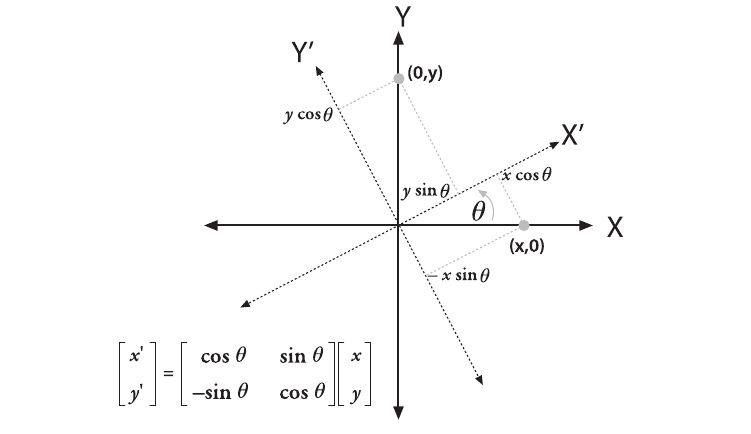
\includegraphics[scale=0.75]{images/rotation.png}
\caption{Transforming one point into another by rotating the coordinate system
  counterclockwise by $\theta$ radians. The point $[x,y]^T$ can be written as $[x,0]^T+[0,y]^T.$ These components
are then individually transformed by projecting them onto the axes of the new
coordinate system $(X',Y')$ to obtain the new point $[x',y']^T$. The new point
is the result of turning the original point clockwise by $\theta$ radians.}
\label{fg:rotations}
\end{figure}

After the transformation in equation \ref{eq:rotated} the $z$ component of the original point is left
unchanged. From similar calculations it can be seen that with matrix $R_y$ the $y$ component, with $R_z$ the $z$ component
remain unchanged. It is therefore apparent that the matrix $R_x(\phi)$ rotates by $\phi$ about the $X$ axis, matrix $R_y(\psi)$ rotates
by $\psi$ about the $Y$ axis and $R_z(\theta)$ rotates by $\theta$ about the $Z$
axis. Any arbitrary rotation in 3D space can then be
achieved using the total \textit{rotation matrix} $R = R_x(\phi)R_y(\psi)R_z(\theta)$ with the
appropriate angles. Since all the total rotation matrix is a product of three
orthogonal Givens rotations it likewise orthogonal with $R^T R = RR^T =
\mathbf{I}$, with $\mathbf{I}$ being the identity matrix. The three angles $\theta$, $\phi$ and $\psi$ represent the three
rotational degrees of freedom (DOF) of the object.

Any position in three dimensional space can be achieved through a
linear combination of movements in any of the three unit directions given by the $X$, $Y$
and $Z$ axes. The \textit{translation vector} allows us to represent the shift
from one coordinate system to another. In terms of the camera coordinate system
and the object coordinate system, the translation vector is the offset between
the origin of the camera system and the object system. Thus, to represent the
position of the object we use the translation vector $t = origin_{object} -
origin_{camera}$. The displacements in the the the unit directions $(1,0,0)^T$,
$(0,1,0)^T$, $(0,0,1)^T$ are given by the components vector $t =
(t_x,t_y,t_z)^T$. 

Equation \ref{eq:rottran} shows how the rotation matrix and the translation vector allow us to transform a point $P
= (p_x,p_y,p_z)^T$
from the object coordinate system to the camera coordinate system. 

\begin{equation}\label{eq:rottran}
\begin{pmatrix}x\\y\\z\end{pmatrix} =
  R\begin{pmatrix}p_x\\p_y\\p_z\end{pmatrix} + t
\end{equation}

With homogeneous coordinates the 6 degrees of freedom (also known as the
extrinsic parameters) can be used to
construct a joint rotation-translation matrix which transforms the 3D point
$Q = (p_x,p_y,p_z,1)^T$ in the object coordinate system to a point $\mathbf{x}
= (x,y,z,s)^T$ in the camera coordinate system as
\begin{equation}\label{eq:jointrottran}
\begin{pmatrix}x\\y\\z\\s\end{pmatrix} =
  \begin{pmatrix}R&t\\\mathbf{0}&1\end{pmatrix}\begin{pmatrix}p_x\\p_y\\p_z\\1\end{pmatrix}
\end{equation}
where $\mathbf{0} = (0,0,0)$. 


\subsection{Pose estimation with the POSIT algorithm !NEW}\label{posit}
Davis and DeMenthon's POSIT algorithm \cite{POSIT}, \cite{opencv} is a simple and efficient method for solving the PnP
problem. The POSIT algorithm estimates the rotation matrix $R$ and the
translation vector $t$
of an object, given a perspective camera with known parameters, at least 4 non-coplanar feature points on the 3D object and the corresponding
projections of these points in the 2D image. To compute an approximation of the
true $R$ and $t$, we first expresses the camera coordinate system in terms of
the object coordinate system. Since the rotation matrix aligns the axes of the
two coordinate systems we therefore know that the rows $i$, $j$ and $k$ of the
rotation matrix correspond to the unit vectors of the camera coordinate
system expressed in the object coordinate system. 

This is easy when on the
example of the camera system unit vector $u = (1,0,0)^T$. The rotation matrix
$R$ transforms a vector $x$ from the object coordinate system into $u$,
therefore $u = Rx$. The rotation matrix is orthogonal so if we turn in the
opposite direction we get $x = R^Tu$ as the object system equivalent of $u$. Since $u = (1,0,0)^T$ we obtain the first
row of the rotation matrix $R$ as the object coordinate system vector which
corresponds to $u$.

The rotation matrix can therefore be written as
\begin{equation}
R = \begin{pmatrix}i_1&i_2&i_3\\j_1&j_2&j_3\\k_1&k_2&k_3\end{pmatrix}
\end{equation}
Since the three vectors $i$, $j$ and $k$ are all orthogonal we only need to find the
first two and obtain the third as the cross product of the other two.

The translation vector is specified as the vector $\overrightarrow{OM_0}$ between the
origin of the camera system $O$ and the origin of the object system $M_0$. The
point $M_0$ can be conveniently picked as one off the known feature
points. Unfortunately, the
camera coordinate system equivalent of this point is unknown since we do not
know the rotation matrix. However, the translation vector can be expressed in
terms of the 2D projection of this feature point
as $t = \frac{Z_0}{f}\overrightarrow{Om_0}$ where $m_0$ is the known 2D projection of $M_0$
and $Z_0$ is the $z$-component of the translation vector. Therefore, to estimate
the 3D pose we need to find the values of $i$, $j$ and $Z_0$.

The POSIT algorithm first makes a rough estimate these values using a \textit{pose from
  orthography and scaling} (POS) step. In the POS step it is assumed that the
points are far enough from the camera so that we can assume a weak-perspective
camera model. Using this camera model the values $i$, $j$ and $Z_0$ all have
closed form solutions. After this first step, the 2D image are then projected back into the object
coordinate space with using the true perspective camera and the pose (rotation,
translation) estimated in the POS step. These new points are then used in further
in POS steps until the algorithm converges, hence the name POS with iterations
(POSIT). However, it is important to note that the convergence of the algorithm
depends heavily on the weak-perspective assumption that the internal depth of
the object is small compared to the distance from the pinhole camera.

The fundamental equations of the POSIT algorithm are
\begin{gather}\label{eq:posit}
\overrightarrow{M_0M_i}\cdot I  = x_i(1+\varepsilon_i) - x_0\\
\label{eq:posit2}
\overrightarrow{M_0M_i}\cdot J  = y_i(1+\varepsilon_i) - y_0
\end{gather}
with
\begin{equation*}
I = \frac{f}{Z_0}i \mathrm{, }\quad J = \frac{f}{Z_0}j \quad \mathrm{and} \quad
\varepsilon_i = \frac{1}{Z_0}\overrightarrow{M_0M_i} \cdot k
\end{equation*}
During the POSIT iterations, values are given to $\varepsilon_i$ starting with
0 in the first iteration and then computed from $\varepsilon_i =
\frac{1}{Z_0}\overrightarrow{M_0M_i} \cdot k$ with the $k$ and $Z_0$ being guesses from the
previous iteration. Then the system of equations given by \ref{eq:posit},
\ref{eq:posit2} is solved to obtain the vectors $I$ and $J$. These vectors are
normalized to get the two rows of the rotation matrix $i$ and $j$. The
$z$-component of the translation vector $Z_0$ is given by the norm of either $I$
or $J$.

\section{Feature Point Tracking}
As we have seen, most model based recognition techniques rely on a number identified feature
(landmark) points to estimate the model parameters. To be able to track a model
between successive frames of a video recording, it is therefore necessary to
either keep locating the points in every frame or to track the movement points
themselves. This problem of tracking the movement points or objects between
images has spurred the development of many algorithms. Most of these algorithms
fall into the \textit{optical flow} category since they determine the movement
of points based on the intensity changes at pixels. One such algorithm is the
Kanade-Lucas-Tomasi feature tracker.
\subsection{Kanade-Lucas-Tomasi Feature Tracker}\label{s:kanade}
Kanade and Lucas first introduced an iterative feature point registration algorithm in
\cite{kanade}. Tomasi and Kanade developed a more generalized version of
algorithm in \cite{kanade2}, \cite{kanade3}. The derivation of the algorithm is
given by Birchfield in \cite{kanade4}.

The problem of registering a displaced image can between two images is
formalized by assuming there are two images functions $F(\mathbf{x})$ and $G(\mathbf{x})$. The image
functions take a vector $\mathbf{x} = (x,y)^T$ as input
and output the pixel intensity at $\mathbf{x}$. The goal in image registration
is to find a disparity vector $\mathbf{h} = (h_x,h_y)^T$ which minimizes
a measure of difference between $F(\mathbf{x + h})$ and $G(\mathbf{x})$ for a given window of
interest $\mathcal{W}$. The windows is required, since it is very difficult to
track single pixels as they can be easily confused with other pixels unless they
have very distinct brightness. The window of interest contains a number of
pixels and should contain sufficient texture. The feature tracking is
illustrated in figure \ref{fg:apple} where the apple is the window of interest.

\begin{figure}[H] 
\centering
\setlength\fboxsep{0.5pt}
\setlength\fboxrule{0.5pt}
\label{fg:apple}
\subfloat[F(x)]{
  \fbox{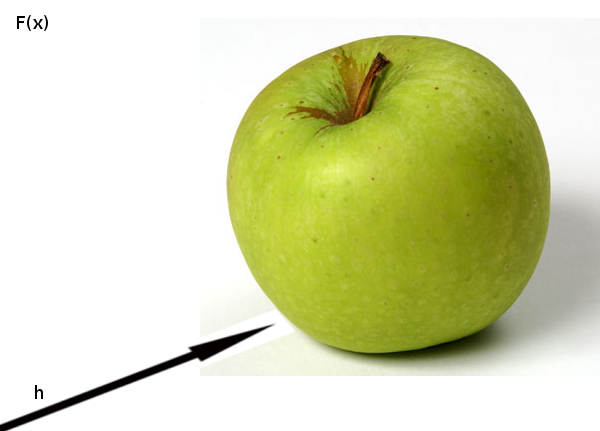
\includegraphics[scale=0.35]{images/fx.png}}
}
\subfloat[G(x)]{
  \fbox{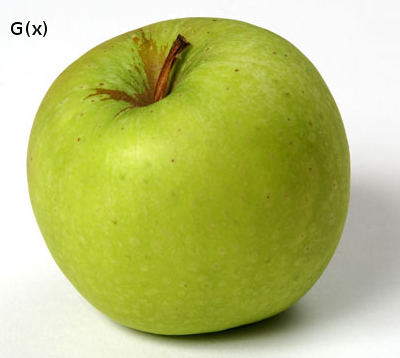
\includegraphics[scale=0.35]{images/gx.png}}
}
\caption{ The image registration problem. The task is to find the disparity
  vector $h$.}
\end{figure}

The optimal displacement vector $\mathbf{h}$ minimizes the error function $E$ which is
given by
\begin{equation}
E(\mathbf{h}) = \int_{\mathcal{W}} (F(x + h) - G(x))^2 \mathop{d}x
\end{equation}

The naive way to locate this $h$  would be to iterate through all the possible values of $h$ and measure the $E(\mathbf{h})$ norm. A
better approach was proposed by Kanade and Lucas. The behavior
of the function $F(\mathbf{x})$ is approximated using a first order Taylor expansion as 
\begin{equation}\label{eq:kanade1}
F(\mathbf{x + h}) \approx F(\mathbf{x}) + \mathbf{g}^T\mathbf{h}
\end{equation}
where 
\begin{equation}
\mathbf{g} = \bigr[ \begin{smallmatrix} \frac{\partial}{\partial x}
    \bigr(\frac{F + G}{2}\bigl) \quad \frac{\partial}{\partial y} \bigr(\frac{F + G}{2}\bigl) \end{smallmatrix} \bigl]^T
\end{equation} 
This approximation is used instead of $F(\mathbf{x + h})$ in the error. Then the minimum of the error
function is located by setting the derivative of the error function with respect
to $\mathbf{h}$ to zero. Therefore
\begin{align}\label{eq:kanade2}
\frac{\partial E}{\partial \mathbf{h}} = \frac{\partial}{\partial \mathbf{h}}
\int_{\mathcal{W}} (F(x) + \mathbf{g}^T\mathbf{h} - G(x))^2 \mathrm{d}x =
2\int_{\mathcal{W}} \mathrm{g}(F(x) + \mathbf{g}^T\mathbf{h} - G(x))
\mathrm{d}x
\end{align}
Setting the above to zero and rearranging the terms we get the fundamental
equation which relates the spatial intensity to the optimal displacement
$\mathbf{h}$ as
\begin{align}\label{eq:kanade3}
\Bigr(\int_{\mathcal{W}} \mathbf{g}\mathbf{g}^T\mathrm{d}x\Bigl)\mathbf{h} = \int_{\mathcal{W}} \mathrm{g}(F(x) - G(x))
\mathrm{d}x
\end{align}
In matrix form the equation \ref{eq:kanade3} can be expressed as
\begin{equation}\label{eq:kanade4}
\mathbf{Z}\mathbf{h} = \mathbf{e}
\end{equation}
The iterative Kanade-Lucas algorithm specifies the order in which possible values of $\mathbf{h}$ will be explored. The procedure
iteratively improves the guess for $\mathbf{h}$ by solving the equation
\ref{eq:kanade3} with the spatial intensity
gradients evaluated at each point $\mathbf{x}$ in the image. Thus, the algorithm locally searches for the best disparity vector $\mathbf{h}$ by using the
information about the gradient at all points in the image. The estimation of the
$\mathbf{h}$ and the convergence of the algorithm is further improved by
weighing contributions of the points $\mathbf{x}$ inside the window. The
weighing function can be a Gaussian or just set as $w(\mathbf{x}) = 1$.

The integrals simplify to sums when we are dealing with pixel values in real images.
The iterative scheme for the Kanade-Lucas-Tomasi feature tracking algorithm is therefore:
\begin{align}
& \mathbf{h}_0 = 0\\
& \mathbf{h}_{k+1} = \mathbf{h}_k + \frac{\sum_{ \mathbf{x} \in \mathcal{W}} w(\mathbf{x}) \mathbf{g}[G(x) - F(\mathbf{x} + \mathbf{h}_k)]}{\sum_{ \mathbf{x} \in \mathcal{W}} w(\mathbf{x}) \mathbf{g}\mathbf{g}^T}
\end{align}

To further improve the technique it can be performed with several resolution levels, using the result from the coarser resolution as starting
$h_0$ of the algorithm with a finer resolution. An effective variation of the
algorithm which utilizes this approach was developed by Bouguet
\cite{kanade4}. Bouguet's implementation of the Kanade-Lucas-Tomasi algorithm
uses several resolution levels from highest to lowest. These resolutions
resemble a pyramid of images, which is why this implementation is called the
pyramid Lucas-Kanade tracker. At every level of the pyramid the iterations are
computed to and the guess is propagated to the lower of the pyramid.

The algorithm can also successfully compute the $h$ even if the region of interest has been rotated or
scaled. If the image has been rotated or scaled we express the matching problem
as $G(x) = F(xA +h)$ where $A$ is a linear transformation matrix. This
transformation allows us
to apply the algorithm.

The Kanade-Lucas-Tomasi feature tracker has been successfully applied to
tracking facial feature points \cite{faceTransfer05}. Vlasic et al localized
feature points in the initial frame manually and then used the
Kanade-Lucas-Tomasi feature tracker to obtain the displacements between pairs of
frames. From these displacements they were able to derive parameters for their
tensor-based multilinear model. This allowed them to transfer expressions to
another video performance.

As a local iterative search method, the Kanade-Lucas-Tomasi feature tracker's
performance depends heavily on the initial guess of the $h$. If the initial
guess is too far from the region of interest then the algorithm does not perform
well, since the scheme was derived using local approximations of
functions. These local approximations will not hold for points far from the
region of interest.


\section{Optimization}
The task of locating the correct model parameters which match the model to an
object in the image is an optimization problem. It may not be possible to find
an exact match which would explain the object in the image perfectly. Therefore,
we are interested in finding an instance of the model which is most similar to the
object in the image. One way to measure dissimilarity is through the use of an error function. If the
value of the error function is large it means that the two entities are
dissimilar. To find a model instance which is most similar we therefore need to
minimize the error function. Optimization techniques make it possible to locate
minima of functions.

\subsection{Least Squares and Non Negative Least Squares}
An important error function, which is often utilized in statistics and engineering, is the
sum of squares error. This error function defines the dissimilarity between input
values $y_i$ and target values $t_i$ using a numeric value given by
\begin{equation}\label{eq:nnls}
E(y) = \sum_i (y_i - t_i)^2
\end{equation}
Solving a problem in the least squares sense means minimizing this error
function. Given is a linear system of equations defined in matrix notation by
$\mathbf{A}\mathbf{x} = \mathbf{b}$ with $\mathbf{A} \in \mathbb{R}^{m\times
  n}$, $\mathbf{x} \in \mathbb{R}^{n\times 1}$ and $\mathbf{b} \in
\mathbb{R}^{m\times 1}$. This linear system may not have an exact solution if it
is over determined $m > n$, underdetermined $m < n$  or more generally when
$\mathbf{A}$ is not invertible. Solving this linear system in the least squares sense
means finding a $\mathbf{\hat{x}}$ for which the following error function is
minimized
\begin{equation}\label{eq:nnls2}
E(\mathbf{\hat{x}}) = \frac{1}{2}\lVert \mathbf{b} - \mathbf{A\hat{x}} \rVert^2
\end{equation}
with $\lVert . \rVert$ being the vector norm (distance).
To find this minimum we take the derivation of \ref{eq:nnls2} with respect to
$\mathbf{\hat{x}}$ and set it to zero. The least squares solution is therefore
\begin{equation}\label{eq:nnls2}
\mathbf{\hat{x}} = (\mathbf{A}^T\mathbf{A})^{-1}\mathbf{A}^T\mathbf{b}
\end{equation}
where the expression $(\mathbf{A}^T\mathbf{A})^{-1}\mathbf{A}^T$ is commonly
known as the pseudo-inverse.

It is also possible to find the least squares solution of a linear system using
singular value decomposition \cite{Press1992} if the matrix $\mathbf{A}$ is square. Usually the linear system would
be solved by inverting $\mathbf{A}$ and pre-multiplying the equation with this
inverse. Given the SVD $\mathbf{A} = \mathbf{U\Sigma V}^T$ we can easily invert
$\mathbf{A}$ by inverting the right hand side to get $\mathbf{A}^{-1} =
\mathbf{V\Sigma}^{-1}\mathbf{U}^T$. If the square $\mathbf{A}$ is not invertible it
means that some of the diagonal elements in $\Sigma$ are 0. However, We obtain a
least squares solution by inverting the non-zero elements of $\Sigma$ and
pre-multiplying with $\mathbf{V\Sigma}^{-1}\mathbf{U}^T$.

In some case it may be necessary to enforce constraints on the function. This is
particularly important when the variables represent real physical entities,
which should not be negative. Such non negativity constraints are often
introduced to a linear system. The goal of optimization is then to solve this
non negativity linear system in the least squares sense. The problem is
therefore to find the $\mathbf{x^*}$ for which holds
\begin{equation}\label{eq:nnls3}
\mathbf{x^*} = \underset{\mathbf{x} \ge 0}{\mathrm{argmin}} \frac{1}{2}\lVert \mathbf{b} - \mathbf{Ax} \rVert^2
\end{equation}
To optimize this constrained error function Franc et al reformulate the problem as an equivalent
quadratic optimization problem \cite{nnls}, \cite{nnls2}. 
\begin{equation}\label{eq:nnls4}
\mathbf{x^*} =  \underset{\mathbf{x} \ge 0}{\mathrm{argmin}} \Bigr( \frac{1}{2}
\mathbf{x}^T\mathbf{H}\mathbf{x} + \mathbf{x}^T\mathbf{f} \Bigl)
\end{equation}
where $\mathbf{H} = \mathbf{A}^T\mathbf{A}$ and $\mathbf{f} = -\mathbf{A}^T\mathbf{b}$.
Franc et al solve this quadratic optimization problem by first formulating the Karush-Kuhn-Tucker (KKT) conditions
and then applying a sequential coordinate descent algorithm. The KKT conditions for the non negative least squares solution are
given by
\begin{align}\label{eq:nnls5}
\mathbf{H}\mathbf{x} + \mathbf{f} - \mathbf{\mu} &= \mathbf{0}\\
\mathbf{x} &\ge \mathbf{0}\\
\mathbf{\mu} &\ge \mathbf{0}\\
\mathbf{x}^T\mathbf{\mu} &= 0
\end{align}
The sequential coordinate-wise algorithm (SCA) then computes this solution so that the
KKT conditions are satisfied. The SCA non-negativity least squares algorithm is
given in \ref{a:sca}. The input matrices are  $\mathbf{H} =
\mathbf{A}^T\mathbf{A}$, $\mathbf{f} = -\mathbf{A}^T\mathbf{b}$ and
$\mathbf{h}_k$ denotes a column of the matrix $\mathbf{H}$. 

\begin{algorithm}\label{a:sca}
\caption{Sequential Coordinate-wise Non-negativity Least Squares Algorithm}
\begin{algorithmic}[1]
\Procedure{SCANNLS}{$\mathbf{H}$,$\mathbf{f}$}
\State \textbf{Output} $\mathbf{x^*} \ge 0$ such that $\mathbf{x^*} =
\mathrm{argmin} \frac{1}{2}\lVert \mathbf{Ax - b} \rVert^2$
\State \textbf{Initialization} $\mathbf{x}^0 = \mathbf{0}$ and $\mathbf{\mu}^0 =
\mathbf{f}$
\State \textbf{repeat}
\For {$k = 1 \ldots n$}

\State $\mathbf{x}_k^{t+1} = \mathrm{max} \Bigr(0,\mathbf{x}_k^t -
\frac{\mathbf{\mu}_k^t}{\mathbf{H}_{k,k}} \Bigl)$
\State $ \mathbf{x}_i^{t+1} = \mathbf{x}_i^{t+1} \quad \forall i \ne k$

\State $\mathbf{\mu}^{t+1} = \mathbf{\mu}^t + (\mathbf{x}_k^{t+1} - \mathbf{x}_k^t)\mathbf{h}_k$

\EndFor

\State \textbf{until} stopping criteria (KKT conditions) are met.
\EndProcedure
\end{algorithmic}
\end{algorithm}



\subsection{Nelder Mead Downhill Simplex}\label{s:nelder}

The downhill simplex is a local optimization method that does not
require gradients to identify local extrema. With the downhill simplex method a
local optimum is found by means of a sequence of fitness function evaluations.

The downhill simplex method was coined by Nelder and Mead in 1965
and has since proven itself to be comparable in efficiency to the more popular 
gradient based optimization methods. The method was designed
for the optimization of multidimensional, unconstrained functions
that have either no gradients or when the gradient exist only for
portions of the search space such as in the case of discontinuous functions
\cite{Nelder2009}. However, the drawback of the method is that many fitness function evaluations
are required. Therefore, when the computational complexity of the
fitness function is very high, other optimization methods need to
be considered instead of the Nelder Mead downhill simplex \cite{Press1992}.

The algorithm is based on the idea of isolating the
minimum by geometrically transforming a \textit{simplex}. The simplex
is a convex hull of $N+1$ vertices, where $N$ is the underlying
problem's dimension. In a two dimensional space this simplex would therefore
be a triangle, in three dimensions a tetrahedron. The algorithm is initialized
so that the simplex encloses
a portion of the search space and the goal is to move the simplex along the
search space surface and deform so that all of its vertices converge on the local optimum. This is achieved with
the help of geometric transformations of the simplex.

The process of transforming a multidimensional simplex, in order to
isolate the minimum, is somewhat analogous to bracketing a minimum
in a one dimensional search space. The one dimensional search space will have
peaks and valleys in places of local optima. The simplex, which is a line in one
dimensional space, makes it's way downhill
through this search space, in search of a minimum by means of shrinking and
stretching. When the simplex finds a local minimum, it shrinks itself to contain
only the minimum and the algorithm terminates.

The behavior of the simplex during the algorithm parallels the expanding and
collapsing movements of the amoeba
organism. The Nelder Mead downhill simplex is in
some publications referred to as the \textit{amoeba} method due to this similarity but also to distinguish it from Dantzig's
simplex method for linear programming \cite{Press1992}. 


\subsubsection{The Downhill Simplex Algorithm}

To initialize the downhill simplex algorithm we need a nonlinear fitness function $f\,:\,\mathbb{R}^{N}\rightarrow\mathbb{R}$
and an initial point $P_{0}$. The simplex will be a $N+1$ dimensional convex
hull. The first vertex of the convex hull is the initial point. The remaining
$N$ vertices $P_{i}$ are derived from the initial point. The shape of the simplex defines the way in which the
points $P_{i}$ are calculated\cite{Nelder2009}.

The simplex shape can be one of the following:
\begin{itemize}
\item The simplex can have a regular shape where all sides are equally
long. It is up to the user to pick this length.
\item The simplex can be right angled in which case the vertices
$P_{i}$ are calculated according to formula \ref{eq:right_angle_simplex}.


\begin{equation}\label{eq:right_angle_simplex}
P_{i}=P_{0}+\lambda e_{i}
\end{equation}
\\
where $e_{i}$ are unit vectors for the $N$ dimensions and $\lambda$
is a constant. This constant influences the size of the simplex and
represents a guess of the problem's characteristic scale length \cite{Press1992}.
\end{itemize}

After the initialization phase, three crucial steps are repeated
until the simplex has encountered the local minimum. These steps are
based around moving the vertex of the simplex with the largest fitness
function largest value to a new point where the value will be
smaller. 

\begin{enumerate}
\item[\textbf{1.}] The first step is to sort the vertices
$x_{i}$ of the simplex from worst to best, where $h$ is the index
of the worst vertex, $s$ the second worst index and $l$ the best
index.
\item[\textbf{2.}] Then the \textit{centroid} of the best side is calculated according
to formula \ref{eq:centroid}.\\
\begin{equation}\label{eq:centroid}
c=\frac{1}{N}\sum_{j\neq h}x_{j}\end{equation}
\\
\item[\textbf{3.}] In the final step, the centroid is used to geometrically
  transform the simplex in order to move the current worst vertex to
a better position. To achieve this, the algorithm seeks a replacement point for $x_{h}$
on the line that connects the worst index $x_{h}$ and the centroid
$c$. Three different points are then compared and the one with the best fitness
value is chosen as the replacement point. These three candidates are obtained
using reflection (formula \ref{eq:reflection}), expansion (formula
\ref{eq:expansion}) and either inside or outside contraction (formula \ref{eq:contraction}). \\
\begin{equation}\label{eq:reflection}
x_{r}=c+\alpha(c-x_{h})
\end{equation}

\begin{equation}\label{eq:expansion}
x_{e}=c+\gamma(x_{r}-c)
\end{equation}

\begin{equation}\label{eq:contraction}
x_{c}=\begin{cases}
c+\beta(x_{r}-c) & if\, x_{h}\leq x_{r}\\
c+\beta(x_{h}-c) & else\end{cases}
\end{equation}

In case neither of these three new replacement point candidates has
a better fitness value than the worst vertex $x_{h}$, then the entire
simplex is shrunk towards the best vertex $x_{l}$. In this case $N$
new vertices will be computed as follows:\\
\begin{equation}
x_{j}=x_{l}+\delta(x_{j}-x_{l})\,\,\,\, j=0,\ldots,N\,\wedge\, j\neq l\end{equation}
\\
The geometric implications of the transformations reflection, expansion,
contraction and shrinking are depicted in figure \ref{fg:amoeba}. 

\end{enumerate}


%
\begin{figure}[H]
\begin{centering}
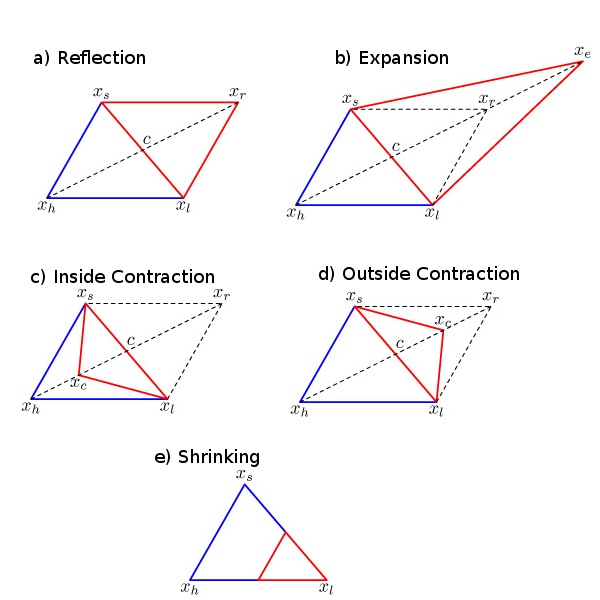
\includegraphics[scale=0.55]{images/amoeba}
\par\end{centering}

\caption{Geometric interpretations of the simplex transformations. Taken from
\cite{Nelder2009}}
\label{fg:amoeba}

\end{figure}


The transformations are controlled by four parameters $\alpha$ for
reflection, $\beta$ for contraction, $\gamma$ for expansion and
$\delta$ for shrinking. Most implementations use the standard values
$\alpha=1$, $\beta=\frac{1}{2}$, $\gamma=2$ and a shrinking by
a half with $\delta=\frac{1}{2}$ \cite{Press1992,Nelder2009}. 

Finally, since the algorithm should terminate in finite time, it is
necessary to establish a termination criterion. If the execution of
the three aforementioned steps is considered one cycle of the algorithm,
then possible termination criteria include terminating when the vector
distance moved in the cycle was smaller than a constant tolerance
$tol$, or when the difference between the fitness value of the newly
obtained best and the old best is no larger than a tolerance $ftol$.
Since either of these criteria could occur in a single anomalous step,
restarts of the downhill algorithm are also sometimes utilized \cite{Press1992}. 


\chapter{Design}\label{design}
In this chapter we will design an application which understands the facial
dynamics captured in a video recording of an individual. This understanding is
accomplished by correctly modeling the shape of this individual's face.

The goal of the application is to transfer the expressions between two
subjects. Given are video recordings of two persons and a database of
faces. One recording is the source of the expressions, henceforth just source. The
other recording is the target. The task is to alter the target recording so that
the target person's face is animated to perform the expressions seen in the
source.

We approach this problem by constructing a deformable shape model of a face from the
face database. The model is constructed so that every expression corresponds to a specific instance of the model
parameters. Since the goal is to transfer expressions, the model should be able
to alter expression and identity of the subject separately. This suggests that the optimal model should have
separate parameters for these two attributes, to allow the user to manipulate
the identity independently of the expression or vice versa.
As discussed in
section \ref{works}, the tensor-based model possesses this very
important quality of separability which makes it suitable to use as the
deformable model of choice in the expression transfer application.

To find the values of the parameters, the model is fitted frame-by-frame to the source recording using an
algorithm that estimates the 3D pose of the model, the expression parameters and
the identity parameters. The model is also fitted to the target recording to obtain a model of the target face. The
parameters from the source model are then used to animate the target model.

The application therefore needs to be designed to support the following functionality:

\begin{enumerate}
\item Pre-processing of the face database.
\item Learning a tensor-based model from the face scans in pre-processed database.
\item Implementation of an algorithm to find the expression, identity and pose
  parameters of the face in the source and target recording.
\item Animating the target face with the expression parameters estimated from
  the source face.
\end{enumerate}

To make the application user-friendly, the implementation of this functionality should be encapsulated in
graphical user interface (GUI). This GUI needs to be built with support for a 3D
rendering framework since the application has to display the three-dimensional models and animate
the target face. Additionally, most of the tasks that the application needs to
solve either involve linear algebra computations or can be solved with standard
computer vision algorithms. The implementations of these computations and
algorithms need to be as efficient as possible to ensure that the application is
highly responsive to the users actions and commands.

\section{Design Challenges}
While it may seem like a trivial problem to a human, the task of transferring expressions involves many
challenges. The computer is attempting to understand a face using its model of
what a face should look like, as well as recognize the face in images and follow
its movements through successive frames. All the while, the application has to 
correctly interpret all the observed deformations as corresponding expressions.  

The first challenge lies in developing an algorithm that fits a model to a face in
the image. Two expressions can differ in only very little detail and yet this
small amount of detail can make a huge difference to how a human observer
interprets the expression. A slight difference in the position of the corner of
the mouth is all that separates a smirk from a genuine smile. However, model based
recognition revolves around approximating an object in the image with an
instance of the model. So if it is to correctly identify expression, the
algorithm needs to operate on a large
number of points to minimize the error between the approximation and the
observed face as much as possible. This first of all causes the algorithm to take
more time, but it also directly leads to the second problem of how these points
are to be chosen. 

The model fitting is performed with an error minimization algorithm. To perform
this minimization, reference measurements are needed against which the minimization is
performed. These measurements will be points in the frames which comprise the
video sequences. These points should of course be points located on the
face. So before the algorithm can begin fitting a model, it first needs some
information about where the face is located in the image. However, it is not
only necessary to identify the general position of the face -- it is in fact
imperative to know the position of points on the face which correspond to points in the
model. Depending on how the face is located it may prove to be difficult to
obtain more points to use in the fitting.

A convenient approach is to locate the face in only the first frame of the video
sequence. Its position in the successive frames is then obtained by tracking the
movement of the face from the first frame. Therefore, before applying the
fitting algorithm the application needs to perform the following two steps:
\begin{enumerate}
\item Locating feature points in the first frame of both the source and target
  recording.
\item Tracking the movement of the feature points to obtain a guess for feature
  points in every frame.
\end{enumerate}

Yet this tracking is again an approximation. It often also happens that certain points in the face are lost
during the tracking procedure. So again it is impossible to guarantee that the
fitting algorithm will be able to recover sufficient level of detail to correctly estimate the expression.


The final and most crucial problem lies in the fact that usually only very specific
areas of the face contribute to expressions. The mouth or the brow are excellent
areas for reference points for the fitting algorithm. However, should points in these
areas be lost during tracking, or misidentified during face location then it is
very likely that an incorrect expression will be estimated. Even if only a small
number of points is lost, the algorithm can still fail badly if these were
points from an important part of the face.

It is clear that error accumulates in every step of the model
fitting. A robust application must therefore attempt to enforce constraints to limit this
accumulation. The fitting algorithm and the model therefore need to be designed
with these considerations in mind.

\section{Frameworks and APIs}
An important design and implementation question when constructing a large
application, is deciding which software application programming interfaces
(APIs) and software frameworks the application should employ. The
great advantages of utilizing APIs and frameworks is that they provide efficient
implementions of algorithms. The disadvantage is that some frameworks may
require the user to install this framework on his machine to be able to use the
application. Quite important is also the quality of cross-platform
compatibility. To desing a portable application only cross-platform
frameworks and APIs should be chosen.

\subsection{OpenCV}
The expression transfer application processes images and utilizes many computer
vision algorithms. An excellent library of computer vision algorithms and
functions is the OpenCV library. The OpenCV is a multi-platform library
written for C and C++ \cite{opencv}. It was designed to provide a simple-to-use
computer vision infrastructure for building vision applications. A large part
of OpenCV was developed by Intel, specifically Intel's Russian branch. The
expression application is build with OpenCV version 2.1.0.

Among the algorithms included in the OpenCV library are efficient implementations the Kanade-Lucas feature tracker
and the POSIT algorithm for 3D pose estimation. The OpenCV library also provides
an excellent matrix data structure.

\subsection{OpenGL}
Since the expression transfer
application deals with a 3D model of the human face, it should be possible for
this model to be presented graphically to the user. To
this end we can use the popular graphics interface OpenGL. The Open Graphics Library (OpenGL) is a software interface to the graphics
hardware \cite{opengl}. It is currently being further developed and maintained
by the Khronos Group. The OpenGL API provides a large
number of commands to render 3D objects. These objects are constructed
from graphics primitives like points, lines and polygons. The rendering of
objects in OpenGL is
implemented using a series of processing stages called the rendering
pipeline. The pipeline also provides numerous useful graphics operations such transformations
between camera and object coordinate systems, texture mapping and lighting. \begin{comment}The
OpenGL code is streamlined, hardware-independent and highly portable, which in
addition to its availability has contributed to OpenGL's popularity.\end{comment}
\subsection{Qt}
The OpenGL graphical representation needs to be encapsulated in a user-friendly graphical user
interface (GUI) to allow the user to load and process the video recordings. The GUI
of choice for the expression transfer application is Trolltech's Qt, because it integrates well
with the OpenGL framework. The Qt framework also includes a build system called qmake, which is
likewise cross-platform. The Qt framework was developed by Trolltech in 1991. The
software has since been acquired by Nokia. \begin{comment}The Qt UI frameworks is a
cross-platform application, which simple to use especially when used together
with the QtCreator IDE. This IDE has a built in graphical editor to create user
interfaces. Of special importance to the expression transfer application is the
possibility to easily integrate a Qt GUI with OpenGL. \end{comment} 


\section{Pre-processing}
The primary drawback of the tensor-based model is that it requires the faces in
the database to be in \textit{correspondence}. To put faces in the database into correspondence
so that a tensor model can be constructed, we must perform pre-processing of the
database data.

\subsection{Correspondence}
For the purpose of this application we consider two polygon meshes to be in correspondence
if for any point in one polygon mesh, the point in the other polygon mesh which corresponds to the
same position on the object, has the same index value. So for example if the
point corresponding to the tip of the nose has an index value of $i$ in one
face, then  there will be a point in the other face with perhaps
different $x$, $y$ and $z$ but the same $i$ index which also corresponds to the
tip of the nose. So essentially, the order of the indices must be the same in both
polygon meshes. 

In the case when the two polygon meshes are not in correspondence, then a
optimization algorithm must be applied to deform the mesh to correspond to a
reference mesh. One mesh may have fewer vertices, or the vertices can be have a different
ordering than in the reference mesh. To standardize the meshes the vertices in
one mesh need to be aligned with vertices in the other mesh. 

Correspondence may be computed in two ways. One approach is to use a
registration algorithm which locates the rigid-transformations that transform a misaligned mesh into the reference mesh. A popular algorithm
for 3D registration is the Iterated Closest Point (ICP) algorithm. Rusinkiewicz
and Levoy give a comprehensive overview of efficient implementations of the ICP
algorithm in \cite{ICP}. The other approach involves finding the minimal deformation of
the polygon mesh which transforms it into the reference mesh. An example of this
type of algorithm was described by Sumner and Popovic in \cite{deformTri}
who achieve this by transferring deformation between triangle meshes.

Other irregularities in the polygonal mesh can be present depending on how the
3D face scans in the database were obtained. For example there can be holes or spikes in the
mesh, which need to be removed by interpolating new points to fill the holes or
by Gaussian smoothing the spikes. 

\subsection{Database}
The face database used in the application is the Binghamton expressions database \cite{binghamton}. This database of 3D face scans was developed at the Department of
Computer Science of the State University of New York at Binghamton. The subjects 
in the face database perform seven expressions -- neutral, angry,
disgust, fear, happy, sad and surprise. Every subject carried out each of these
expressions (except for neutral) in four levels of intensity. 

The Binghamton database was constructed with the help of 100 students who participated in the face
scans. Various ethnic groups are represented and the database consists of about
60\% female and 40\% male subjects. There is an unfortunate lack of middle aged to older
 subjects in the database, due to the fact that mostly students were
involved in face scans. For purposes of the face transfer application this is a clear
disadvantage since it makes the model we construct much less powerful.

The advantage of a 3D face database lies in the fact that it allows us to
construct a 3D model. This 3D model will clearly be more powerful then a 2D
model since it has more degrees of freedom. When the task is to transfer
expressions between two recordings of 3D faces it is preferable to have a 3D model
which should in theory be able to duplicate the exact motions and rotations of the recorded
objects. If the face database consisted of only 2D face images then the model
would also have to be two-dimensional.

The face scans were captured using the 3DMD digitizer which utilizes structured light to
calculate the depth. The captured surfaces contained between 20,000 and 35,000
polygons. Example original face scans, along with the captured texture maps are
shown in figure \ref{fg:binghamton} 

\begin{figure}[H]
\begin{centering}
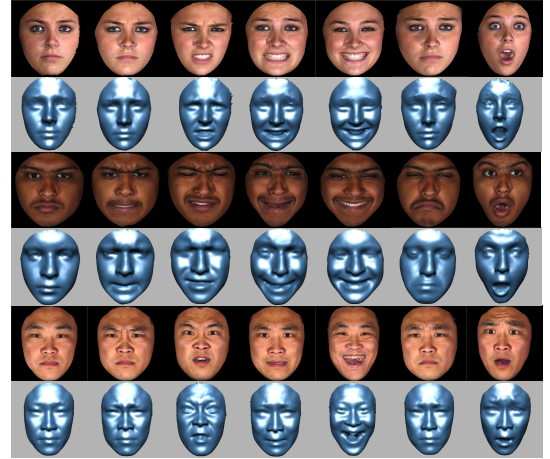
\includegraphics[scale=0.80]{images/binghamton.png}
\par\end{centering}

\caption{Sample 3D face scans from the Binghamton database along with the
  corresponding texture maps. Taken from \cite{binghamton}}
\label{fg:binghamton}

\end{figure}
\clearpage

The Binghamton database consists of faces stored as polygon mesh data in VRML
format and texture information in bitmap format. For the project the pre-processed Binghamton
database was used. This pre-processed database was created by Dr. Lynn-Minoi
\cite{jacey} and consists of VTK files of the pre-processed polygon meshes. The
VTK file lists the $x$, $y$ and $z$ values of every vertex, the topology data
of the face scan and the texture coordinates for every vertex. The face scans in
pre-processed database are in correspondence, meaning that the order of the
vertices in every face scan is the same. Conveniently, having the face scans in
correspondence also means that the topology data stays constant.


The final pre-processing step before building a model is to move the center of the
face scans to the origin of the object coordinate system. This step is not always required. However, the vertices in the
pre-processed Binghamton database have a $z$-component with an average value of
$z_{avg}=-1500$. It serves no purpose to have the face at such a distance. It
can even cause problems to some algorithms like the POSIT algorithm discussed in
\ref{posit}. Moving the center of the face scans to the origin of the object coordinate
system can be done by merely calculating the average $x$, $y$ and $z$ of the
entire dataset and then subtracting this average from every vertex.


\section{Model Construction}
Given a database of 3D face scans that are in correspondence, the tensor-based
model can be constructed by first organizing this data into a tensor and
then using multilinear algebra to find a decomposition of this tensor.

\subsection{Data Tensor}\label{s:datatesnor}
The tensor model should be designed to address expression and identity as sources of variation in
the data. We assume that the points are defined by a set of size $I_{pts}$, the
expressions by a set of size $I_{exp}$ and the identities with size $I_{id}$. Then we can
construct a data tensor $\mathcal{D} \in \mathbb{R}^{I_{pts} \times I_{id}
  \times I_{exp}}$. Each face scan in the database is vector from
$R^{I_{pts}}$ and there are $I_{id}I_{exp}$ such vectors in the database. To load data into the the tensor we need to read each vector
representing a face into the tensor and index the elements of this vector
appropriately. This is done as follows

\begin{algorithm}\label{a:load}
\caption{Loading the Data Tensor}
\begin{algorithmic}[1]
\Procedure{Load}{database,$\mathcal{D}$} \Comment{Input the database and the
  empty data tensor}
\For {$i = 1 \ldots I_{id}$}
\For {$j = 1 \ldots I_{exp}$}

\State $v \gets $ database($i,j$)

\For {$k = 1 \ldots I_{pts}$}

\State $\mathcal{D}(i,j,k) \gets v_k $
\EndFor
\EndFor
\EndFor
\State \textbf{return} $\mathcal{D}$ \Comment{return the initialized data tensor}
\EndProcedure
\end{algorithmic}
\end{algorithm}

Due to the fact that most algorithms operate on matrices instead of tensors, it
may be preferable to flatten the data tensor right after loading it. Flattening
the tensor along a mode is done by successively fixing the values of the index of
the corresponding mode and iterating through the values of the other indices to
obtain the data. The procedure for flattening a tensor along the identity mode
space is given in 

\begin{algorithm}
\caption{Flattening a Tensor along the identity mode space}
\begin{algorithmic}[1]
\Procedure{Flatten}{$\mathcal{D}$, $\mathbf{D_{(2)}}$} \Comment{The input
  tensor, the output matrix}
\For {$i = 1 \ldots I_{id}$}

\For {$j = 1 \ldots I_{exp}$}
\For {$k = 1 \ldots I_{pts}$}

\State index $\gets j*I_{pts} + k$
\State $\mathbf{D_{(2)}}$($i$,index) $\gets \mathcal{D}(i,j,k)$

\EndFor
\EndFor
\EndFor
\State \textbf{return} $\mathbf{D_{(2)}}$ \Comment{return the flattened tensor}
\EndProcedure
\end{algorithmic}
\end{algorithm}

The data tensor itself will need to be loaded once and flattened three times for
the computation of the HOSVD decomposition.

\subsection{Computing the HOSVD !! NEW}\label{s:hosvd}
The generative tensor model for the face transfer application is given by the formula 
\begin{equation} \label{eq:generative_model2}
\mathbf{f} = \mathcal{M} \times_2 \mathbf{w}_i^T \times_3 \mathbf{w}_e^T
\end{equation}
where $\mathbf{f}$ is the generated 3D face scan in form of a vector and
$\mathbf{w}_i$ with $\mathbf{w}_e$ are column vectors of identity and expression
parameters respectively. Ideally, we should be able to generate new faces using
equation \ref{eq:generative_model2} by choosing values for the identity and
expression parameters and obtaining a 3D face scan in form of the $\mathbf{f}$
vector. To implement this generative function it is necessary to compute the multilinear model
$\mathcal{M}$ tensor which governs this mapping between the vector spaces.

As seen in equation \ref{eq:core}, the core tensor is obtained by reversing
the HOSVD decomposition. The multilinear model tensor $\mathcal{M}$ is obtained
by the mode product of the core tensor and the mode matrix of the points. This
is equivalent to not factoring along the point mode space during the HOSVD.
To construct the model we therefore have to implement the following formula
\begin{equation}\label{eq:model}
\mathcal{M} = \mathcal{C} \times_1 \mathbf{U}_{pts}^T = \mathcal{D} \times_2
\mathbf{U}_{id}^T \times_3 \mathbf{U}_{exp}^T
\end{equation}
which relates the data tensor $\mathcal{D}$ with the mode matrices $\mathbf{U}_{id}$
and $\mathbf{U}_{exp}$. The column vectors of $\mathbf{U}_{id}$ span the space
of identities and its row vectors are point invariant
encodings of each identity seen in the database. Similarly, the column
vectors of $\mathbf{U}_{exp}$ form the basis of the space of expressions and the
rows are invariant representations of the various expressions. These matrices
are obtained through singular value decomposition of the flattened
matrices as
\begin{align}\label{eq:svdi}
\mathbf{D}_{(2)} &= \mathbf{U}_{id} \mathbf{\Sigma}_{id} \mathbf{V}_{id}^T\\
\label{eq:svde}
\mathbf{D}_{(3)} &= \mathbf{U}_{exp} \mathbf{\Sigma}_{exp} \mathbf{V}_{exp}^T
\end{align}
However, computing the mode matrices using the above equations is often not
feasible due to computer memory constraints. This can be easily seen from the magnitude of the matrices
involved in the computation. Consider the dimensions of the flattened
matrices seen in \ref{eq:svdi} and \ref{eq:svde}. The data tensor we described
in section \ref{s:datatesnor} has
dimensions $I_{pts} \times I_{id} \times I_{exp}$. The flattened matrix
$\mathbf{D}_{(2)}$ is flattened along the identity mode and has dimensions
$I_{id} \times I_{exp}I_{pts}$. For the SVD of this matrix we therefore need
three matrices $\mathbf{U}_{id}$, $\mathbf{\Sigma}_{id}$ and $\mathbf{V}_{id}$
of dimensions $I_{id} \times I_{id}$, $I_{id} \times I_{exp}I_{pts}$ and
$I_{exp}I_{pts} \times I_{exp}I_{pts}$ respectively. Flattening along the expression mode produces
the $\mathbf{D}_{(3)}$ matrix with dimensions $I_{exp} \times
I_{pts}I_{id}$. The matrices obtained from the decomposition of this matrix are
$\mathbf{U}_{exp}$, $\mathbf{\Sigma}_{exp}$ and $\mathbf{V}_{exp}$ with
dimensions $I_{exp} \times I_{exp}$, $I_{exp} \times I_{pts}I_{id}$ and
$I_{pts}I_{id} \times I_{pts}I_{id}$.

The memory requirements are best illustrated on an actual application. For
instance, consider an application with 56 identities, 7 expressions
and 5090 vertices, where the data tensor has three dimensions and a size $56\times
7\times (5090*3)$. A
matrix flattened along the expression mode space then has two dimensions and a size
$7 \times (56*5090*3)$.  Decomposing this flattened matrix into
$\mathbf{U}_{exp} \mathbf{\Sigma}_{exp} \mathbf{V}_{exp}^T$ requires the
allocation of memory for matrices of sizes
$7\times 7$ for $\mathbf{U}_{exp}$, $7$ non-zero singular values in $\mathbf{\Sigma}_{exp}$ and a matrix of size
$(56*5090*3)\times (56*5090*3)$ for $\mathbf{V}_{exp}$. This means that the
$\mathbf{V}_{exp}$ matrix needs to be represented using $855120*855120$ float values. The memory requirement of this is approximately $4*700*10^9$
bytes. Clearly the $\mathbf{V}_{exp}$ matrix is too large and exceeds the memory capacity of
most personal computers.

We are not interested in the matrix $\mathbf{V}$ so ideally we should try to
avoid computing it and thereby avoid needing to allocate memory for it. To compute a simplified and less memory demanding version of the SVD we can
post-multiply the matrix with its transpose. To illustrate this approach lets
take a matrix $\mathbf{A}$ with dimensions $m \times n$. The SVD of this matrix
is $\mathbf{A} = \mathbf{U\Sigma V}^T$, where $\mathbf{U}$ is a $m \times m$
orthonormal matrix, $\mathbf{\Sigma}$ a $m \times n$ diagonal matrix and $\mathbf{V}$ is a $n \times n$
orthonormal matrix. If the goal is to obtain
the left singular matrix $U$ then finding this matrix by means of SVD of
$\mathbf{A}$ will be memory inefficient if $m \ll n$. However, note that 
\begin{align}
\mathbf{A}^T = (\mathbf{U\Sigma V}^T)^T = (\mathbf{V}^T)^T(\mathbf{U\Sigma})^T
= \mathbf{V}\mathbf{\Sigma}^T\mathbf{U}^T = \mathbf{V\Sigma U}^T 
\end{align}
Therefore if we post-multiply $\mathbf{A}$ with $\mathbf{A}^T$ we obtain
\begin{align}\label{eq:trick}
\mathbf{A}\mathbf{A}^T = \mathbf{U\Sigma V}^T\mathbf{V\Sigma U}^T
\end{align}
Because $\mathbf{V}$ is orthonormal this means that $\mathbf{V}^T\mathbf{V} =
\mathbf{I}$, where $\mathbf{I}$ is the identity matrix. Using this relationship
equation \ref{eq:trick} simplifies to
\begin{align}\label{eq:trick2}
\mathbf{A}\mathbf{A}^T = \mathbf{U\Sigma}^2 \mathbf{U}^T
\end{align}
The square of a diagonal matrix is trivially again a diagonal matrix. Since
$\mathbf{\Sigma}^2$ is diagonal, this means that we can calculate the left
singular matrix $\mathbf{U}$ in a memory efficient way by computing the SVD
of $\mathbf{A}\mathbf{A}^T$. The approach defined by equation \ref{eq:trick2} is
crucial for for the first step of the HOSVD algorithm in the expression transfer
application.

Once the mode matrices $\mathbf{U}_{id}$ and $\mathbf{U}_{exp}$ have been
computed, the next step of the HOSVD algorithm is to calculate the multilinear model using equation
\ref{eq:model}. This can be done by utilizing the relationship between the
Kronecker product and mode-$n$ multiplication. Starting from the HOSVD
decomposition of the data tensor which is given by
\begin{equation}
\mathcal{D} = \underbrace{\mathcal{S} \times_1 \mathbf{U}_{pts}}_{\mathcal{M}} \times_2 \mathbf{U}_{id} \times_3 \mathbf{U}_{exp}
\end{equation}
where $\mathcal{S}$ is the core tensor and $\mathcal{M}$ is the multilinear
model which is to be computed. The HOSVD decomposition can then be
rewritten using Kronecker products by flattening the core tensor and the data
tensor along the first mode. Thus 
\begin{equation}\label{eq:hosvd2}
\mathbf{D}_{(1)} = \underbrace{\mathbf{U}_{pts}\mathbf{S}_{(1)}}_{\mathbf{M}_{(1)}} (\mathbf{U}_{id} \otimes \mathbf{U}_{exp})^T
\end{equation}
As seen in \ref{eq:kron_ortho}, the Kronecker product of orthogonal matrices is
again orthogonal. Therefore equation \ref{eq:hosvd2} can be post-multiplied with
with $\mathbf{U}_{id} \otimes \mathbf{U}_{exp}$ to give
\begin{align}
\mathbf{D}_{(1)} (\mathbf{U}_{id} \otimes \mathbf{U}_{exp}) &= \mathbf{M}_{(1)}
(\mathbf{U}_{id} \otimes \mathbf{U}_{exp})^T (\mathbf{U}_{id} \otimes
\mathbf{U}_{exp})\nonumber\\
\mathbf{D}_{(1)} (\mathbf{U}_{id} \otimes \mathbf{U}_{exp}) &=
\mathbf{M}_{(1)}\nonumber\\
\label{eq:hosvd4}
\mathbf{M}_{(1)} &= \mathbf{D}_{(1)} (\mathbf{U}_{id} \otimes \mathbf{U}_{exp})
\end{align}
Equation \ref{eq:hosvd4} is essentially equation \ref{eq:model} rewritten using Kronecker
products. It is not necessary to compute the
multilinear model tensor $\mathcal{M}$ from the flattened multilinear
model matrix $\mathbf{M}_{(1)}$. This is due to the fact that the flattened multilinear
model is obtained from the decomposition of the flattened data tensor
$\mathbf{D}_{(1)}$ as seen in equation \ref{eq:hosvd2}. This flattened data
tensor is composed of the 3D face scans arranged as the columns of the
matrix. The goal of the model is to be able to synthesize faces. These new faces
should be generated as linear combinations of the
original faces. This implies that generating new faces can be done by linear
combination of columns of the flattened matrix $\mathbf{D}_{(1)}$. Since the
flattened multilinear model $\mathbf{M}_{(1)}$ is part of the decomposition of
$\mathbf{D}_{(1)}$, it can therefore be used to perform this
linear combination.
\paragraph{HOSVD algorithm} The expression transfer HOSVD algorithm calculates
the flattened multilinear model $\mathbf{M}_{(1)}$ in four steps as follows:
\begin{itemize}
\item \textbf{Step 1.} Flatten the data tensor along all modes to obtain the
  matrices $\mathbf{D}_{(1)}$, $\mathbf{D}_{(2)}$ and $\mathbf{D}_{(3)}$.
\item \textbf{Step 2.} Compute the identity mode matrix $\mathbf{U}_{id}$ using
  SVD as
\begin{align}\label{eq:hosvdsvdi}
\mathbf{D}_{(2)}\mathbf{D}_{(2)}^T &= \mathbf{U}_{id} \mathbf{\Sigma}_{id}^2 \mathbf{U}_{id}^T
\end{align}
\item \textbf{Step 3.} Compute the expression mode matrix $\mathbf{U}_{exp}$ using
  SVD as
\begin{align}\label{eq:hosvdsvde}
\mathbf{D}_{(3)}\mathbf{D}_{(3)}^T &= \mathbf{U}_{exp} \mathbf{\Sigma}_{exp}^2 \mathbf{U}_{exp}^T
\end{align}
\item \textbf{Step 4.} Finally, calculate the multilinear model flattened along
  the first mode using the Kronecker product as
\begin{equation}
\mathbf{M}_{(1)} = \mathbf{D}_{(1)} (\mathbf{U}_{id} \otimes \mathbf{U}_{exp})
\end{equation}
\end{itemize}

\subsection{Generating new faces}
As previously mentioned, the general idea that motivates the use of statistical
analysis techniques when building models, is that
novel faces can be obtained from linear combinations of the faces in the 3D
face scan database. This linear combination can be understood as moving one
face in a direction given by another face. The resulting new face will look realistic provided that the new face is close in terms of standard
deviation to the mean. Therefore, one approach to generating new faces from the
data tensor is to flatten the tensor along the points mode to obtain
$\mathbf{D}_{(1)}$ and synthesize new faces using a linear combination of the
columns of this matrix. A face model would therefore be by choosing a set of
parameters $\mathbf{w}$ and generating a new face $\mathbf{f}$ as 
\begin{equation}\label{eq:gen}
\mathbf{f} = \mathbf{D}_{(1)}\mathbf{w}
\end{equation}
The HOSVD algorithm calculates the multilinear model $\mathbf{M}_{(1)}$ along with the mode
matrices $\mathbf{U}_{id}$ and $\mathbf{U}_{exp}$. These matrices form the
decomposition of the data matrix $\mathbf{D}_{(1)}$ as per equation
\ref{eq:hosvd2}. Thus, the generative model becomes
\begin{equation}\label{eq:gen0.1}
\mathbf{f} = \mathbf{M}_{(1)}(\mathbf{U}_{id} \otimes \mathbf{U}_{exp})^T\mathbf{w}
\end{equation}
Since we are free to choose the coefficients $\mathbf{w}$, they can be
thought of as composed through a Kronecker product as $\mathbf{w} =
\mathbf{w}_{id} \otimes \mathbf{w}_{exp}$. The transpose of a Kronecker product
is equal to transposing the operands of the product. Therefore
\begin{align}\label{eq:gen1}
\mathbf{f} &= \mathbf{M}_{(1)}(\mathbf{U}_{id} \otimes
\mathbf{U}_{exp})^T(\mathbf{w}_{id} \otimes \mathbf{w}_{exp})\\
&=\mathbf{M}_{(1)}(\mathbf{U}_{id}^T \otimes
\mathbf{U}_{exp}^T)(\mathbf{w}_{id} \otimes \mathbf{w}_{exp})\\
\label{eq:gen2}
&= \mathbf{M}_{(1)}(\mathbf{U}_{id}^T\mathbf{w}_{id} \otimes
\mathbf{U}_{exp}^T\mathbf{w}_{exp})
\end{align}
where we have used the relationship between multiplication and the Kronecker
product shown in \ref{eq:kron_mult}. So to recover the $i$-th of the original faces
from the multilinear model, the parameter vector $\mathbf{w}$ will have a 1 at
the $i$-th position. When this parameter vector is multiplied with the flattened
data tensor, the $i$-th column will be recovered. This $i$-th column is the
$i$-th face scan in the database. 

With the multilinear model even more powerful recovery is possible. For
example, to obtain the face which corresponds to the $j$-th identity
and $k$-th expression, the parameter vector will be composed from the identity and
expression vectors. This identity parameter vector will have a 1 at the $j$-th
position and the expression parameter vector will have a 1 at the
$k$-position. Taking the Kronecker product of these two will produce the
parameter vector $\mathbf{w}$ with a 1 at the $(j*I_{exp} + k)$-th position which
reconstructs the face with the $j$-th identity and the $k$-th expression when
the parameter vector is multiplied with the flattened data tensor as per
equation \ref{eq:gen}.

Furthermore, any arbitrary interpolation, or indeed extrapolation of the faces in
the database can be obtained from the multilinear model based on the choice of
the attribute parameters. This is because any vector $\mathbf{w}$ can
be written as a sum of vectors which have zeros at all positions except
one. If we define $\mathbf{e}_i$ to be a vector which has a 1 at the $i$-th position and
a zero everywhere else then $\mathbf{w} = a_1\mathbf{e}_1 + a_2\mathbf{e}_2 +
\ldots + a_n\mathbf{e}_n$ where the $a_i$ are arbitrary coefficients. Therefore to show that the model produces any
arbitrary linear combination of the original faces we proceed as
\begin{align} 
\mathbf{M}_{(1)}(\mathbf{U}_{id} \otimes \mathbf{U}_{exp})^T\mathbf{w} &=
\mathbf{M}_{(1)}(\mathbf{U}_{id} \otimes \mathbf{U}_{exp})^T(a_1\mathbf{e}_1 +
a_2\mathbf{e}_2 + \ldots + a_n\mathbf{e}_n)\\
&=a_1\mathbf{D}_{(1)}\mathbf{e}_1 +
a_2\mathbf{D}_{(1)}\mathbf{e}_2 + \ldots + a_n\mathbf{D}_{(1)}\mathbf{e}_n
\end{align}
This is due to the fact that the multiplication of $\mathbf{D}_{(1)}\mathbf{e}_i$ recovers the
$i$-th face. Therefore any linear combination can be generated using the
multilinear model. 

If the goal is to linearly interpolate a face from the original faces, then the
coefficients $a_i$ must all be greater or equal to 0 and they must all sum to
1. This interpolation can equivalently be done by choosing the $\mathbf{w}_{id}$
and $\mathbf{w}_{exp}$ to have all components greater or equal to 0 and both
weight vectors summing to 1. The Kronecker product of two such vectors has
components all greater or equal to 0 and summing to one and it therefore
satisfies the interpolation condition. If the Kronecker product
is the vector $\mathbf{w} = \mathbf{w}_{id} \otimes \mathbf{w}_{exp}$, then the
elements of this vector are all possible combinations of
$\mathbf{w}_{id_i}\mathbf{w}_{exp_j}$ which are the $i$-th and $j$-th components
of the identity and expression vectors. The sum of the elements of $\mathbf{w}$ is therefore
\begin{equation*}
\sum_i \Bigr(\mathbf{w}_{id_i} \sum_j \mathbf{w}_{exp_i} \Bigl) = \sum_i
\mathbf{w}_{id_i} = 1
\end{equation*}
All the elements of the vector $\mathbf{w}$ are also trivially greater or equal to 0
as well.

If we are not interested in interpolating between the original faces, then it is
not necessary to store the mode matrices $\mathbf{U}_{id}$ and
$\mathbf{U}_{exp}$. These mode matrices are invertible and thus form a
basis for the subspaces $\mathbb{R}^{I_{id}}$ and $\mathbb{R}^{I_{exp}}$
respectively. The operands $\mathbf{U}_{id}^T\mathbf{w}_{id}$ and 
$\mathbf{U}_{exp}^T\mathbf{w}_{exp}$ of the Kronecker in equation \ref{eq:gen2}
can therefore generated any vector from these subspaces. Since any vector from these
subspaces can be obtained inside the Kronecker product, we can safely drop the mode matrices to obtain the generative model:
\begin{equation}\label{eq:gen4}
\mathbf{f} = \mathbf{M}_{(1)}(\mathbf{w}_{id} \otimes \mathbf{w}_{exp})
\end{equation}
\paragraph{Summary.} The matrices computed through HOSVD make it possible to synthesize a novel face by
choosing values for the identity and expression model parameters $\mathbf{w}_{id}$ and
$\mathbf{w}_{exp}$. Due to the separability of the multilinear model, these
parameters can be given values independently of each other, allowing the user to alter the
corresponding attribute on its own. It is therefore possible to enforce
linear interpolation constraints on one attribute but not the other. The expressive power of the multilinear model depends solely on the
variance of the faces in the database, since new face are generated as linear
combinations of original faces.

\section{Model Parameter Estimation}
Once the face model is constructed, the objective becomes to correctly adjust the
parameters that control this model in order to match a face in an
image. This fitting algorithm must also allow the face in the image to be scaled,
rotated or moved. So in addition to estimating the model parameters the
algorithm also needs to
approximate the 3D pose of the object. As discussed in section \ref{s:3dpose},
the 3D pose is defined by a rotation matrix $\mathbf{R}$ and a translation
vector $\mathbf{t}$. There are 3 parameters which uniquely describe a rotation
matrix and 3 components in a translation vector. The total number of model parameters depends on
the amount of persons in the database and on how many expressions these
individuals perform. In the model construction section we defined these numbers
to be $I_{id}$ and $I_{exp}$ respectively. Thus, to fit the model to an image there
are $6+I_{id}+I_{exp}$ parameters which need to be estimated. To determine
these parameters the fitting algorithm will need to minimize the the difference
between the face in the image and the model with the changed pose.

However, the model is three dimensional and the images are just two dimensional. Therefore, to compare the two in an optimization algorithm, the 3D points
of the model must be projected to a 2D space using a camera model.

After the model has been projected, an error between the projection and the face
in the image is calculated. To be able to calculate this error, it is necessary
to know a set of 2D reference points in the image. These reference points, or feature
points, correspond to known points on the model. The idea behind the
fitting algorithm is to find how the model needs to be deformed and what 3D pose
it needs to have so that these corresponding points on the 3D model are
projected onto the feature points. How these feature points are selected is therefore crucial to
determining the difference between the model and the face in the image. Minimizing this
difference is the purpose of the fitting algorithm. Moreover, finding feature points is
not a trivial task since they need to correspond to points on the model.

The goal of the expression transfer application is to understand the facial
dynamics of an individual from a video recording -- so therefore a sequence of images. Since we are dealing with a
video it means that the fitting algorithm will need to be performed for
each frame of the video recording and for that it will need reference points
in each and every frame. The application therefore needs to track the movement
of the feature points so that there are feature points available for the fitting
algorithm in every frame.

\subsection{Locating Feature Points}
The first problem that needs to be addressed before the fitting algorithm is
designed, is how the application locates feature points. These feature points
need to correspond to points in the 3D model so that they can be used as
reference points in the parameter optimization step. The feature points
therefore cannot be picked randomly or even independently of the model.

One approach is to designate which points on
the model will be used as correspondences to the feature points during the model construction
step. In the case of the expression transfer application these points should be chosen
so that their positions can be used to determine expressions. Good feature points may
be the corners of the mouth, the tip of the nose and other easily
distinguishable features on the face model. Given this predefined set of points
on the model, the feature points which correspond to them are located in the
image. This may for example be done manually by a user who selects the locations of
these feature points one by one. Reference points selection in the image could likewise be performed with an automatic
feature detector such as the Viola-Jones object detection framework \cite{viola}.

The manual approach is more flexible, simple and less error prone. The
flexibility comes from the fact that adding a new feature point to the model
does not necessitate the writing of a new feature detector. However, it can be
tedious for the user to have to select a large number of points in the image and
it is certainly not as impressive as when these points are located
automatically. 

The drawback of using automatic feature detectors is the fact that they
introduce error. The feature locations they detect are guesses. One of the
challenges that the expression transfer application faces is that estimating the
correct expression requires a considerable amount of detailed information. Any amount of error is
significantly counterproductive since it will inevitably increase during the
latter stages of the fitting algorithm.

For the sake of flexibility and simplicity the expression transfer application
is designed with a fixed set of feature points on the model. The user is then
asked to provide the corresponding image feature points on the first frame of the
video. The default feature points on the model are shown in figure
\ref{fg:featurePoints}.

\begin{figure}[H]
\begin{centering}
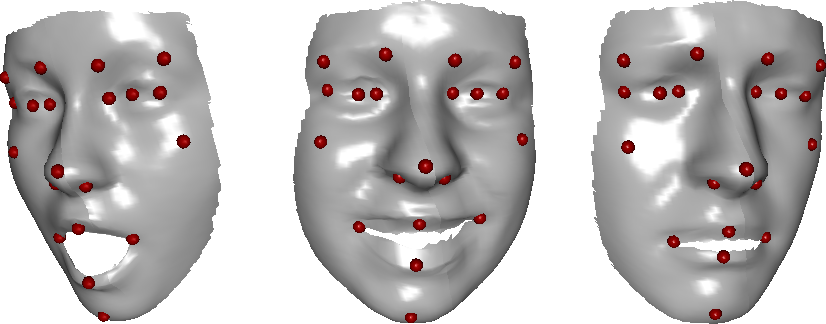
\includegraphics[scale=0.40]{images/featurePoints.png}
\par\end{centering}

\caption{Three newly generated faces with twenty feature points (denoted by the
  red spheres). These feature points define the correspondence between the model
  and the image.}
\label{fg:featurePoints}
\end{figure}

The user selects the feature points simply by clicking on the correct pixel in
the image. During the selection process, a label guides the user and informs
him which feature point he should select next. This design is shown in figure
\ref{fg:featurePoints2}.

\begin{figure}[H]
\begin{centering}
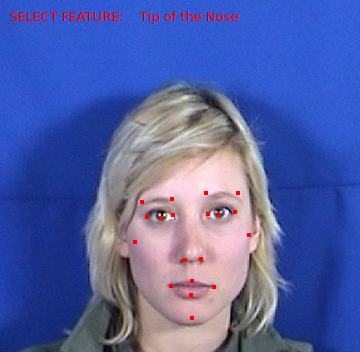
\includegraphics[scale=0.60]{images/featureSelection.png}
\par\end{centering}

\caption{The user selects points in the image which correspond to the feature
  points on the model (see figure \ref{fg:featurePoints} ).}
\label{fg:featurePoints2}

\end{figure}

How well the corresponding image feature points are selected plays a very important role
during the optimization process of the fitting algorithm. This again is due to the
sensitivity of expression estimation to detail.

\subsection{Tracking Feature Points}
After the user (or an automatic algorithm) has identified the position of the projections of model
feature points in the first frame of the recording, it is necessary to find
the positions of these points in all the successive frames. This is done
automatically using an optical flow algorithm. This algorithm attempts to
estimate the movement of the points.

The movement of points is what allows the fitting algorithm to recognize an
expression. Clearly, there are always feature points which provide more information about an
expression than
other. Points around the mouth for example are especially important for the
algorithm since most expressions are characterized by unique mouth
movements. Points on the eyebrows are also a good source of information about
the expression. Conveniently, these points are also very good for tracking since
the mouth and the eyebrows are easily distinguishable in terms of texture from
other points on the face. 

On the other hand, the features which are imperative to the recognition of a
person's identity are mostly static. These features include the distance between the
corners of the mouth, the location of the chin, the displacements between
the mouth and the nose and even the size of the eyes. The problem with feature
points which are good for estimating identity is they are often located in areas
where texture is largely constant and they are thus difficult to track. For example, selecting
feature points on the forehead or the cheeks may be crucial to determine the
measurements of the face. However, the movement of these points will be very
difficult to predict due to the lack of unique texture in their surroundings.

The Kanade-Lucas feature tracker, which was discussed in \ref{s:kanade}, is an
optical flow algorithm well suited for tracking a small number of points. A
pyramidal implementation of the Kanade-Lucas feature tracker is available in the
OpenCV library as the function \texttt{calcOpticalFlowPyrLK()}. The OpenCV
implementation is described in detail by Bouguet in \cite{kanade4}.  

Feature points may sometimes get lost during tracking process with the Kanade-Lucas
feature tracker. This can happen if the
texture around the point changes so drastically that it is impossible for the
algorithm to predict the point's movement. This may for instance happen to feature points
on the eye when a person blinks. There are two possible approaches to dealing
with lost points. The algorithm may for example assume that the point did not move at
all, which is a reasonable assumption for feature points on the eye. The other
possibility is to discard such points altogether. The second approach works
better with more general disturbances. Consider a situation when a hand is moving
in front of the face. It should usually take several frames for the hand to
pass. As the hand appears some points will get lost. If the algorithm assumed
their position did not change they would begin moving with the hand in the
following frames.
\subsection{Camera Parameters}
The feature points on the 3D model need to be projected into 2D so that their
difference from user selected points may be calculated. These points are projected
using a camera model. The parameters of this camera model must be obtained by calibrating the camera which
was used to capture the image. There are three main camera (intrinsic) parameters. As seen in section \ref{s:camera}, often it is preferable to use
four parameters. These are the two components of the principal point $c_x$,
$c_y$ and two parameters $f_x$ and $f_y$ which are computed from the focal
length $f$ and pixel to real world conversion values. The camera model used in
the expression transfer application is
\begin{equation}\label{eq:projective}
\gamma\begin{pmatrix}x\\y\\1\end{pmatrix}
= \begin{pmatrix}f_x&0&c_x&0\\0&f_y&c_y&0\\0&0&1&0\end{pmatrix} \begin{pmatrix}X\\Y\\Z\\1\end{pmatrix}
\end{equation}
The process of computing camera parameters is called camera calibration. There
are numerous algorithms for camera calibration. Most of them are based on first
using the camera to produce images of a pattern with a known 3D geometry. The calibration algorithm is then
provided with a set of marked points on the images which correspond to points in
the 3D geometry. A commonly used planar pattern for camera calibration is
the chessboard pattern. The feature points in the chessboard pattern image are
often chosen to be the inside corners of the chessboard squares. These can
be located automatically since they are easily distinguishable using edge and
corner detection filters. OpenCV provides the
\texttt{cvFindChessboardCorners(.)} function for this purpose.

\begin{figure}[H]
\begin{centering}
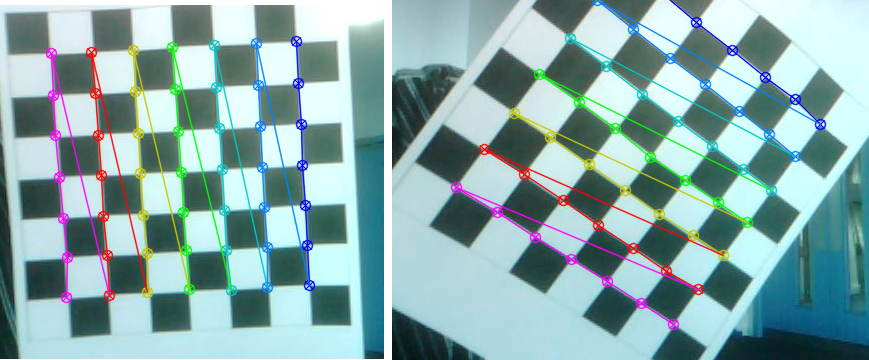
\includegraphics[scale=0.48]{images/chessboard_pattern.png}
\par\end{centering}

\caption{Locating feature points in a chessboard pattern.}
\label{fg:chessboard}

\end{figure}

The expression transfer application uses Zhang's camera calibration algorithm
\cite{zhang}. Computing the camera parameters with Zhang's algorithm requires
only a few images of a planer pattern (such as the chessboard) at different
orientations. An implementation of this algorithm is provided in OpenCV under the
function \texttt{cvCalibrateCamera(.)}. 

Utilizing OpenCV, we can thus implement camera calibration in a few steps as
\begin{itemize}
\item \textbf{Step 1.} The user inputs two or more images of a chessboard
  pattern.
\item \textbf{Step 2.} The images are processed with
  \texttt{cvFindChessboardCorners(.)} to find all the inner corners inside the
  chessboard.
\item \textbf{Step 3.} The function \texttt{cvCalibrateCamera(.)} is called with
  the found corners and with the 3D geometry of the board. This geometry need
  only be defined once when writing the algorithm.
\end{itemize}


Camera calibration can only be performed if the
user has access to the camera and can take images of a chessboard pattern. To
allow for more flexibility, it must also be possible for the user to
input camera parameters into the application manually. The GUI of the expression
transfer application therefore includes the possibility of either specifying the
parameters manually or calling the automatic calibration process. The GUI of
application provides a dialog for camera calibration. This dialog is shown in
figure \ref{fg:camdialog}

\begin{figure}[H]
\begin{centering}
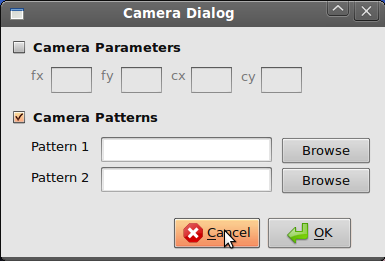
\includegraphics[scale=0.60]{images/cameraDialog.png}
\par\end{centering}

\caption{The dialog element of the expression transfer user interface, which
  allows the the user to choose between manually or automatically calibrating
  the camera.}
\label{fg:camdialog}

\end{figure}

\subsection{Minimizing the Error Function}\label{s:minerror}
The goal of the the fitting algorithm is to estimate the model and 3D pose
parameters given a set of $N$ feature points $f_1, \ldots , f_N$ in every frame of the recording. In
order to find the parameters that are closest to the true parameters we need an error
function to measure the dissimilarity between the projected 3D model and
the image. A convenient error function is the sum of squares error function
which measures this dissimilarity as the
sum of the distances between the feature points and the
projection of their corresponding 3D model points. The sum of squares
function that we need to minimize with respect to the parameters is therefore
\begin{equation}\label{eq:fit0}
E(\mathrm{parameters}) = \sum_{i=1}^N \Big\Vert\mathbf{f}_i - \mathop{proj}(\mathrm{model\; point})\Big\Vert^2
\end{equation}

The point on the model
which corresponds to the feature point $\mathbf{f}_i = (u_i,v_i)^T$ is defined as $\mathbf{p}_i = (x_i,y_i,z_i)^T$. The 3D model
points are a function of the model parameters. For the expression transfer model
this function is given by \ref{eq:gen2}. This function generates a vector
$\mathbf{X}$ which is 
obtained as a linear combination of the 3D face scans, therefore 
\begin{equation}\label{eq:fit1}
\mathbf{X} = \mathop{g}(\mathbf{w}_{id},\mathbf{w}_{exp})= \mathbf{M}_{(1)}(\mathbf{U}_{id}^T\mathbf{w}_{id} \otimes
\mathbf{U}_{exp}^T\mathbf{w}_{exp})
\end{equation}
If we were only interested in
generating 3D points as linear combinations of the 3D face scans 
then the generative function could also be specified in a more concise form by
formula \ref{eq:gen4}. However, by avoiding this simplification the weights
maintain their meaning. This meaning stems from the direct relation of the
expression and identity weights to the weight vector $\mathbf{w}$ which was used
to generate a linear combination of the columns of the flattened data
tensor as seen in equation \ref{eq:gen}. The model parameters $\mathbf{w}_{id}$
and $\mathbf{w}_{exp}$ are therefore the decomposition of the coefficients which produced this
linear combination of the data tensor columns. As such, we can impose meaningful
constraints to enforce realistic results as will be seen later. 

The components of the model point $\mathbf{p}_i$ form three successive components of the vector
$\mathbf{X}$. The point is therefore
generated by the corresponding rows from the flattened multilinear
model. We specify these row as $(\mathbf{M}_{(1)})_{i,*}$,
$(\mathbf{M}_{(1)})_{i+1,*}$ and $(\mathbf{M}_{(1)})_{i+2,*}$ respectively. To
simplify the notation these three rows collectively stacked on top of each other
will be denoted as
$[\mathbf{M}_{(1)}]_{i}$. The points $\mathbf{p}_i$ can are thus generated by the function
\begin{equation}\label{eq:fit2}
\mathbf{p}_i = \mathop{g_i}(\mathbf{w}_{id},\mathbf{w}_{exp})
= [\mathbf{M}_{(1)}]_{i}(\mathbf{U}_{id}^T\mathbf{w}_{id} \otimes \mathbf{U}_{exp}^T\mathbf{w}_{exp})
\end{equation}

In addition to the model parameters, we need
to estimate the 3D pose parameters of the 3D model so that the optimization can
account for all the degrees of freedom which available to the subject in the recording. The 3D
pose is defined by the rotation of the object and its translation. These are
specified using the rotation matrix $\mathbf{R}$ and the translation vector
$\mathbf{t}$. This rotation and translation is applied to all model points
allowing us to generate a 3D representation of any arbitrarily rotated or
 moved face. The augmented generative function is thus

\begin{equation}\label{eq:fit3}
\mathbf{p}_i = \mathop{g_i}(\mathbf{w}_{id},\mathbf{w}_{exp},\mathbf{R},\mathbf{t})
= \mathbf{R}[\mathbf{M}_{(1)}]_{i}(\mathbf{U}_{id}^T\mathbf{w}_{id} \otimes
\mathbf{U}_{exp}^T\mathbf{w}_{exp}) + \mathbf{t}
\end{equation}

Lastly, to measure the dissimilarity between the feature points $\mathbf{f}_i$ and the
corresponding 3D model points $\mathbf{p}_i$ it is necessary to project the model points
into 2D. This projection is done using the perspective camera model with a
camera matrix $\mathbf{P}$ which consists of the calibrated (or
user provided) intrinsic parameters $f_x$, $f_y$, $c_x$ and $c_y$. The result of
projecting the model point $\mathbf{p}_i$ is 
\begin{equation}\label{eq:fit5}
\gamma\begin{pmatrix}\mathbf{f}_i\\1\end{pmatrix}
= \begin{pmatrix}f_x&0&c_x\\0&f_y&c_y\\0&0&1\end{pmatrix}\mathbf{p}_i
    = \mathbf{P}\mathbf{p}_i
\end{equation}

Given the augmented generative function $\mathop{g}_i$ and the projection matrix we can now expand the
sum of square error function \ref{eq:fit0} to obtain
\begin{equation}\label{eq:fit6}
E(\mathbf{w}_{id}, \mathbf{w}_{exp}, \mathbf{R}, \mathbf{t}) = \sum_{i=1}^N \Big\Vert\begin{pmatrix}\mathbf{f}_i\\1\end{pmatrix} - \frac{1}{\gamma}\mathbf{P}\mathop{g_i}(\mathbf{w}_{id},\mathbf{w}_{exp},\mathbf{R},\mathbf{t})\Big\Vert^2
\end{equation}
The generative function can be further expanded to give
\begin{align}\label{eq:fit7}
E(\mathbf{w}_{id}, \mathbf{w}_{exp}, \mathbf{R}, \mathbf{t}) &= \sum_{i=1}^N \Big\Vert\begin{pmatrix}\mathbf{f}_i\\1\end{pmatrix} - \frac{1}{\gamma}\mathbf{P}\bigr[\mathbf{R}[\mathbf{M}_{(1)}]_{i}(\mathbf{U}_{id}^T\mathbf{w}_{id} \otimes
\mathbf{U}_{exp}^T\mathbf{w}_{exp}) + \mathbf{t}\bigl]\Big\Vert^2\\\label{eq:fit8}
&=\sum_{i=1}^N \Big\Vert\begin{pmatrix}\mathbf{f}_i\\1\end{pmatrix} - \frac{1}{\gamma}\mathbf{P}\mathbf{R}[\mathbf{M}_{(1)}]_{i}(\mathbf{U}_{id}^T\mathbf{w}_{id} \otimes
\mathbf{U}_{exp}^T\mathbf{w}_{exp}) - \frac{1}{\gamma}\mathbf{P}\mathbf{t}\Big\Vert^2
\end{align}

The optimal values of the error function parameters $\mathbf{w}_{id}$, $\mathbf{w}_{exp}$,
$\mathbf{R}$ and $\mathbf{t}$ can be obtained by setting the derivative of the
error function with respect to the parameter in question to zero and then
solving the resulting equation. These optimal parameters describe a model that
gives the smallest possible error between its projection and the image feature points.


However, the problem with the perspective projection is that to obtain the feature point
we need to dehomogenize the result of the projection by dividing with
$\gamma$. This $\gamma$ will be equal to the unknown value of the $z$-component of the point
which is being projected using the camera matrix, making the scaling factor $\gamma$ a function of the model parameters and the rotation
matrix given by $\gamma(\mathbf{w}_{id},\mathbf{w}_{exp},\mathbf{R},\mathbf{t})$. The
  perspective projection is therefore ill-suited for optimization, because the derivative of the error function will be
a nonlinear function depending on the partial derivatives of the function
$\gamma(\mathbf{w}_{id},\mathbf{w}_{exp},\mathbf{R},\mathbf{t})$. Setting the derivative to
  zero would then result in a nonlinear equation which are difficult to solve.

The presence of the scaling factor means that the perspective projection is not a linear transformation since $\gamma$ is a
function of the point $p_i$. The weak-perspective projection however is a linear
transformation and it may be used to approximate the perspective projection. The idea
behind the weak-perspective projection is that when the distance of the object
from the camera is large enough then the points on the object can be thought to have effectively same
$z$-component. Fortunately, the points on a face are very close to each other in depth, which justifies using the weak-perspective camera model as an approximation
of the perspective camera model in the fitting algorithm. 

The weak-perspective projection uses the same parameters $f_x$, $f_y$, $c_x$ and
$c_y$ as the perspective camera model. Unlike the perspective model however, the
result is divided by the average depth $z_{avg}$ of the model instead of
$\gamma$. The average depth is essentially the average $\gamma$ value of all points
in the object. The weak-perspective camera model is defined by the camera matrix
$\mathbf{P}_w$ as 

\begin{equation}\label{eq:fit9}
 \mathbf{f}_i = \frac{1}{z_{avg}}\begin{pmatrix}f_x&0&c_x\\0&f_y&c_y\end{pmatrix}\mathbf{p}_i
    = \frac{1}{z_{avg}}\mathbf{P}_w\mathbf{p}_i
\end{equation}\\
For the weak-perspective projection to provide a reasonable approximation of the
perspective projection, the points must be far enough from the origin so that
the differences in their depth are small in comparison to this distance. If this condition is not fulfilled, it is
possible to still make the weak-perspective approximation acceptable by
increasing the distance from the origin to the
image plane (defined by the focal length $f$). Increasing the focal length
is essentially equivalent to moving the object in the $z$ direction.


\paragraph{Error function.} With the weak-perspective camera model we can now define the error function for
the tensor-based model fitting algorithm as
\begin{equation}\label{eq:fit10}
E(\mathbf{w}_{id}, \mathbf{w}_{exp}, \mathbf{R}, \mathbf{t}) = \sum_{i=1}^N \Big\Vert\mathbf{f}_i - \frac{1}{z_{avg}}\mathbf{P}_w\Big(\mathbf{R}[\mathbf{M}_{(1)}]_{i}(\mathbf{U}_{id}^T\mathbf{w}_{id} \otimes
\mathbf{U}_{exp}^T\mathbf{w}_{exp}) + \mathbf{t}\Big)\Big\Vert^2
\end{equation}
which uses the weak-perspective camera matrix $\mathbf{P}_w$ to project the
rotated model point and the translation vector $t$. 

Given the error defining function $E(\mathbf{w}_{id}, \mathbf{w}_{exp}, \mathbf{R},
\mathbf{t})$, the goal is to find the optimal parameters $\mathbf{w}_{id}^*$,
$\mathbf{w}_{exp}^*$, $\mathbf{R}^*$ and
$\mathbf{t}^*$ which minimize this
error. The minimum can be found by setting the partial derivatives to zero as

\begin{align}\label{eq:fit11}
\frac{\partial E}{\partial \mathbf{w}_{id}} &= \mathbf{0} \: \mathrm{, } \: & \frac{\partial
  E}{\partial \mathbf{w}_{exp}} &= \mathbf{0}  \: \mathrm{, } \:  & \frac{\partial E}{\partial
  \mathbf{R}} &= \mathbf{0}  \: \mathrm{, } \:  & \frac{\partial E}{\partial \mathbf{t}} &= \mathbf{0}
\end{align}

The resulting equations are unfortunately nonlinear due to the square in the error
function. Consider the derivative with respect to the identity parameters given by 
\begin{align*}\label{eq:fit12}
\frac{\partial E}{\partial \mathbf{w}_{id}} &= \frac{\partial}{\partial \mathbf{w}_{id}}\sum_{i=1}^N \Big\Vert\mathbf{f}_i - \frac{1}{z_{avg}}\mathbf{P}_w\mathbf{R}[\mathbf{M}_{(1)}]_{i}\overbrace{(\mathbf{U}_{id}^T\mathbf{w}_{id} \otimes
\mathbf{U}_{exp}^T\mathbf{w}_{exp})}^{\mathbf{Z}} - \frac{1}{z_{avg}}\mathbf{P}_w\mathbf{t}\Big\Vert^2\\
&=\sum_{i=1}^N \frac{\partial}{\partial \mathbf{w}_{id}}\Big\Vert\mathbf{f}_i - \frac{1}{z_{avg}}\mathbf{P}_w\mathbf{R}[\mathbf{M}_{(1)}]_{i}\mathbf{Z} -
\frac{1}{z_{avg}}\mathbf{P}_w\mathbf{t}\Big\Vert^2\\
&=\sum_{i=1}^N -\frac{2}{z_{avg}}\Bigl(\frac{\partial \mathbf{P}_w\mathbf{R}[\mathbf{M}_{(1)}]_{i}\mathbf{Z}}{\partial
  \mathbf{w}_{id}}\Bigr)\Bigl(\mathbf{f}_i -
\frac{1}{z_{avg}}\mathbf{P}_w\mathbf{R}[\mathbf{M}_{(1)}]_{i}\mathbf{Z} -
\frac{1}{z_{avg}}\mathbf{P}_w\mathbf{t}\Bigr)
\end{align*}
where the chain rule of matrix calculus was used. 

The order of the derivations in the chain rule for vectors depends on whether the gradient is a row or column
vector. Here we will adopt the notation that the gradient is a row vector. The
chain rule is therefore ``build toward the left'' \cite{ifemcolorado}. For example, if $\mathbf{w}$
is a function of $\mathbf{z}$, which is a function of $\mathbf{y}$, which is a
function of $\mathbf{x}$ then the derivative of $\mathbf{w}$ with respect to
$\mathbf{x}$ is computed using the chain rule as
\begin{equation*}
\frac{\partial \mathbf{w}}{\partial \mathbf{x}} = \frac{\partial
  \mathbf{y}}{\partial \mathbf{x}}\frac{\partial \mathbf{z}}{\partial
  \mathbf{y}}\frac{\partial \mathbf{w}}{\partial \mathbf{z}} 
\end{equation*}
which is reverse order of the scalar chain rule where multiplication is
commutative.

The derivative of a vector function $\mathbf{A}\mathbf{x}$ with respect to a
vector $\mathbf{x}$ is defined as
\begin{equation*}
\frac{\partial \mathbf{A}\mathbf{x}}{\partial \mathbf{x}} = \mathbf{A}^T
\end{equation*}\\
Using the chain rule and then expanding $\mathbf{Z}$ we obtain
\begin{align}
\frac
{\partial 
\mathbf{P}_w\mathbf{R}[\mathbf{M}_{(1)}]_{i}\mathbf{Z}
}
{\partial
\mathbf{w}_{id}
}
&= 
\frac
{\partial
\mathbf{P}_w\mathbf{R}[\mathbf{M}_{(1)}]_{i}(\mathbf{U}_{id}^T\mathbf{w}_{id}
\otimes \mathbf{U}_{exp}^T\mathbf{w}_{exp})
}
{
\partial
\mathbf{w}_{id}
}\nonumber\\
&=
\frac
{\partial
\mathbf{U}_{id}^T\mathbf{w}_{id}
}
{\partial
\mathbf{w}_{id}
}
\frac
{\partial
(\mathbf{U}_{id}^T\mathbf{w}_{id} \otimes \mathbf{U}_{exp}^T\mathbf{w}_{exp})
}
{\partial
\mathbf{U}_{id}^T\mathbf{w}_{id}
}
\frac
{\partial
\mathbf{P}_w\mathbf{R}[\mathbf{M}_{(1)}]_{i}(\mathbf{U}_{id}^T\mathbf{w}_{id} \otimes \mathbf{U}_{exp}^T\mathbf{w}_{exp})
}
{\partial
(\mathbf{U}_{id}^T\mathbf{w}_{id} \otimes \mathbf{U}_{exp}^T\mathbf{w}_{exp})
}\nonumber\\\label{eq:opt0}
&=\mathbf{U}_{id}
\underbrace{
\frac
{\partial
(\mathbf{U}_{id}^T\mathbf{w}_{id} \otimes \mathbf{U}_{exp}^T\mathbf{w}_{exp})
}
{\partial
\mathbf{U}_{id}^T\mathbf{w}_{id}
}
}_{\mathbf{W}}
(\mathbf{P}_w\mathbf{R}[\mathbf{M}_{(1)}]_{i})^T
\end{align}
Computing the $\mathbf{W}$ requires us to take the derivative of a Kronecker
product. In \cite{matcalc} the derivative of the Kronecker of a $m \times n$
matrix $\mathbf{A}$ and a $p \times q$
matrix $\mathbf{B}$ with respect to the
matrix $\mathbf{A}$ is defined as  
\begin{equation}
\frac{\partial \mathbf{A} \otimes \mathbf{B}}{\partial \mathbf{A}} = 
\bigr(\mathbf{I}_{n} \otimes \mathop{vec}(\mathbf{B}) \otimes
\mathbf{I}_{m}\bigl)\bigr(\mathbf{I}_{nq} \otimes \mathbf{T}_{pm}\bigl)
\end{equation}
where $\mathbf{I}_{n}$ is the $n \times n$ identity matrix, $\mathop{vec}$ a
vectorization operator which stacks the columns of the operand into a vector and $\mathbf{T}_{pm}$
a $p \times m$ permutation matrix called the transpose matrix. This permutation matrix $\mathbf{T}_{pm}$ has
the special property that it reverses the Kronecker product.
\begin{equation}
\mathbf{B} \otimes \mathbf{A} = \mathbf{T}_{pm}(\mathbf{A} \otimes
\mathbf{B})\mathbf{T}_{nq}
\end{equation}\\
However, since we are taking the derivation of the Kronecker product with
respect to a vector, we can utilize the fact that the operands are vectors to simplify the equation $\mathbf{Z} =
\mathbf{U}_{id}^T\mathbf{w}_{id} \otimes
\mathbf{U}_{exp}^T\mathbf{w}_{exp}$ using the relationship between
multiplication and the Kronecker product given by 
\begin{equation*}
(A \otimes B)(C \otimes D) = (AC \otimes BD)
\end{equation*}
The expression $\mathbf{U}_{exp}^T\mathbf{w}_{exp}$ is a $I_{exp} \times
1$ matrix (or in other words a vector) which is a constant when
taking the derivation with respect to $\mathbf{w}_{id}$. We can therefore
substitute the vector $\mathbf{a} = \mathbf{U}_{exp}^T\mathbf{w}_{exp}$ into $\mathbf{Z}$
to get 
\begin{align}
\mathbf{Z} &= \mathbf{U}_{id}^T\mathbf{w}_{id} \otimes
\mathbf{U}_{exp}^T\mathbf{w}_{exp}\nonumber\\
& = \mathbf{U}_{id}^T\mathbf{w}_{id} \otimes
\mathbf{a}\nonumber\\
&= \mathbf{I}_{I_{id}}\mathbf{U}_{id}^T\mathbf{w}_{id} \otimes
\mathbf{a}\mathbf{I}_1 \nonumber\\
&= (\mathbf{I}_{I_{id}} \otimes \mathbf{a})(\mathbf{U}_{id}^T\mathbf{w}_{id}
\otimes \mathbf{I}_1)\nonumber\\
\label{eq:opt1}
&=(\mathbf{I}_{I_{id}} \otimes \mathbf{U}_{exp}^T\mathbf{w}_{exp})\mathbf{U}_{id}^T\mathbf{w}_{id}
\end{align}
since $\mathbf{I}_1 = 1$. Using a similar approach it is also possible to extract
$\mathbf{w}_{exp}$ out of $\mathbf{Z}$ to obtain
\begin{equation}\label{eq:opt2}
\mathbf{U}_{id}^T\mathbf{w}_{id} \otimes
\mathbf{U}_{exp}^T\mathbf{w}_{exp} = (\mathbf{U}_{id}^T\mathbf{w}_{id} \otimes
\mathbf{I}_{I_{exp}})\mathbf{U}_{exp}^T\mathbf{w}_{exp} 
\end{equation}
With this result we can now evaluate $\mathbf{W}$ to obtain
\begin{align*}
\mathbf{W} &= 
\frac
{\partial
(\mathbf{U}_{id}^T\mathbf{w}_{id} \otimes \mathbf{U}_{exp}^T\mathbf{w}_{exp})
}
{\partial
\mathbf{U}_{id}^T\mathbf{w}_{id}
}= 
\frac
{\partial
(\mathbf{I}_{I_{id}} \otimes \mathbf{U}_{exp}^T\mathbf{w}_{exp})\mathbf{U}_{id}^T\mathbf{w}_{id}
}
{\partial
\mathbf{U}_{id}^T\mathbf{w}_{id}
}\\
&=(\mathbf{I}_{I_{id}} \otimes
\mathbf{U}_{exp}^T\mathbf{w}_{exp})^T =(\mathbf{I}_{I_{id}} \otimes
\mathbf{w}_{exp}^T\mathbf{U}_{exp})
\end{align*}
This result, obtained using \ref{eq:opt1}, adheres with the derivation of
the Kronecker product, since for transpose matrices it holds that $\mathbf{T}_{n1} =
\mathbf{T}_{1n} = \mathbf{I}_n$ for any $n$.\\
\\
With the known $\mathbf{W}$ we can complete the derivation we began in \ref{eq:opt0} to get
\begin{align}
\frac
{\partial 
\mathbf{P}_w\mathbf{R}[\mathbf{M}_{(1)}]_{i}\mathbf{Z}
}
{\partial
\mathbf{w}_{id}
}
&=\mathbf{U}_{id}
\frac
{\partial
(\mathbf{U}_{id}^T\mathbf{w}_{id} \otimes \mathbf{U}_{exp}^T\mathbf{w}_{exp})
}
{\partial
\mathbf{U}_{id}^T\mathbf{w}_{id}
}
(\mathbf{P}_w\mathbf{R}[\mathbf{M}_{(1)}]_{i})^T\nonumber\\
&=
\mathbf{U}_{id}
(\mathbf{I}_{I_{id}} \otimes
\mathbf{w}_{exp}^T\mathbf{U}_{exp})
[\mathbf{M}_{(1)}]_{i}^T\mathbf{R}^T\mathbf{P}_w^T
\end{align}
The results from equations \ref{eq:opt1} and \ref{eq:opt2} also allow us to decompose the Kronecker product
in the error function as well. Thus we obtain the derivation of the error function with respect to
$\mathbf{w}_{id}$ to be
\begin{align*}\label{eq:opt4}
\frac{\partial E}{\partial \mathbf{w}_{id}} &= \sum_{i=1}^N -\frac{2}{z_{avg}}\Bigl(
\frac{\partial \mathbf{P}_w\mathbf{R}[\mathbf{M}_{(1)}]_{i}\mathbf{Z}}
{\partial \mathbf{w}_{id}}\Bigr)\Bigl(\mathbf{f}_i - \frac{1}{z_{avg}}\mathbf{P}_w\mathbf{R}[\mathbf{M}_{(1)}]_{i}\mathbf{Z} - \frac{1}{z_{avg}}\mathbf{P}_w\mathbf{t}\Bigr)\\
&=\sum_{i=1}^N -\frac{2}{z_{avg}}\underbrace{\Bigl(\mathbf{U}_{id} (\mathbf{I}_{I_{id}} \otimes \mathbf{w}_{exp}^T\mathbf{U}_{exp}) [\mathbf{M}_{(1)}]_{i}^T\mathbf{R}^T\mathbf{P}_w^T\Bigr)}_{\mathbf{H}_i^T}\Bigl(\mathbf{f}_i - \frac{1}{z_{avg}}\mathbf{P}_w\mathbf{R}[\mathbf{M}_{(1)}]_{i}\mathbf{Z} - \frac{1}{z_{avg}}\mathbf{P}_w\mathbf{t}
\Bigr)\\
&= \frac{2}{z_{avg}}\sum_{i=1}^N\bigl(
\mathbf{H}_i^T\frac{1}{z_{avg}}\mathbf{P}_w\mathbf{R}[\mathbf{M}_{(1)}]_{i}\mathbf{Z}\bigr)
-
\frac{2}{z_{avg}}\sum_{i=1}^N \mathbf{H}_i^T\bigl(\mathbf{f}_i - \frac{1}{z_{avg}}\mathbf{P}_w\mathbf{t}
\bigr)\\
&=
\frac{2}{z_{avg}^2}\sum_{i=1}^N\bigl(
\mathbf{H}_i^T\underbrace{\mathbf{P}_w\mathbf{R}[\mathbf{M}_{(1)}]_{i}(\mathbf{I}_{I_{id}} \otimes \mathbf{U}_{exp}^T\mathbf{w}_{exp})\mathbf{U}_{id}^T}_{\mathbf{H}_i}\mathbf{w}_{id}\bigr)
-
\frac{2}{z_{avg}}\sum_{i=1}^N \mathbf{H}_i^T\bigl(\mathbf{f}_i -
\frac{1}{z_{avg}}\mathbf{P}_w\mathbf{t}\bigr)\\
&=\frac{2}{z_{avg}^2}\sum_{i=1}^N\bigl(
\mathbf{H}_i^T\mathbf{H}_i\mathbf{w}_{id}\bigr)
-
\frac{2}{z_{avg}}\sum_{i=1}^N \mathbf{H}_i^T\bigl(\mathbf{f}_i -
\frac{1}{z_{avg}}\mathbf{P}_w\mathbf{t}\bigr)
\end{align*}
To find the optimal identity parameters $\mathbf{w}_{id}^*$ which minimize the error function we set
this derivative to zero to obtain the system of equations 
\begin{align*}
&\frac{2}{z_{avg}^2}\sum_{i=1}^N\bigl(
\mathbf{H}_i^T\mathbf{H}_i\mathbf{w}^*_{id}\bigr)
-
\frac{2}{z_{avg}}\sum_{i=1}^N \mathbf{H}_i^T\bigl(\mathbf{f}_i -
\frac{1}{z_{avg}}\mathbf{P}_w\mathbf{t}^*\bigr) = 0\\
&\frac{2}{z_{avg}^2}\sum_{i=1}^N\bigl(
\mathbf{H}_i^T\mathbf{H}_i\mathbf{w}^*_{id}\bigr)
=
\frac{2}{z_{avg}}\sum_{i=1}^N \mathbf{H}_i^T\bigl(\mathbf{f}_i -
\frac{1}{z_{avg}}\mathbf{P}_w\mathbf{t}^*\bigr)\\
&\frac{1}{z_{avg}}\sum_{i=1}^N\bigl(
\mathbf{H}_i^T\mathbf{H}_i\mathbf{w}^*_{id}\bigr)
=
\sum_{i=1}^N \mathbf{H}_i^T\bigl(\mathbf{f}_i -
\frac{1}{z_{avg}}\mathbf{P}_w\mathbf{t}^*\bigr)\\
\end{align*}
This system of equations can be written in matrix form as
\begin{equation}
\frac{1}{z_{avg}}\mathbf{H}^T\mathbf{H}\mathbf{w}^*_{id} =
\mathbf{H}^T\bigl(\mathbf{f} - \frac{1}{z_{avg}}\mathbf{P}_w\mathbf{t}^*\bigr)
\end{equation}
with
\begin{equation}
\mathbf{H} = 
\begin{pmatrix}
\mathbf{H}_1\\
\mathbf{H}_2\\
\vdots\\
\mathbf{H}_N
\end{pmatrix}
\quad \mathrm{and} \quad 
\mathbf{f} = 
\begin{pmatrix}
\mathbf{f}_1\\
\mathbf{f}_2\\
\vdots\\
\mathbf{f}_N
\end{pmatrix}
\end{equation}
The solution of this system of equations in matrix form is the optimal identity parameter
vector $\mathbf{w}^*_{id}$ which is given by
\begin{equation}\label{eq:nonlin1}
\mathbf{w}^*_{id} = z_{avg}(\mathbf{H}^T\mathbf{H})^{-1}\mathbf{H}^T\bigl(\mathbf{f} - \frac{1}{z_{avg}}\mathbf{P}_w\mathbf{t}^*\bigr)
\end{equation}
with
\begin{equation}\label{eq:H}
\mathbf{H}_i = \mathbf{P}_w\mathbf{R}^*[\mathbf{M}_{(1)}]_{i}(\mathbf{I}_{I_{id}}
\otimes \mathbf{U}_{exp}^T\mathbf{w}^*_{exp})\mathbf{U}_{id}
\end{equation}
The optimal expression parameter vector $\mathbf{w}^*_{exp}$ is obtained in the
same manner by setting the derivative of the error function with respect to
$\mathbf{w}^*_{exp}$ to zero. The result is 
\begin{equation}\label{eq:nonlin2}
\mathbf{w}^*_{exp} = z_{avg}(\mathbf{G}^T\mathbf{G})^{-1}\mathbf{G}^T\bigl(\mathbf{f} - \frac{1}{z_{avg}}\mathbf{P}_w\mathbf{t}^*\bigr)
\end{equation}
with 
\begin{equation}\label{eq:G}
\mathbf{G}_i =
\mathbf{P}_w\mathbf{R}^*[\mathbf{M}_{(1)}]_{i}(\mathbf{U}_{id}^T\mathbf{w}^*_{id}
\otimes \mathbf{I}_{I_{exp}})\mathbf{U}_{exp}
\end{equation}
From equations \ref{eq:nonlin1} and \ref{eq:nonlin2} we see that solving for
the optimal parameters reduces to a system of nonlinear equations. Both the
$\mathbf{w}^*_{exp}$ and $\mathbf{w}^*_{id}$ depend on the other optimal parameter vector as
well as on the optimal rotation matrix $\mathbf{R}^*$ and the optimal translation
vector $\mathbf{t}^*$, which are likewise obtained by setting the respective
derivative to zero. The resulting nonlinear system may be solved using a Newton or
quasi-Newton optimization method to obtain approximations to these optimal solutions.

\paragraph{Coordinate-Descent Method}
Instead of approximating the solution using a Newton optimization method, it is
possible to linearize the nonlinear system by fixing each of the parameters
except for one to their current guesses. Only the one free parameter is thereby
allowed to vary. The resulting linear system is then solved
to give a new guess for the free parameter. In the next iteration, this free parameter is then fixed to
this new guess and the process is restarted on one of the other parameters. The cycle
is repeated until convergence. This approach is known as minimization by coordinate
descent \cite{Press1992}. Coordinate-descent was also used by Vlasic et al in \cite{faceTransfer05}
to approximate the optimal parameters of a tensor model during each iteration of
the Kanade-Lucas feature tracker.

Newton's method may not converge if the starting point is far from the
optimum. Therefore to avoid using the Newton's method on a nonlinear system, we
minimize the expression transfer error function (\ref{eq:fit10}) using
a coordinate-descent method which combines the equations
\ref{eq:nonlin1}, \ref{eq:nonlin2} with the POSIT algorithm discussed in section
\ref{posit}. An implementation of the POSIT algorithm is available in OpenCV as
the function \texttt{solvePnP(.)}. As arguments, the function requires a camera matrix, a set of image
feature points and the corresponding model points which can be generated from
the model identity and expression parameters using equation \ref{eq:gen4}.

The optimization algorithm is initialized with a guess for the
model parameters $\mathbf{w}_{exp}$ and $\mathbf{w}_{id}$ which correspond
to a realistic face. Using this guess, the POSIT algorithm estimates a rotation
matrix and a translation vector. Given the estimated 3D pose, first the
expression is updated using equation \ref{eq:nonlin2}. Then the updated guess
for $\mathbf{w}_{exp}$ is used to solve equation \ref{eq:nonlin1} to give a new
guess for the identity parameters $\mathbf{w}_{id}$. The updated model
parameters are the used to generate a new face using equation
\ref{eq:gen4}. The updated face is then used to update the 3D pose using
the POSIT algorithm, completing one iteration of the algorithm. The iterations are repeated until convergence. The values $\mathbf{\hat{w}}_{exp}$, $\mathbf{\hat{w}}_{exp}$,
$\mathbf{\hat{R}}$ and $\mathbf{\hat{t}}$ of the parameters at convergence
approximate the values of the optimal parameters.

One issue with this approach lies in the average depth $z_{avg}$. The value of
$z_{avg}$ must be an average of the rotated and translated object's depth. This
value is therefore only available once both the 3D pose and the model
parameters have been computed.

There are two ways to deal with the $z_{avg}$ problem. One way is to assume that
$z_{avg}$ is just another parameter of the model and then update it during the coordinate
descent minimization until at termination the sequence of $z_{avg}$ guesses
converges to the true average depth. The $z_{avg}$ guess is easily obtained
after performing the POSIT update by averaging the rotated and translated generated points.

The second approach is to move the $z_{avg}$ into the model parameters. Since
the average depth is a constant we can simply scale the model parameters with
this constant to obtain the scaled parameters $\mathbf{\tilde{w}}^*_{exp}$,
$\mathbf{\tilde{w}}^*_{exp}$ as
\begin{align*}
\mathbf{\tilde{w}}^*_{exp} = \frac{1}{z_{avg}}\mathbf{w}^*_{exp} \quad
\textrm{and} \quad
\mathbf{\tilde{w}}^*_{id} = \frac{1}{z_{avg}}\mathbf{w}^*_{id}
\end{align*}
We then attempt to approximate these scaled model parameters during the
coordinate-descent without needing to worry about average depth.

The advantage of the second approach is that it decreases the number of steps in
the algorithm. However, the disadvantage is that the scaled parameter vector may
be scaled with perhaps a negative value which may cause difficulties during constrained
optimization when constraints are enforced on the parameter vectors. To keep the
optimization as general as possible the expression transfer application
therefore utilizes the first approach.

The expression transfer coordinate-descent method for one frame is thus
\begin{algorithm}\label{a:coorddesc}
\caption{Coordinate-descent for one frame}
\begin{algorithmic}[1]
\Procedure{CoordDesc}{$f_1, \ldots ,f_N$, $[\mathbf{M}_{(1)}]_{1} \ldots ,
  [\mathbf{M}_{(1)}]_{N}$, $\mathbf{P}_w$} 

\State \textbf{Output} $\mathbf{\hat{w}}_{id}$, $\mathbf{\hat{w}}_{exp}$,
$\mathbf{\hat{R}}$ and $\mathbf{\hat{t}}$
\State \textbf{Initialization} $\mathbf{\hat{w}}_{id} = [0,0, \ldots 1, \ldots
  ,0]^T$, $\mathbf{\hat{w}}_{exp} = [0,0, \ldots 1, \ldots ,0]^T$
\Repeat

\State $\mathbf{X} = \mathbf{M}_{(1)}(\mathbf{w}_{id} \otimes \mathbf{w}_{exp})$ 

\State $\mathbf{\hat{R}}$, $\mathbf{\hat{t}} \gets $
\texttt{opencv.solvePnP}($f_1, \ldots ,f_N$,$\mathbf{X}$, $\mathbf{P}_w$)

\State

\State $z_{avg} \gets$ \texttt{z-mean}($\mathbf{\hat{R}}\mathbf{X} + \mathbf{\hat{t}}$)

\State

\State $\mathbf{G}_i = \mathbf{P}_w\mathbf{\hat{R}}[\mathbf{M}_{(1)}]_{i}(\mathbf{U}_{id}^T\mathbf{\hat{w}}_{id}
\otimes \mathbf{I}_{I_{exp}})\mathbf{U}_{exp}$
\State $\mathbf{G} \gets $ \texttt{stack-horizontally}($\mathbf{G}_i$)
\State
\State $\mathbf{\hat{w}}_{exp} = z_{avg}(\mathbf{G}^T\mathbf{G})^{-1}\mathbf{G}^T\bigl(\mathbf{f} - \frac{1}{z_{avg}}\mathbf{P}_w\mathbf{\hat{t}}\bigr)$
\State
\State $\mathbf{H}_i = \mathbf{P}_w\mathbf{\hat{R}}[\mathbf{M}_{(1)}]_{i}(\mathbf{I}_{I_{id}}
\otimes \mathbf{U}_{exp}^T\mathbf{\hat{w}}_{exp})\mathbf{U}_{id}$
\State $\mathbf{H} \gets $ \texttt{stack-horizontally}($\mathbf{H}_i$)
\State
\State $\mathbf{\hat{w}}_{id} = z_{avg}(\mathbf{H}^T\mathbf{H})^{-1}\mathbf{H}^T\bigl(\mathbf{f} - \frac{1}{z_{avg}}\mathbf{P}_w\mathbf{\hat{t}}\bigr)$

\Until stopping criteria fulfilled

\EndProcedure
\end{algorithmic}
\end{algorithm}

\subsection{Overfitting}\label{s:overfitting}
As pointed out earlier the generative model only generates realistic
representations of a face when the model parameters are within several standard
deviations of the mean. In \cite{blanz1}, \cite{jacey} the model parameters are constrained to
be in the range of $\pm$3 standard deviations for the PCA based model. However, the upper and
lower bound are not known in the tensor-based shape model utilized by the
expression transfer application. 

So that the application generates believable results, the optimization through coordinate-descent
should find only model parameters that represent a realistic face. The optimal
parameters $\mathbf{w}^*_{exp}$, $\mathbf{w}^*_{id}$, $\mathbf{R}^*$ and
$\mathbf{t}^*$ obtained through minimization of the error function may not be realistic. This is due to the fact that the model may not
be able to generate any arbitrary face if it is not present in the database. The model
can only build linear combinations of the faces in the database. A face present
in the image may not be obtainable as this linear combination. In such a case the
optimal model parameters which minimize the error will therefore not be the parameters
of the optimal face. Instead they will be the parameters of the one shape which
minimizes the error for the feature points $f_1, \ldots f_N$. If this shape is
more than a few standard deviations from the mean it not resemble a face. 

This problem is well known to machine learning
where it is known as \textit{overfitting}. The minimization finds the parameters
of a shape which is too specific, because it minimizes the error for a specific set of
feature points. However, since the model parameters are too specific they cause
a large error for other points on the image which were not used to fit the
model. 

The model fitting algorithm should therefore be \textit{general} enough so that
the obtained model parameters minimize the error function not only for the feature points used during the fitting stage, but also for any
arbitrary point on the face. This can be achieve trivially by increasing the
number of feature points. Such an approach is however error prone since it is not
always clear how many points is enough to make the fitting general. 

The expression transfer application supports two techniques which ensure that the
fitting algorithm generates realistic faces. They are \textit{regularization}
and \textit{constrained minimization}.

\paragraph{Regularization.}
As discussed, unrealistic faces are produced when the model parameters are far
from the mean. To manipulate the minimization to prefer parameters which are
close to the mean we can add a regularization term to the error function. A reasonable choice for this term is
one which penalizes the distance of the parameters from their respective mean.
The augmented error function is then given by
\begin{equation}\label{eq:regular}
E = \sum_{i=1}^N \Big\Vert\mathbf{f}_i - \frac{1}{z_{avg}}\mathbf{P}_w\mathbf{R}[\mathbf{M}_{(1)}]_{i}(\mathbf{U}_{id}^T\mathbf{w}_{id} \otimes
\mathbf{U}_{exp}^T\mathbf{w}_{exp}) + \mathbf{t}\Big\Vert^2
+ \frac{\lambda}{2}\begin{Vmatrix}\mathbf{w}_{id} - \mathbf{\bar{w}}_{id}\\\mathbf{w}_{exp} - \mathbf{\bar{w}}_{exp}\end{Vmatrix}^2
\end{equation}
where $\mathbf{\bar{w}}_{exp}$ is the mean expression parameter vector and
$\mathbf{\bar{w}}_{id}$ the mean identity parameter vector. The parameter
$\lambda$ is the regularization parameter. By increasing $\lambda$ the fitting
algorithm is made more general, by decreasing $\lambda$ it is made more
specific. 

Setting the partial derivatives with respect to identity and expression of
\ref{eq:regular} to zero and solving gives us the following update equations for
the model parameters
\begin{align}
\mathbf{w}^*_{id} &=z_{avg}(\mathbf{H}^T\mathbf{H} + \lambda\mathbf{I}_{id})^{-1}\mathbf{H}^T\bigl(\mathbf{f}
- \frac{1}{z_{avg}}\mathbf{P}_w\mathbf{t}^*\bigr) + \lambda z_{avg}\mathbf{\bar{w}}_{id}\\
\mathbf{w}^*_{exp} &=z_{avg}(\mathbf{G}^T\mathbf{G} + \lambda\mathbf{I}_{exp})^{-1}\mathbf{G}^T\bigl(\mathbf{f} -
\frac{1}{z_{avg}}\mathbf{P}_w\mathbf{t}^*\bigr) + \lambda z_{avg}\mathbf{\bar{w}}_{exp}
\end{align}
with the matrices $\mathbf{H}$ and $\mathbf{G}$ unchanged.

\paragraph{Constrained Optimization.} Regularization suffers from the fact that
the optimal value of regularization parameter $\lambda$ must be found either
manually by the user or using prior knowledge about the distribution of the
parameters. Ideally, we would like to obtain a technique that does not depend on
the value of $\lambda$.

The fundamental problem is that the linear
combination of the original face scans may generate non-realistic faces. However, with a linear interpolation of
the original faces it is always the case that a realistic face is
generated. This is because linear interpolation produces faces from the convex hull spanned by
faces in the database. At the center of this convex hull is the mean. On the
sides, the hull
is bounded by the original faces. Therefore any face inside this hull consists
of points which are interpolations of the points on the original faces. With linear interpolation the fitting algorithm is able to generate realistic faces without needing to resort to regularization.

To ensure that we obtain a linear interpolation we must enforce constraints on
the model parameters. For both the identity and the expression parameter vector
it must hold that all the components are greater or equal to zero and
that they sum to one. The constrained minimization problem that the fitting
algorithm must solve is therefore given by
\begin{align}\label{eq:optprob}
\mathrm{minimize}\quad &\sum_{i=1}^N \Big\Vert\mathbf{f}_i - \frac{1}{z_{avg}}\mathbf{P}_w\mathbf{R}[\mathbf{M}_{(1)}]_{i}(\mathbf{U}_{id}^T\mathbf{w}_{id} \otimes
\mathbf{U}_{exp}^T\mathbf{w}_{exp}) + \mathbf{t}\Big\Vert^2\\
\mathrm{subject\; to}\quad &\sum_{i=1}^{I_{id}} w_{id_i} = 1\\
&\sum_{i=1}^{I_{exp}} w_{exp_i} = 1\\
\label{eq:nonneg1}
&w_{id_i} \ge 0 \quad i=1,\ldots ,I_{id}\\\label{eq:nonneg2}
&w_{exp_i} \ge 0 \quad i=1,\ldots ,I_{exp}
\end{align}

Constrained minimization of a nonlinear function is a difficult task. It
involves setting up the Karush-Kuhn-Tucker conditions or the Lagrangian function
and taking the derivatives. We can however be solve the problem using the Nelder
Mead downhill simplex discussed in section \ref{s:nelder}. The downhill simplex
method does not require the derivatives. It finds the minimum by evaluating the
function at specific points in order to move towards the minimum. 

To solve a constrained optimization problem the downhill simplex method needs to
be augmented. The simplest way to do this is to make the function evaluation
return infinity when the constraints are not satisfied. 

The drawback of the downhill simplex method is that it usually performs a large
number of function evaluations. However, every evaluation amounts to computing the
error function for all feature points. The downhill simplex method is thus not
very efficient.

Experimentation showed that unrealistic faces are generated only when the
non-negativity constraints \ref{eq:nonneg1} and \ref{eq:nonneg2} are
violated. When the constraints which ensure the sum are violated then the
resulting face is merely larger but still a realistic representation. We can therefore ensure that the fitting algorithm produces only
realistic faces by solving the minimization problem \ref{eq:optprob} given only the non-negativity
conditions. The simplified constrained optimization problem is therefore  
\begin{align}
\mathrm{minimize}\quad &\sum_{i=1}^N \Big\Vert\mathbf{f}_i - \frac{1}{z_{avg}}\mathbf{P}_w\mathbf{R}[\mathbf{M}_{(1)}]_{i}(\mathbf{U}_{id}^T\mathbf{w}_{id} \otimes
\mathbf{U}_{exp}^T\mathbf{w}_{exp}) + \mathbf{t}\Big\Vert^2\\
\mathrm{subject\; to}\quad &w_{id_i} \ge 0 \quad i=1,\ldots ,I_{id}\\\
&w_{exp_i} \ge 0 \quad i=1,\ldots ,I_{exp}
\end{align}
This makes it possible to to update the identity and
expression model parameters at every iteration of the coordinate descent
algorithm using the Sequential Coordinate-wise Non-negativity
Least Squares Algorithm introduced in \ref{a:sca}. 

The reason why only non-negative parameters produce unrealistic faces is most
likely due to the fact that during the linear combination only a subtraction of
faces can produce the zero vector. The null space of the data tensor thus spans only the negative
parameter space. 

It is entirely possible to generate some realistic
faces even when the non-negativity conditions are violated, so by enforcing
these constraints the model losses expressive power. However, it is
impossible to generate an unrealistic face when they are satisfied, which
warrants enforcing the non-negativity constraints.

\subsection{Fitting Algorithm}\label{s:fitalgo}
Before the complete fitting algorithm can be established two problems need to be
addressed. 

\paragraph{Multi-Frame Coordinate Descent.} First of all the coordinate descent algorithm discussed so far was
designed to optimize the parameters for just one frame. The fitting algorithm
should however find the identity and the expressions of a person by examining a
sequence of frames. As an additional constraint, the identity parameters should
stay the same in all frames since the identity of the person in the video
sequence should not change. In the multi-frame coordinate descent algorithm we
therefore first find the expression
parameters for every frame using a guess for the identity parameters. Then we
use the feature points and the estimated expression parameter vectors collected from all frames
to solve for the identity parameters. This process can then be iteratively
repeated until convergence.

\paragraph{Feature point generation.} The second problem concerns the feature
points. To find a reasonable approximation of the expression in the
video sequence, it is necessary to use a large number of feature points. The user cannot
be expected to enter that many points. The algorithm must therefore be able to generate
a number of new points to use in addition to the feature points specified
by the user. These points cannot be picked just randomly, they must correspond
to known points on the model so that they can be used in the error
function. 

The task is thus to generate feature points which
correspond to known points on the model. This can be done by either selecting
new 3D points on the model and projecting them to generate the new feature
points in the image, or
inversely by selecting points in the 2D image and reprojecting them into 3D. When
points are projected from the model the correspondence is already given. When
they are reprojected from the image into 3D then the corresponding 3D point to the 2D image
is chosen to be the 3D point on the model which is closest
in terms of Euclidean distance to the reprojected point.

To establish the correspondence in this manner the camera matrix and the 3D pose
need to be
known. These define the projection from object coordinate space into image
space. When using a weak-perspective camera model, this projection can be inverted to give the reprojection from image space into
object coordinate space. Likewise, it is necessary to know the shape of the face in 3D space. This
shape is generated using the expression and identity parameters. So to be able
to generate new points with known correspondences we require all the unknown parameters
we are attempting to find. This is clearly a problem. The best approach is to find the 3D pose and model parameters of the
first frame by means of optimization using only the small number of user provided
feature points. These rough estimations of the parameters can then be used to
generate more points with known correspondences which are then tracked using
optical flow and used in the error function of the following frames. Finding
these parameter estimates for the first frame is known as \textit{first frame
  alignment}.

The first frame alignment approach to generating new feature points raises an
important issue. The problem lies in the fact that an estimate of the model
parameters and 3D pose is used to generate most of the feature points. These are later 
utilized to minimize the error. Thus, it is clear that with each and every newly
generated point we are influencing our result. The error for every point that was generated
using the estimates is of course minimized exactly when the parameters
assume the values of the model and 3D pose parameter estimates. Fortunately,
the fitting algorithm utilizes information obtained from the movement of these tracked
points not from their static position. Therefore, as long as the reprojected
point is not static and at least
close enough to the true model point, then this reprojected point still supports
the correct model parameters even though it does not correspond to the true
3D model point. For the reprojection to be close enough it is necessary to have
a good estimate of the rotation matrix and the translation vector. This is
because the rotation and translation account for most of the movement of points in 3D. The variation
due to the model parameters is small in comparison.


\paragraph{Expression Transfer Fitting Algorithm. } \label{s:fit}Given are $N$ image feature points $f_1, \ldots ,f_N$, the
calibrated weak perspective camera matrix $\mathbf{P}_w$ and the regularization
parameter $\lambda$. To fit the
tensor-based shape model to these point the parameters $\mathbf{w}_{id}$,
$\mathbf{w}_{exp}$, $\mathbf{R}$ and $\mathbf{t}$ are located as follows
\begin{itemize}
\item \textbf{Step 1.} Calculate the first frame alignment using the single
  frame coordinate descent algorithm \ref{a:coorddesc} optimizing with
  regularization for the $N$ feature
  points $f_1, \ldots ,f_N$ to obtain initial estimates of $\mathbf{w}_{id}$,
$\mathbf{w}_{exp}$, $\mathbf{R}$ and $\mathbf{t}$.
\item \textbf{Step 2.} Generate new $M$ points using the 3D pose and model
  parameters. Do this by uniformly sampling points in the 2D image around important
  feature like the mouth and the eyebrows to obtain new feature points $f_{N+1},
  \ldots, f_{N+M}$. Then reproject these points into 3D to obtain 3D points $p_{N+1},
  \ldots, p_{N+M}$ using 
\begin{equation*}
p_i = \mathbf{R}^T(\mathbf{P}_w^{-1}f_i - \mathbf{t})
\end{equation*}
utilizing the parameters obtained through first frame alignment. Finally
establish correspondences to model points by finding the closest 3D model point
$m_i$ to the point $p_i$ using Euclidean distance.
\item \textbf{Step 3.} Track the $N+M$ point using the Kanade-Lucas feature
  tracker (OpenCV function \texttt{calcOpticalFlowPyrLK()}), dropping lost points, to obtain $R_i \le N+M$ image feature
  points in every $i$-th frame.
\item \textbf{Step 4.} Perform the multi-frame coordinate descent algorithm by repeating
\begin{itemize}
\item[\textbullet] \textbf{Step 5.} Update the 3D pose estimates for every frame
  using the POSIT algorithm (OpenCV function \texttt{solvePnP()}).
\item[\textbullet] \textbf{Step 6.} Update the expression parameter vector
  estimate for every frame using 
\begin{equation*}
\mathbf{w}_{exp} =z_{avg}(\mathbf{G}^T\mathbf{G} + \lambda\mathbf{I}_{exp})^{-1}\mathbf{G}^T\bigl(\mathbf{f} -
\frac{1}{z_{avg}}\mathbf{P}_w\mathbf{t}\bigr) + \lambda z_{avg}\mathbf{\bar{w}}_{exp}
\end{equation*}
with 
\begin{equation*}
\mathbf{G}_i =
\mathbf{P}_w\mathbf{R}[\mathbf{M}_{(1)}]_{i}(\mathbf{U}_{id}^T\mathbf{w}_{id}
\otimes \mathbf{I}_{I_{exp}})\mathbf{U}_{exp}
\end{equation*}
\item[\textbullet] \textbf{Step 7.} Collect the feature points from all frame
  and update the identity parameter vector using 
\begin{equation*}
\mathbf{w}_{id} =z_{avg}(\mathbf{H}^T\mathbf{H} + \lambda\mathbf{I}_{id})^{-1}\mathbf{H}^T\bigl(\mathbf{f}
- \frac{1}{z_{avg}}\mathbf{P}_w\mathbf{t}\bigr) + \lambda z_{avg}\mathbf{\bar{w}}_{id}
\end{equation*}
with
\begin{equation*}
\mathbf{H}_i = \mathbf{P}_w\mathbf{R}[\mathbf{M}_{(1)}]_{i}(\mathbf{I}_{I_{id}}
\otimes \mathbf{U}_{exp}^T\mathbf{w}_{exp})\mathbf{U}_{id}
\end{equation*}
\end{itemize}
\item \textbf{Step 8.} Until convergence 
\end{itemize}
The above algorithm enforces realistic faces using
regularization. To use constrained optimization instead, it is only necessary to
change the update steps 6. and 7. so that the parameter vectors are updated using
the the Sequential Coordinate-wise Non-negativity Least Squares Algorithm given
in \ref{a:sca}.

\section{Expression Transfer}\label{s:exptranalgo}
Ideally, the expression transfer application should be able to seamlessly change
the expressions of the individual in the target video with the expressions from
the source video. This of course involves correctly generating the texture for
the respective expressions. Since the tensor model we have constructed is a
shape model and not an appearance model, it cannot be used to directly generate
the correct texture. The shape model does however provide the application with an
understanding of the source and target face. This understanding can be utilized
to transfer the texture between the target subject in the 2D frames of the
video.

The simplest way of transferring the texture between the two
video sequences is to create a texture map of the target face and then map
the texture onto the estimated 3D model of this face. The application can
construct the texture map after all the model and pose parameters have been
estimated by projecting all the model points into the image to obtain their
image coordinates. The RGB values at these image coordinates make up the texture
map's contents and the image coordinates themselves can be used as the texture
coordinates. Usually, this texture itself is captured from the first frame of the
target video sequence. If the subject has a neutral expression in the first frame and a smiling expression is
transferred onto him, then this will cause the original texture to contract and
stretch to fit the new configuration of model points. It is clear that this
approach alone cannot produce very realistic results. 

We may however utilize the information available about the target and source
face shape to generate more realistic results. If the exact measurements of the
source subject's smile and the size of the target's mouth are known then the texture
of the source smile can be transferred into the target frame and blended with its
surroundings. This blending has to be seamless so that the result appears believable. 

\paragraph{Poisson Cloning.} Realistic blending of images can be achieved using
Poisson image editing techniques. The Poisson cloning method, described by Perez
et al in \cite{perez}, and Leyvand \cite{poisson} allows for seamless cloning of
regions between images.
The method is based on the two observations. Firstly, it is known to
psychologists \cite{perez} that second-order variations, rather than
slow gradients of intensity, are most important perceptually. Secondly, a scalar
function is uniquely defined by its Laplacian and the values at its
boundary. Since the Laplacian of an image filters everything but the second
order variations in intensity, we blend a region $\Omega$ of a source image $g$ into a
target image $f^*$ seamlessly
by finding the Laplacian $\Delta g$ over this region and solving an optimization
problem to obtain the seamlessly cloned interior $f$. The minimization is
performed over the region $\Omega$, constrained so that values at the region boundary
($\partial \Omega$) match. The optimization problem is therefore 
\begin{equation}
\mathop{min}_f \iint_{\Omega} \vert \nabla f  - \nabla g \vert^2 \quad \mathrm{with} \quad
f\vert_{\partial \Omega} = f^*\vert_{\partial \Omega}
\end{equation}
The solution of this problem is given by the equation
\begin{equation}
\Delta f = \Delta g \; \mathrm{over} \; \Omega \quad \mathrm{with} \quad
f\vert_{\partial \Omega} = f^*\vert_{\partial \Omega}
\end{equation}
This equation reduces to a sparse linear system of equations where the unknowns are the
pixels values inside the region. It can be solved using a sparse linear equation
solver.

The result of cloning two regions using Poisson image editing is shown in figure \ref{fg:poisson}
\begin{figure}[H]
\begin{centering}
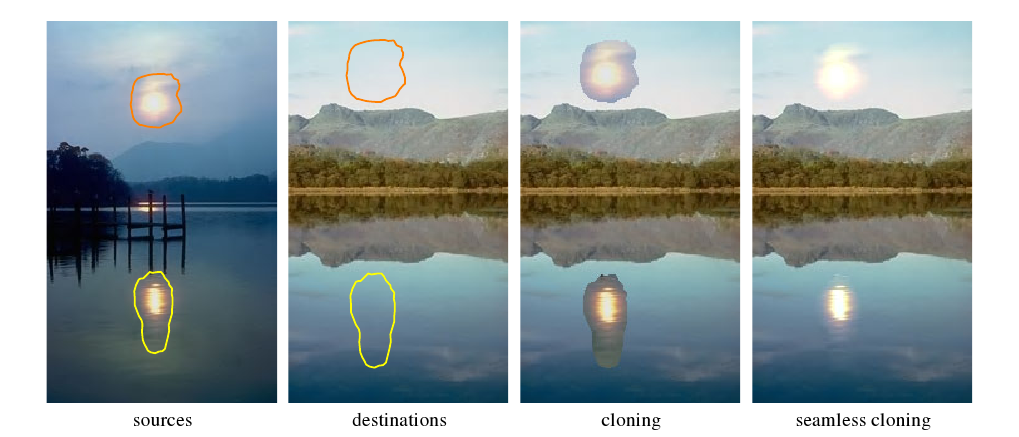
\includegraphics[scale=0.55]{images/cloning.png}
\par\end{centering}

\caption{The seamless blending of regions into a target image using Poisson
  image editing.}
\label{fg:poisson}

\end{figure}

\paragraph{Expression transfer algorithm.}Having established how faces will be reanimated using textures, we can now
summarize the expression transfer algorithm:
\begin{itemize}
\item \textbf{Step 1.} Apply the fitting algorithm to the \textbf{source} video sequence
  to obtain the identity, expression model parameters and the 3D pose parameters
  for every frame.
\item \textbf{Step 2.} Apply the fitting algorithm to the \textbf{target} video sequence
  to obtain the identity, expression model parameters and the 3D pose
  parameters for every frame.
\item \textbf{Step 3.} Compute a sequence of 3D faces using the identity
  parameters along with the 3D pose from the target and the expression parameter
  from the source. Each face in the sequence will share the identity parameter
  but will have different values for the expression and 3D pose
  parameters. These are the faces with transferred expressions.
\item \textbf{Step 4.} For each frame.
\begin{itemize}
\item[\textbullet] Use the geometry and topology of the \textbf{source face} obtained in step 1 to
  find the mouth and the eyebrows.
\item[\textbullet] Use the geometry and topology of the \textbf{target face} obtained in step 2 to
  find the mouth and the eyebrows.
\item[\textbullet] Poisson clone the mouth and the eyebrows from the source texture into
  the target texture using the size of the target mouth and eyebrows as the
  region size.
\end{itemize}
\end{itemize}

\section{System Architecture}
The system architecture of the expression transfer application follows a
model-view-controller (MVC) design. There are three conceptual layers -- the
view layer which is responsible for interacting with the user, the controller
layer which processes the commands coming from the view and the model or data
layer. The MVC architecture is depicted in figure \ref{fg:mvc} 

\begin{figure}[H]
\begin{centering}
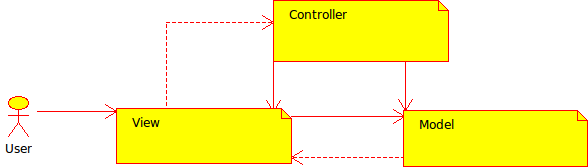
\includegraphics[scale=0.75]{images/mvc.png}
\par\end{centering}

\caption{System architecture of the expression transfer application.}
\label{fg:mvc}
\end{figure}

Each layer contains a number of classes and interfaces, chosen so that the coupling
between layers is decreased and the cohesion inside the layer is increased. 

\subsection{View Layer}
The view layer of the expression transfer application contains the classes which
are responsible for user interface related tasks such as displaying the 3D model
and providing interactive images for feature point selection. There are four
crucial components in the expression transfer view layer. The
OpenGL widget class, a class hierarchy of interactive images, the main
window and the GUI.

\paragraph{OpenGL widget}
The expression transfer application needs to allow the user to view the
estimated 3D model or to view the 3D face scans from the database. The GUI is build with Qt
which supports OpenGL and provides the widget class \texttt{QGLWidget}. This
widget class integrates with the OpenGL graphics interface and includes a canvas
onto which objects can be rendered. The class implements three functions with
protected visibility which
can be overwritten in any class inheriting from \texttt{QGLWidget}. These
functions are \texttt{initializeGL()}, \texttt{resizeGL()} and
\texttt{paintGL()}. The first of these functions, \texttt{initializeGL()}, is
called when the widget class is constructed to set up the rendering context. The function \texttt{resizeGL()} is
called when the window which holds the widget is resized and should be
overwritten so that it correctly sets the viewport and the projection parameters. The most important of
the three function is \texttt{paintGL()} which controls the drawing of the
scene.

In addition to the rendering functions, there are also useful public functions
such as \texttt{bindTexture(.)} and \texttt{grabFrameBuffer(.)} to support
adding texture or grabbing the frame buffer and returning it in form of an
image.

The expression transfer application's view layer includes the class
\texttt{FaceWidget} which extends the \texttt{QGLWidget}. The \texttt{FaceWidget} class overwrites the rendering functions of \texttt{QGLWidget} to allow for a
3D face scan to be displayed. The class also intercepts mouse events so that the
object on the canvas can be rotated or enlarged.

Inheriting from \texttt{FaceWidget}, the class \texttt{CustomizableFaceWidget}
makes it possible to load a custom projection matrix into OpenGL.

\paragraph{Interactive Image Hierarchy}
In a Qt based user interface, images are displayed using the \texttt{QLabel} class. Since the
face transfer application needs to allow the user to select points on the image
it is necessary to extend this base class. The main subclass which stores and
displays clicked points is \texttt{ClickableQLabel}. This class is extended by
\texttt{FeaturePointQLabel} which maps clicked points to corresponding 3D
feature points and \texttt{VectorFieldQLabel} which is used to display an
optical flow vector field.

\paragraph{Main Window}
The GUI is itself is encapsulated in a main window. In the expression transfer application the
main window's functionality is implemented in the class
\texttt{ExpTranWindow}. This class is responsible for all the GUI objects such
as labels, OpenGL widgets and buttons. It also holds references to the controller
layer and connects the signals emitted by the GUI objects to the appropriate
controller objects.
\paragraph{GUI}
The graphical user interface is separated into three tabs. The face tab allows
the user to view a 3D face model and change its expression and identity using
sliders. The design for this tab is shown in figure \ref{fg:facetab}

\begin{figure}[h]
\begin{centering}
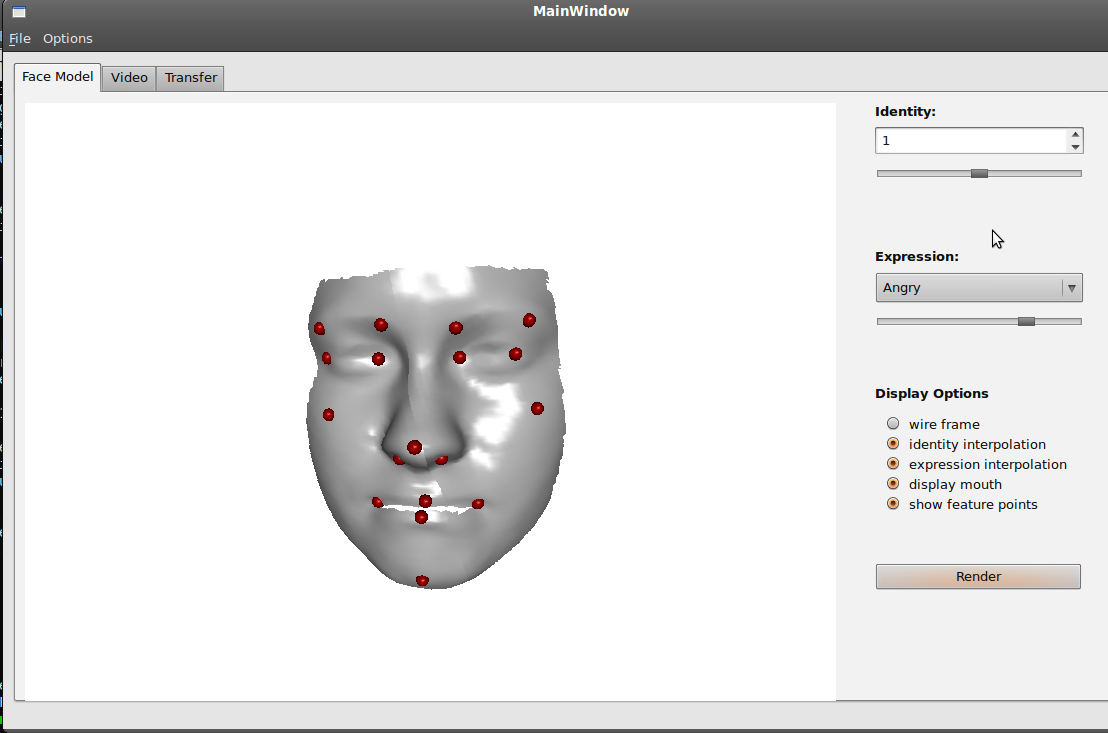
\includegraphics[scale=0.35]{images/facetab.png}
\par\end{centering}

\caption{The face tab part of the GUI which allows the user to view and move the
  3D face.}
\label{fg:facetab}
\end{figure}

\begin{figure}[H]
\begin{centering}
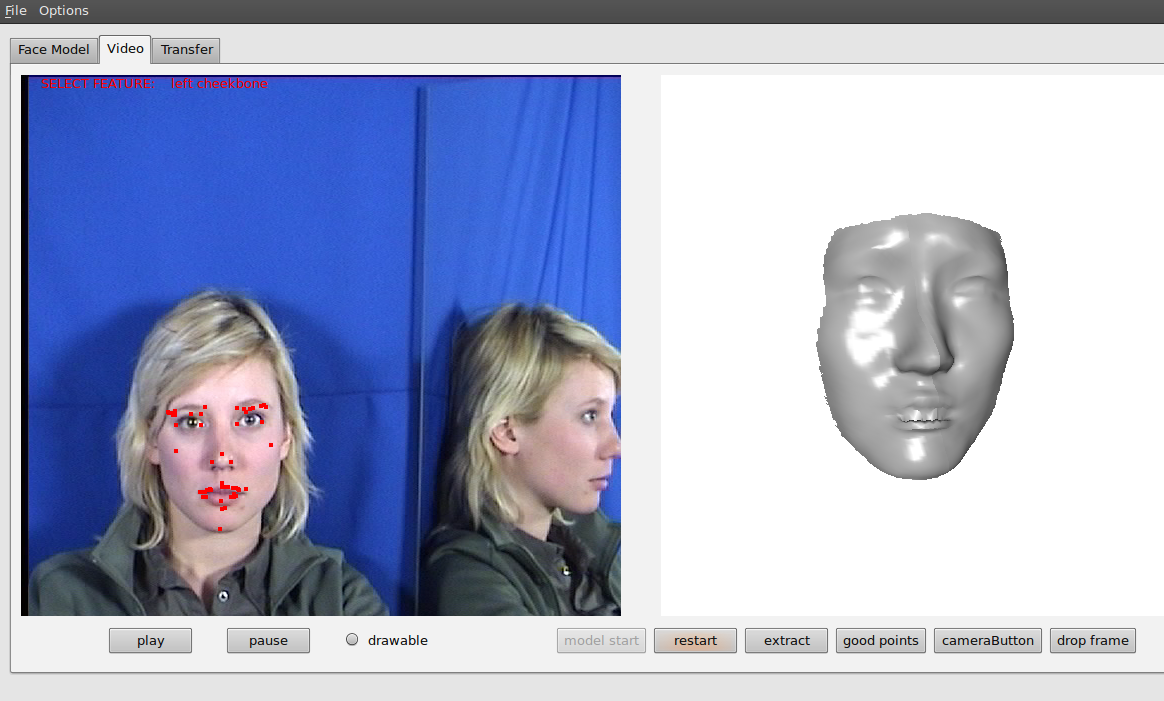
\includegraphics[scale=0.35]{images/videotab.png}
\par\end{centering}

\caption{The video tab which provides model fitting and feature point tracking functionality.}
\label{fg:videotab}
\end{figure}

The face tab also includes an options group which allows the user to customize how
the face is displayed. The menu bar of the window contains a File and an
Options drop down menu. Using the file menu the user can load a .VTK file
containing a face object or a video file to use in the video tab.

The video tab processes the loaded video, providing functionality related to tracking points, extracting 3D
pose and fitting the model to the video. The design of this tab is shown in
figure \ref{fg:videotab} 


This tab contains a \texttt{ClickableQLabel} which represents the current frame
of the video. Feature points can be selected on this frame. The 
OpenGL widget is then used to display the model which is extracted from the image.

The expression transfer functionality is provided in the transfer tab. This tab allows the user to load a
source and a target video files needed for the expression transfer.

\subsection{Model Layer}
The model layer contains classes that participate in constructing and fitting
the tensor based model. A diagram of the class hierarchy in this layer is
depicted in figure \ref{fg:modellayer}


\begin{figure}[H]
\begin{centering}
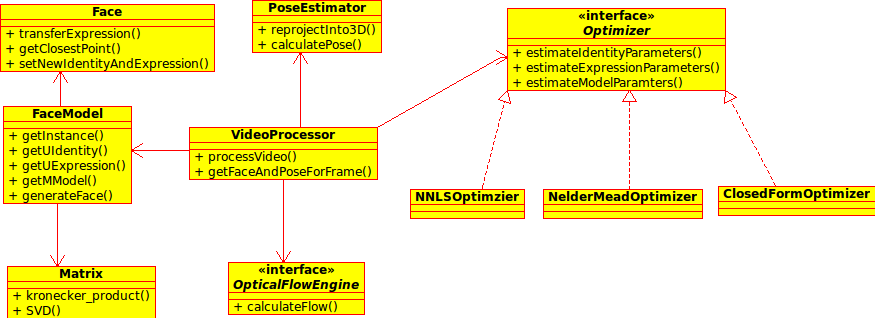
\includegraphics[scale=0.67]{images/modellayer.png}
\par\end{centering}

\caption{UML class diagram of the model layer.}
\label{fg:modellayer}
\end{figure}

The model layer can be divided based on responsibility into two parts. The first
part is composed of the classes which are used to construct the tensor
model and generate new faces. The second part of the model layer is responsible for fitting the model
to an image.

\paragraph{Model Construction}
The model construction algorithm is encapsulated in the persistable \texttt{FaceModel}
class. Persistence means that the tensor model needs to be computed only once. After
the initial computation the class persists the identity mode
matrix, the expression mode matrix and the flattened multilinear model matrix in
a file. When the application is started it will look for this file and if found
it will load these matrices without having to recompute them. 

The \texttt{FaceModel} class follows the singleton design pattern and stores a static instance of a
\texttt{FaceModel} object. It also provides a function to obtain a reference to
this static instance. By hiding its constructor, the class ensures that the only instance of the
class at runtime will be the one static instance. The use of the singleton
pattern makes the code more effective since the mode and model matrices are
quite large and it would require a considerable amount of memory to have more than just one
instance of the \texttt{FaceModel} class at any time.

The tensor model also provides a function to generate new faces given an identity
and expression parameter vector. 

The faces themselves are made up of a number of vertices and the identity and
expression parameters. The application represents a face object using the
\texttt{Face} class.
\paragraph{Model Fitting}
The model fitting algorithm discussed in paragraph \ref{s:fit} is implemented in
the class \texttt{VideoProcessor}. To prevent blocking of the application during the
computation of the fitting algorithm, the class extends \texttt{QThread} so that
each processing of a video can be started in a separate thread.

A \texttt{VideoProcessor} object communicates with an \texttt{Optimizer} object,
a \texttt{PoseEstimator} object and a \texttt{OpticalFlowEngine} object. The
\texttt{Optimizer} provides an interface for model parameter estimation. This
interface is implemented in a number of subclasses each of which applies a
different optimization method to find the parameters. The \texttt{PoseEstimator}
class reprojects points into 3D and calculates the 3D pose using the OpenCV
implementation of the POSIT algorithm. The \texttt{OpticalFlowEngine} is an
interface to a feature tracker algorithm. By default, the engine uses the OpenCV
Kanade-Lucas feature tracker.

The communication between the classes during an invocation of the
\texttt{VideoProcessor} thread is shown in figure \ref{fg:videoproc}

\begin{figure}[H]
\begin{centering}
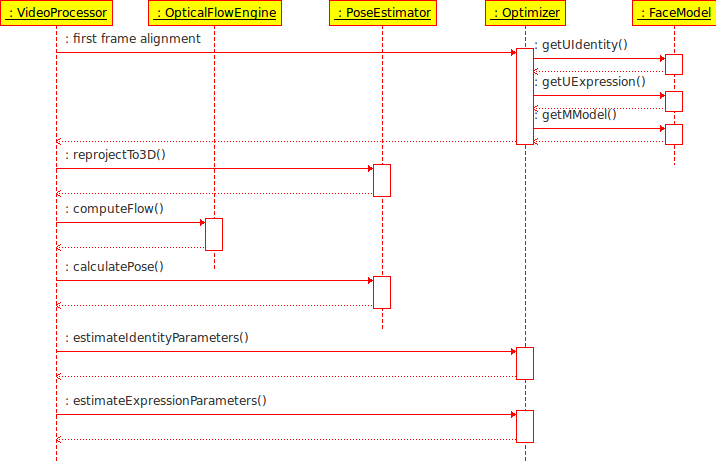
\includegraphics[scale=0.71]{images/videoproc.png}
\par\end{centering}

\caption{The sequence diagram showing an invocation of the
  \texttt{VideoProcessor} thread.}
\label{fg:videoproc}
\end{figure}

\subsection{Controller Layer}
The classes in the controller layer intercept signals and events from the GUI,
process these requests and return the result to the view layer. There are three
controller classes -- one for each tab in the user interface. The
\texttt{FaceTabController} reacts to movements of the sliders by calling the
face generation functions from \texttt{FaceModel} and then updating the OpenGL
widget. The \texttt{VideoTabController} starts \texttt{VideoProcessor} threads
or computes the optical flow using the appropriate classes from the model
layer. Finally, the \texttt{TransferTabController} provides functionality to
transfer expression between two video files. It allows the user to load a source
and a target video file and to start the expression transfer process which
estimates the face model parameters, exchanges the expression and transfers
texture.


\chapter{Results and Evaluation}
The expression transfer application's performance depends heavily on the speed
and accuracy of the fitting algorithm and the expressive power of the tensor
model. This chapter presents results obtained from the application which can be
analyzed to evaluate the performance of the tensor model and the fitting
algorithm designed in chapter 4.
\section{Face Generation}
The model's power depends on its ability to generate a large variety of
different faces. Since the tensor model generates novel faces from linear
combinations of faces from the database its expressive power is limited by the
shape variance inherent in the database. In the face tab of the GUI the user is
allowed to explore this generative power of the model by altering the model
parameters using GUI sliders. The original faces from the database can be
recovered from the model by setting exactly one identity and one expression
slider to one and the rest to zero. 
\begin{figure}[H]
\begin{centering}
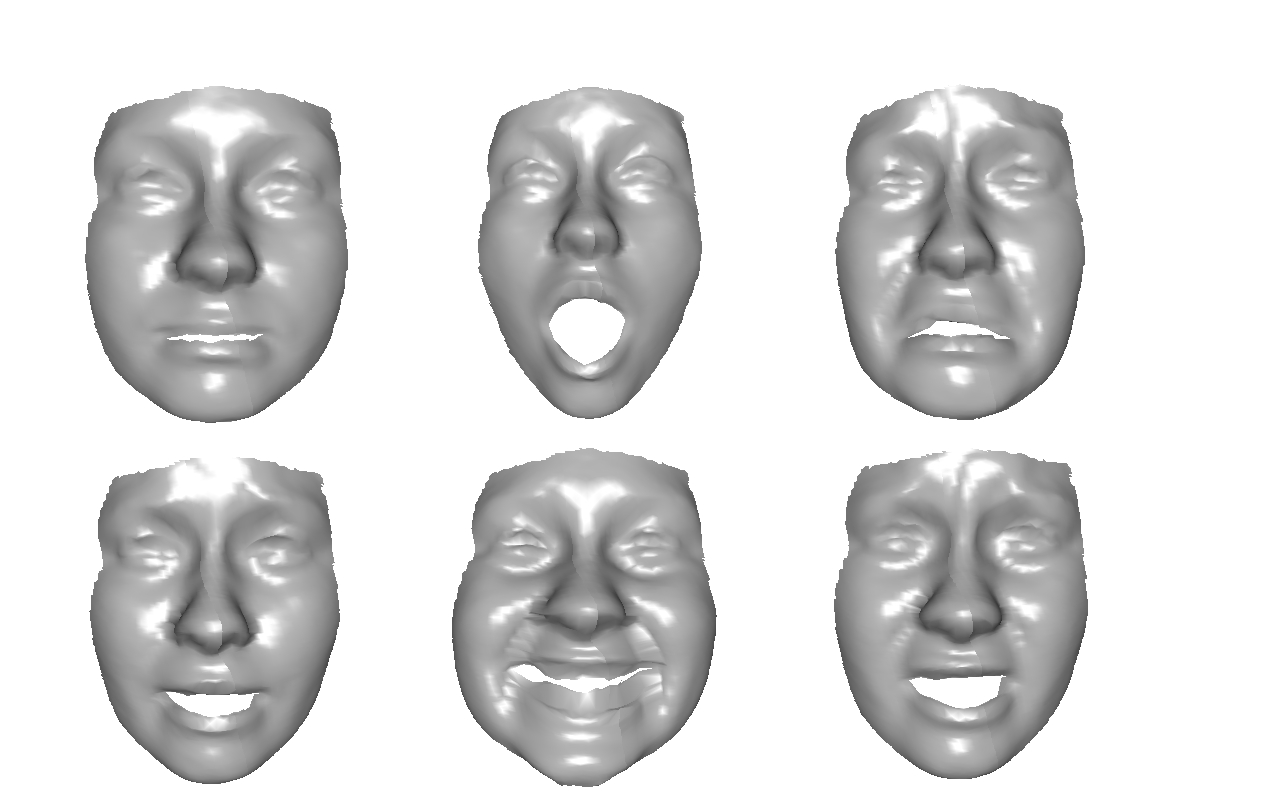
\includegraphics[scale=0.25]{images/faces_generated.png}
\par\end{centering}

\caption{The graphic shows six expressions of the seven
  expressions present in the database. From left to
  right, top to bottom: neutral, surprise, sadness, fear, happiness and disgust.}
\label{fg:facegen}
\end{figure}
 
The expression transfer can use the multilinear model to generate novel faces as
linear combinations of original faces. The variance of the model is thus
equivalent to the variance of the vertices of which the original faces consist. The extent of the variance of a tensor model constructed from the Binghamton database is depicted in figure \ref{fg:faceaddsub}.

\begin{figure}[H]
\centering
\subfloat[Moving a happy face in the negative neutral direction from right to left.]{\label{sfg:happyneg}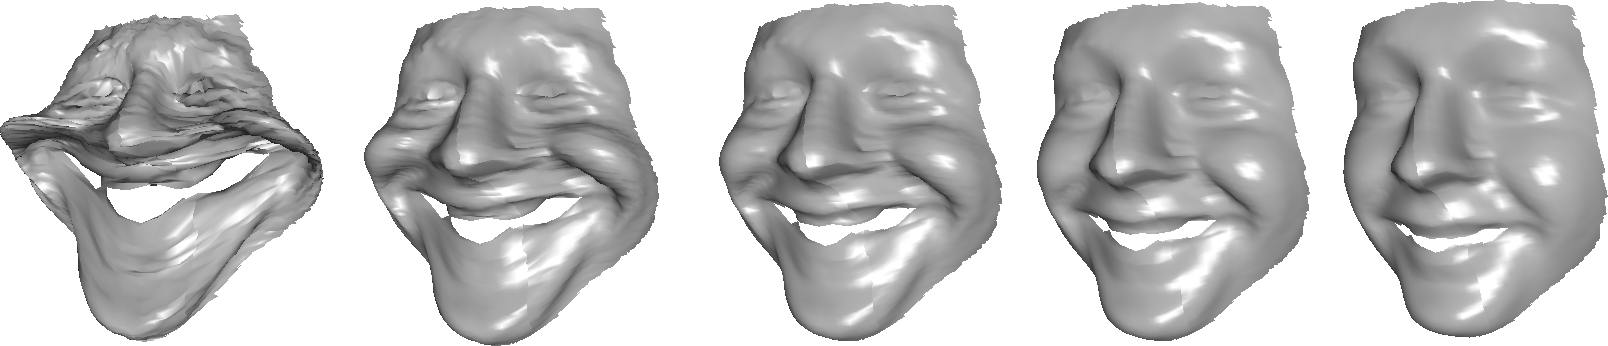
\includegraphics[scale=0.25]{images/sub_neu_from_happy.png}}\\
\subfloat[Moving a neutral face in the negative happy direction from right to left.]{\label{sfg:neghappy}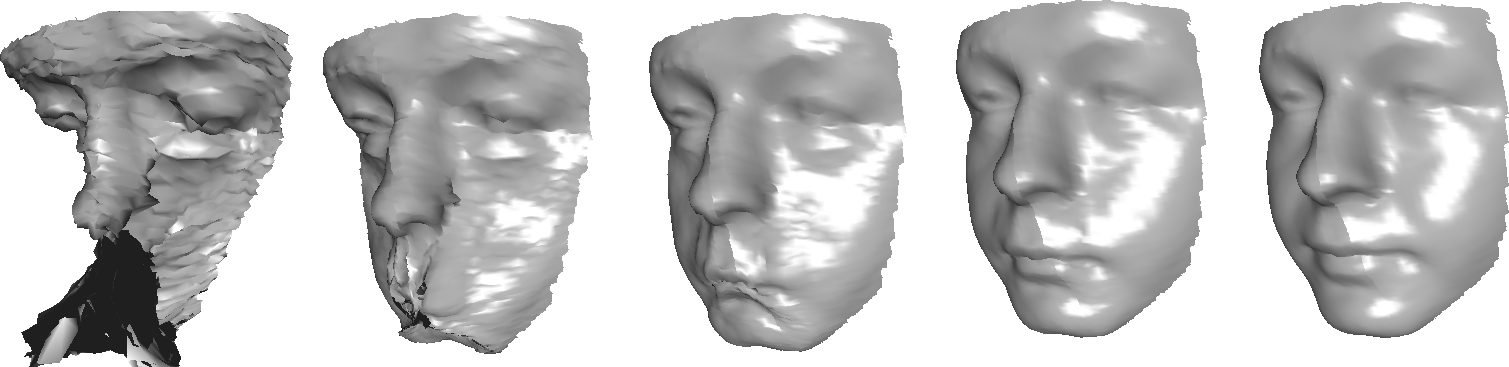
\includegraphics[scale=0.25]{images/sub_happy_from_neutral.png}}

\caption{New expressions are generated by moving the points in the direction of one of
  the vectors of the expression mode matrices. This movement is mathematically
  equivalent to taking a linear combination.}\label{fg:faceaddsub}
\end{figure}

From the results shown in figure \ref{fg:faceaddsub} we can see that by
subtracting too much of one expression from another it is possible to generate
shapes which do not resemble faces. On the other hand, interpolating between
faces always generates realistic faces since no coefficient in the linear
combination can be negative. This means that faces are only added together and
not subtracted from each other. Figure \ref{fg:faceinter} shows experimental
results for interpolating between the base 7 expressions (happy, neutral, angry,
fear, sad, surprise, disgust).

\begin{figure}[H]
\centering
\subfloat[Interpolating between a neutral and surprised
  expression.]{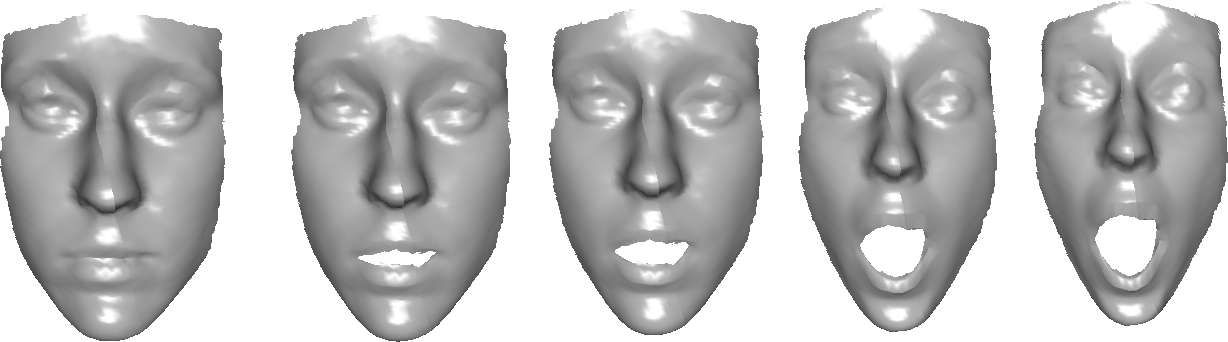
\includegraphics[scale=0.35]{images/interpol_neu_sur.png}}\\

\caption{Generating new face through linear interpolation of the original faces.}\label{fg:faceinter}
\end{figure}

The tensor model is well-suited for expression transfer applications since it to
manipulates the identity and the expression of the subject separately. This
is shown in figure \ref{fg:faceidinter}, where we interpolate the identity
between two subjects from the database first with a neutral expression
and then with a happy expression.

\begin{figure}[H]
\centering
\subfloat[Interpolating between two identities with a neutral expression.]{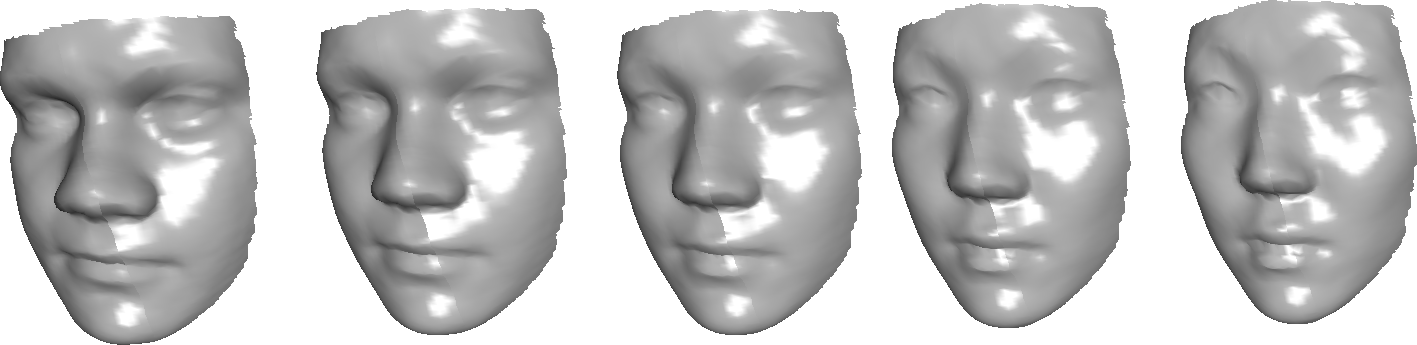
\includegraphics[scale=0.23]{images/ident_interpol.png}}\\
\subfloat[Interpolating between two identities with a happy expression.]{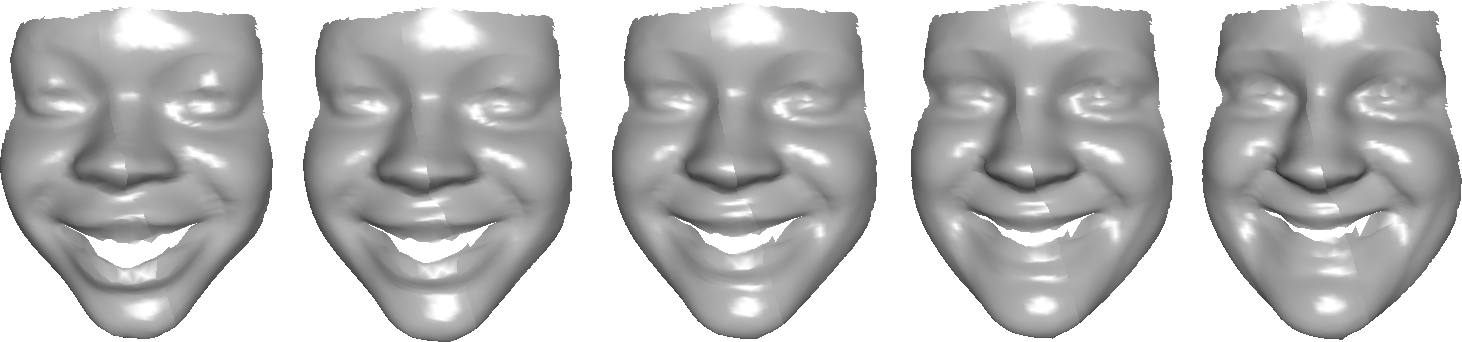
\includegraphics[scale=0.23]{images/id_inerpol_happy.png}}

\caption{Linear interpolation between subjects from the Binghamton database.}\label{fg:faceidinter}
\end{figure}

The fitting algorithm finds the model parameters by minimizing the difference
between projected model feature points and corresponding feature points in the
image. For this approach to work the feature points on the model must move as
they would on a real face. For the pre-processed Binghamton database this holds as can be
seen in figure \ref{fg:featureinter}.

\begin{figure}[H]
\centering
\subfloat[Movement of feature points when interpolating between a neutral and
  fearful expression.]{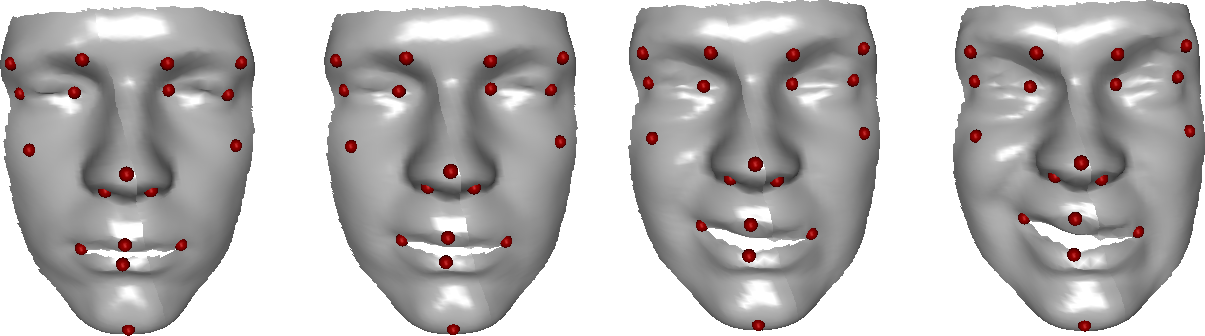
\includegraphics[scale=0.23]{images/fear.png}}\\
\subfloat[Movement of feature points when interpolating between a surprised and
  happy expression.]{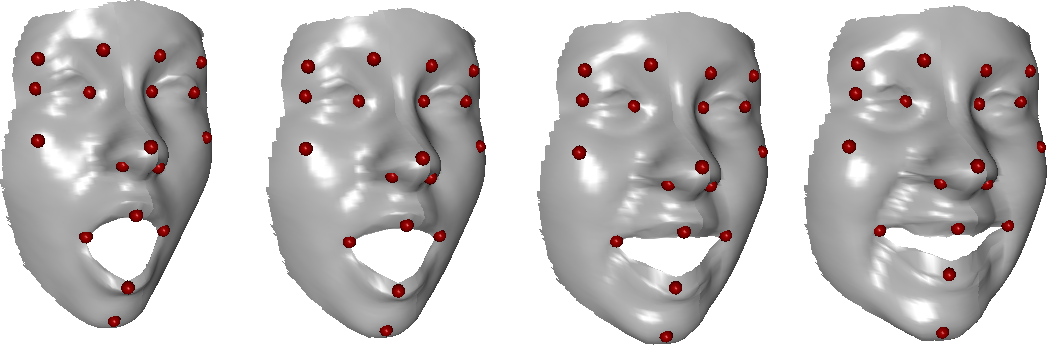
\includegraphics[scale=0.23]{images/happy_surprise.png}}

\caption{The movement of feature points (designated by red spheres).}\label{fg:featureinter}
\end{figure}



\section{Tracking Results}
The most important part of the fitting algorithm is feature point
tracking. Without identifying how the feature points are moving in the image, it
is impossible to determine the correct expression and 3D pose during using the
fitting algorithm. The task of tracking points becomes more difficult if there
are changes in lighting in the image or if the object is moving very
quickly. Likewise, points located in large areas of constant texture often drift
away from their true positions. 

The main parameter which affects the performance of the Kanade-Lucas feature
point tracker is the window size. As discussed in section \ref{s:kanade}, the
window size is the area around the point, the texture of which the tracker uses
to determine the movement of the point. If the window size is chosen too small
then points may jump around since the texture in the window is too small to be
unique enough. Figure \ref{fg:3opt} shows the tracking of a moving face with
a $3 \times 3$ window size around every feature point.

\begin{figure}[H]
\begin{centering}
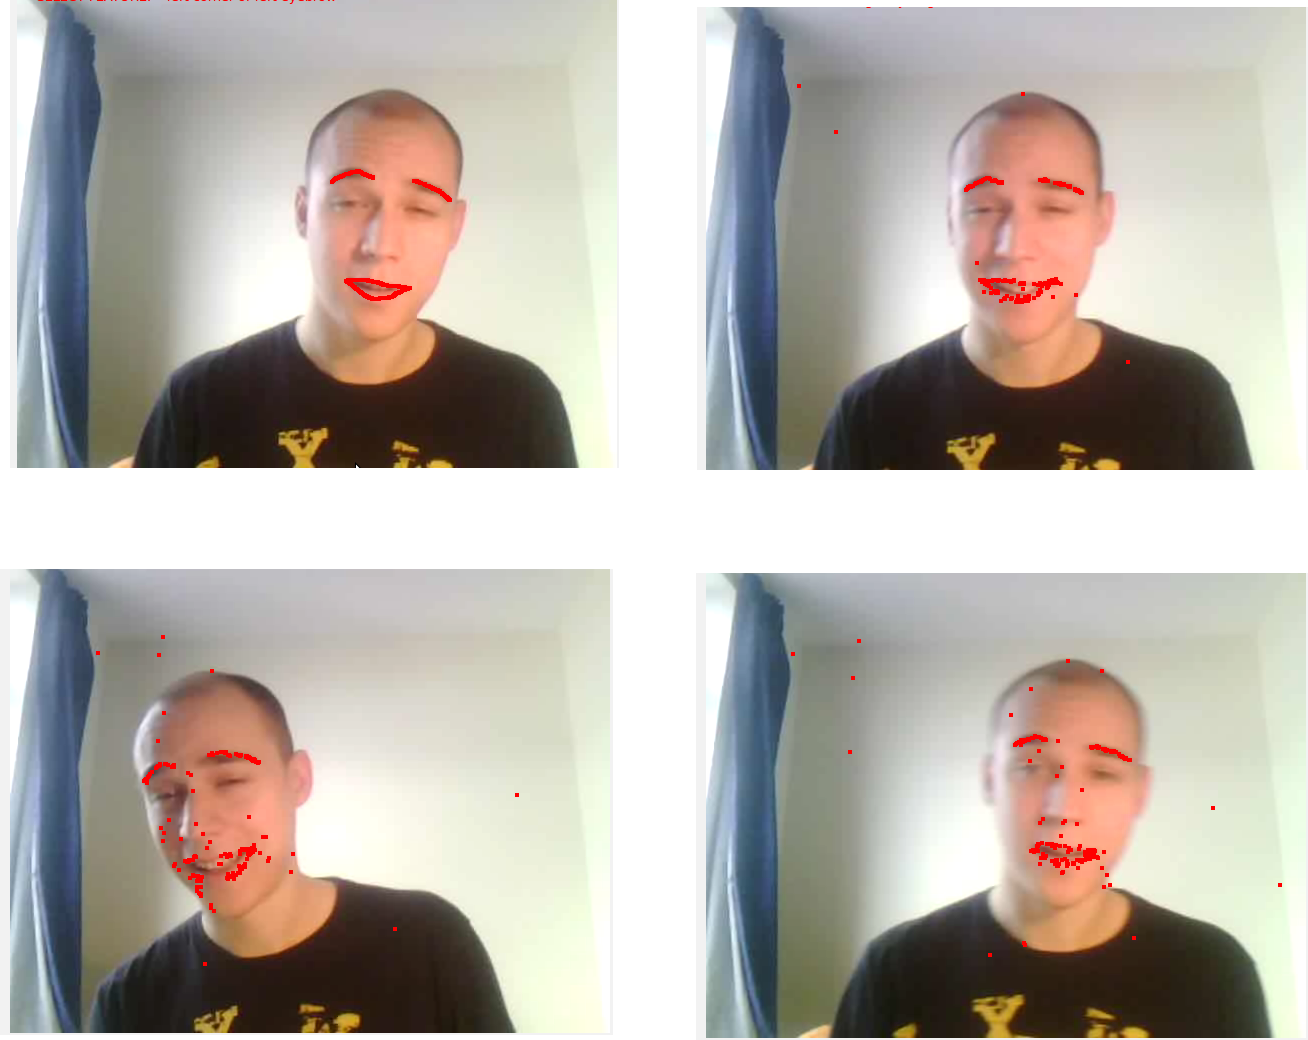
\includegraphics[scale=0.28]{images/3x3opt2.png}
\par\end{centering}

\caption{Tracking of feature point using a $3 \times 3$ window size. A large
  number of feature points jump into incorrect positions, since the
  window size is too small.}
\label{fg:3opt}
\end{figure}


If, on the other hand, the window size is chosen too large then small movements of
points will be subdued. This happens because even though textures close to the
point change, the ones far from the point may not and the evidence from the far
off textures will outweigh the small contribution from the nearby
textures. Figure \ref{fg:50opt} shows tracking with a $50 \times 50$ window
size. It can be seen that although points are not jumping anymore, the smile and
the eyebrows do not move as much as the actual pixels of the image.

\begin{figure}[H]
\begin{centering}
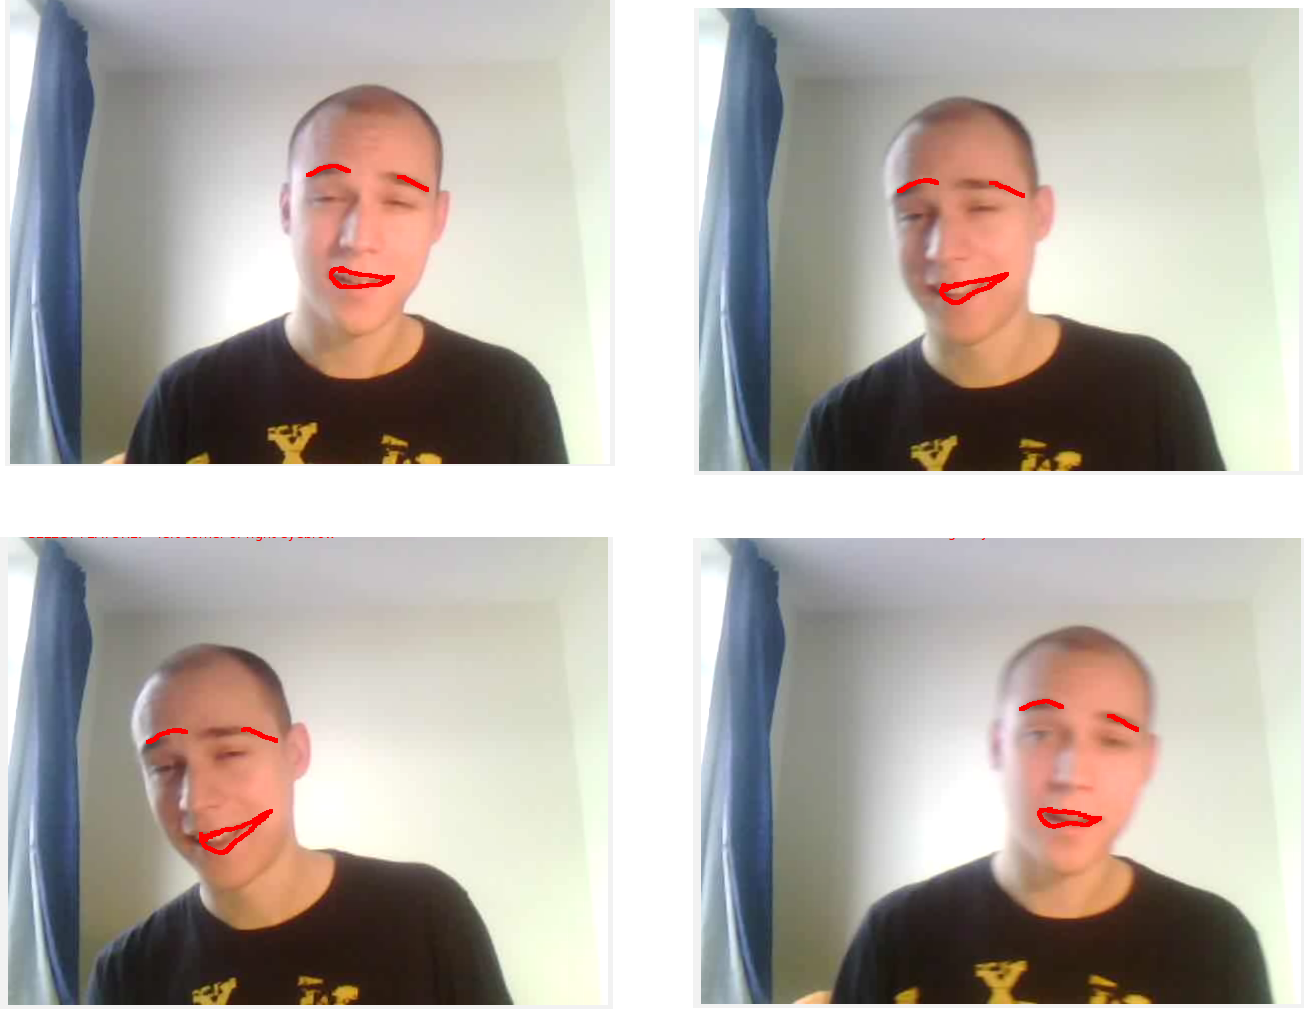
\includegraphics[scale=0.27]{images/50x50opt.png}
\par\end{centering}

\caption{Tracking of feature point using a $50 \times 50$ window size. The
  features do not follow their true counterparts because the window size is too large.}
\label{fg:50opt}
\end{figure}

\begin{figure}[H]
\begin{centering}
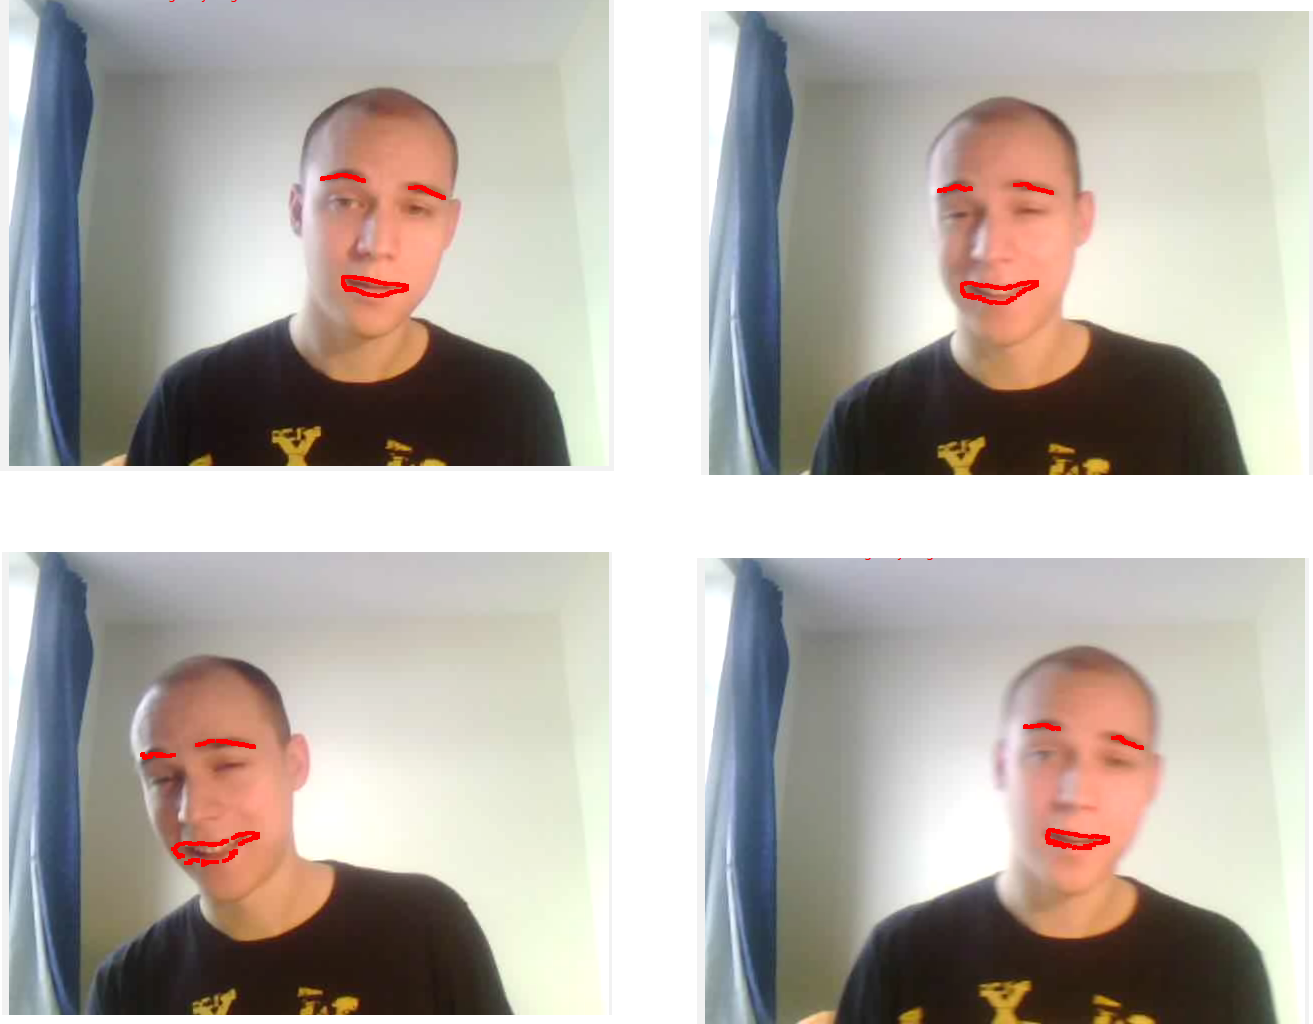
\includegraphics[scale=0.27]{images/8x8opt.png}
\par\end{centering}

\caption{Best tracking results obtained using a $15 \times 15$ window size.}
\label{fg:8opt}
\end{figure}
\section{Optimization Results}
The quality of the model and 3D pose parameter estimation depends on the
selection of the feature points. This is due to the face that the first frame
alignment is calculated purely using the user provided (or automatically
located) feature points. The first frame alignment is then used to determine the
3D model correspondences of a
large number of newly generated feature points. These correspondences bias the
fitting process toward the identity, expression and 3D pose of the first
alignment, especially when the performance in the video is not very dynamic. So
if the first frame alignment is
very different from the true identity, expression and 3D pose of the subject
then the fitting algorithm also returns an incorrect estimate of the face.

On the other hand, the user cannot be expected to input a large number of
feature points and an automatic algorithm is likewise only effective for a small
number of unique features such as the mouth corners, eye corners etc.
\section{Expression Transfer Results}

\section{Performance}
The expression transfer application was tested on the following system
\begin{itemize}
\item \textbf{System Type:} Thinkpad Laptop
\item \textbf{Operating System:} Ubuntu 9.10 (kernel 2.6.31-22)
\item \textbf{Processor:} Intel(R) Core(TM)2 Duo CPU P8400 @ 2.26GHz
\item \textbf{RAM:} 2GB DDR2
\item \textbf{Graphics Card:} Intel GMA 4500MHD
\end{itemize}
On this system, constructing a tensor model from the Binghamton databases with
5090 vertices, 7 expressions and 56 identities averages at around 2 minutes. This
includes loading the data from the database and computing the HOSVD.

Fitting the algorithm to using a linear combination algorithm with
regularization takes less than about a third of a second per frame. 

Fitting the model parameters by enforcing linear interpolation through
non-negativity constraints and solving using the sequential coordinate-wise
non-negativity least squares algorithm averages at around 25 seconds for 40
frames and around 28 seconds for 50 frames for 100 feature points, thus averaging at a little over 0.6
seconds per frame. 

\chapter{Conclusion}
To summarize, we developed the expression transfer application for 
\section{Future Work}
As part of the expression transfer application, we constructed a deformable model from a simple database of 3D face scans displaying
expressions. An intriguing prospect for future work would be to perform data
gathering and construct larger, more powerful 3D databases,
with more attributes than identity and expression. For example it would be
interesting to build an appearence tensor model with attributes for expressions,
identities, lighting and texture of the faces as well. Tensor based shape models of other objects
such as hands and entire bodies are an area which has not been researched as
thoroughly as face models by the computer vision community. It would therefore
be possible to contribute to the deformable modelling field by exploring tensor models
of such objects. Constructing and fitting the model using a new database would not necessitate the reworking of the algorithms derived in the
paper. The HOSVD and the fitting algorithm could be easily adapted to work with
databases not consisting of face scans by simply adapting the number of
parameters and mode matrices. 

Of course, to build a new database it would be necessary to perform 3D data
gathering. It should however be possible to perform this gathering without the
need for expensive equipement. Structured light based scanning equipment and other 3D shape recovery approaches
such as computational or photometric stereo are increasingly becoming more readily
available to casual users and they would lend themselves well for data gathering
purposes. The application could for instance be extended to allow the user to
perform their own data gathering on an object of their choosing and then to
construct a tensor model from it. If it were not possible to gather 3D despite the availability of data gathering techniques,
more variablity could be introduced to existing databases by utilizing a FEM based
model to generate new faces and using these to expand the database.

To improve the usability of the application it would also be intriguing to link
an feature point detection algorithm into the expression transfer algorithm. An
automatic feature detection framework such as the Viola-Jones feature tracker
\cite{viola} would make the application more accessible to casual users. The automatic detector could be trained to locate corners of the
mouth, eyebrows or the tip of the nose. These points are easily distinguishable
and are conveniently already utilized as feature points in the application. Even an external feature point tracker could therefore be
seamlessly linked with the application if it produced a set of 2D feature
point coordinates which would then be used by the expression transfer fitting algorithm.

The main limitation we encountered with the shape tensor-based model is the need for
correspondences between feature and model points. Correspondences are not
elegant and weaken the power of the model fitting approaches. This limitation
could be overcome by utilizing an appearence based tensor model. Since this
model generates a textured representation of the face its projection into
2D is a textured image of the face. It therefore is less constrained in how the
error is computed meaning that more elegant and flexible fitting algorithms
could be developed. To construct such a model it would be necessary to known the
RGB values at every vertex so a database with texture maps and texture
coordinates would be required. An tensor-based model of appearence would also
be able to reanimate faces without having to resort to Poisson image editing
techniques.

Lastly, a future project could explore the performance of Newton and quasi-Newton fitting
algorithms for the tensor model of shape. Section \ref{s:minerror} provides the starting point of such
approahces and the derives two of the four optimal parameters non-linear equations.
\bibliographystyle{plain}
\bibliography{references}

\end{document}
